\documentclass{article}
%build with recipe latexmk
\usepackage[utf8]{inputenc}
\usepackage[T1]{fontenc}
\usepackage{textcomp}

\usepackage{fancyhdr}
\pagestyle{fancy}

\usepackage{tcolorbox}
\usepackage{ stmaryrd }
\tcbuselibrary{theorems}
\usepackage{babel}
\usepackage{enumerate}
\usepackage{amsmath, amssymb, amsthm}
%\usepackage{a4wide}
\usepackage{float}
\usepackage{pgfplots}
\usepgfplotslibrary{fillbetween}
\usepackage{tikz-cd}
\usepackage{tikz}
\usepackage{graphicx}
\usepackage{caption}
\usepackage{wrapfig}
\usepackage{setspace}
\setstretch{1.1}
\usepackage{color}
\usepackage{hyperref}
\hypersetup{
    colorlinks=true, %set true if you want colored links
    linktoc=all,     %set to all if you want both sections and subsections linked
    linkcolor=black,  %choose some color if you want links to stand out
}
\usepackage{stackrel}

\theoremstyle{definition}
\newtheorem{theorem}{Theorem}[section]
\newtheorem{lemma}[theorem]{Lemma}
\newtheorem{cor}[theorem]{Corollary}
\newtheorem{prop}[theorem]{Proposition}
\newtheorem{example}{Example}[section]
\newtheorem{defn}{Definition}[section]
\newtheorem*{claim*}{Claim}

\title{Part III - Modular Forms
    \\ \large
    Lectured by Jack Thorne
}
 
\author{Artur Avameri}
\date{Michaelmas 2023}
 
\setcounter{section}{0}
 
\begin{document}
\maketitle
\tableofcontents
\newpage

\section{Introduction}

\marginpar{06 Oct 2022, Lecture 1}

\begin{defn}
    We define the following groups:
    \begin{align*}
        &\mathfrak{h} = \{\tau \in \mathbb{C} \mid \text{Im}(\tau)>0\}\\
        &GL_2(\mathbb{R})^{+} = \{g \in GL_2(\mathbb{R}) \mid \det(g)>0\}\\
        &\Gamma(1) = SL_2(\mathbb{Z}) = \{g \in M_2(\mathbb{Z}) \mid  \det(g)=1\} .
    \end{align*}
    Note that $\Gamma(1)$ is a subgroup of $GL_2(\mathbb{R})^+$.
\end{defn}
\begin{lemma}
    $GL_2(\mathbb{R})^+$ acts transitively on $\mathfrak{h}$ by Möbius transformations.
\end{lemma}
\begin{proof}
    Let $g = \begin{pmatrix} a & b\\c&d \end{pmatrix} \in GL_2(\mathbb{R})^+, \tau \in \mathfrak{h}$. Then \[
    \text{Im}(g \tau) = \frac{1}{2i}\left(\frac{a \tau + b}{c \tau + d} - \frac{a \overline{\tau}+ b}{c \overline{\tau } + d} \right) = \frac{1}{2i} \frac{(ad-bc)(\tau - \overline{\tau})}{|c \tau + d|^2} = \frac{\det(g) \text{Im}(\tau)}{|c \tau + d |^2} > 0,
    \]
    so $g \tau \in \mathfrak{h}$. This action is transitive since \[
    x + iy  \in \mathfrak{h} \implies \begin{pmatrix} y & x \\ 0 & 1 \end{pmatrix} i  = x + iy,
    \]
    so everything in $\mathfrak{h}$ is conjugate to $i$.   
\end{proof}
\begin{defn}
    If $g = \begin{pmatrix} a & b\\ c & d\end{pmatrix}\in GL_2(\mathbb{R})^+$ and $\tau \in \mathfrak{h}$, then define \[
    j(g, \tau) =  c \tau + d.
    \]
    This is called a \textbf{modular cocycle}.
    If $k \in \mathbb{Z}$ and $f : \mathfrak{h} \to \mathbb{C}$, then \[
    f |_k[g]: \mathfrak{h} \to \mathbb{C}
    \]
    is defined by \[
    f |_k[g](\tau) = \det(g)^{k-1} f(g \tau) j(g, \tau)^{-k}.
    \]
    This is the \textbf{weight $k$ action of $g$ on $f$}.
\end{defn}
\begin{lemma}
    This is a right action of $GL_2(\mathbb{R})^+$: if $g,h \in GL_2(\mathbb{R})^+$, then $$f|_k[gh] = (f|_k[g])|_k[h].$$
\end{lemma}
\begin{proof}
    We compute
    \begin{align*}
        &(f|_k[g])|_k[h](\tau) = \det(h)^{k-1}f|_k[g](h \tau) j(h, \tau)^{-k} = \\
        &\det(h)^{k-1}\det(g)^{k-1}f(g h \tau) j(g, h \tau)^{-k} j(h, \tau)^{-k}  \stackrel{?}{=}\\
        & \det(gh)^{k-1} f(gh \tau) j(gh, \tau)^{-k} = f|_k[gh](\tau). 
    \end{align*}
    Hence we need to check that $j(gh, \tau) = j(gh, \tau)j(h, \tau)$. Note that if $g = \begin{pmatrix} a & b \\ c & d \end{pmatrix}$, then \[
    g \begin{pmatrix} \tau \\ 1 \end{pmatrix} = \begin{pmatrix} a \tau + b\\ c \tau + d \end{pmatrix} = j(g,\tau)\begin{pmatrix} g \tau \\ 1 \end{pmatrix}.
    \]
    We now get\[
    j(gh, \tau) \begin{pmatrix} g h \tau \\ 1 \end{pmatrix} = gh \begin{pmatrix} \tau \\ 1 \end{pmatrix} = g \left( j(h, \tau) \begin{pmatrix} h \tau \\ 1 \end{pmatrix}\right) = j(h, \tau) j(g, h \tau) \begin{pmatrix} g h \tau \\ 1 \end{pmatrix},
    \]
    which finishes the computation and proof.
\end{proof}
\textbf{Formulae.} For $g \in GL_2(\mathbb{R})^+, \tau \in \mathfrak{h}$, we have \begin{align*}
    \text{Im}(g \tau) = \det(g) \frac{\text{Im}(\tau)}{|j(g,\tau)|^2} \text{ and } j(g,\tau) \begin{pmatrix} g \tau \\ 1 \end{pmatrix} = g \begin{pmatrix} \tau \\ 1 \end{pmatrix}.
\end{align*} 
\begin{defn}
    Let $k \in \mathbb{Z}$ and $\Gamma \le \Gamma(1)$ of finite index\footnote{In other words, $\Gamma$ is a (finite index) subgroup of $\Gamma(1)$.}. A \textbf{weakly modular function of weight $k$ and level $\Gamma$} is a meromorphic function $f : \mathfrak{h} \to \mathbb{C}$ which is invariant under the weight $k$ action of $\Gamma$, i.e. such that $$\forall \tau \in \mathfrak{h}, \forall \gamma \in \Gamma, f|_k(\gamma) = f.$$
\end{defn}
We will define modular forms next time: they are weakly modular functions which are holomorphic both in $\mathfrak{h}$ and at $\infty$.
\vspace{1mm}
 
It is a fact that modular forms of fixed weight and level live in finite-dimensional $\mathbb{C}$-vector spaces called $M_k(\Gamma)$. These form the main objects of study in this course.
\vspace{1mm}
 
\textbf{Motivation.} Why study modular forms?
\begin{enumerate}[(1)]
    \item They are related to the theory of elliptic functions.
    Let $E/\mathbb{C}$ be an elliptic curve and $\omega$ a holomorphic non--zero 1--form. Then there exists a unique lattice\footnote{i.e. a discrete cocompact subgroup, or an abelian subgroup which is freely generated by two elements that are linearly independent over $\mathbb{R}$.} $\Lambda \in \mathbb{C}$ and isomorphism $\phi : \mathbb{C}/\Lambda \to E$ such that $\phi^*(\omega) = dz$. Then $E$ is isomorphic to the elliptic curve $y^2 = 4x^3 - 60G_4(\Lambda)x - 140G_6(\Lambda)$ where if $k \in \mathbb{Z}$, then $G_k(\Lambda) = \sum_{\lambda \in \Lambda - \{0\}}^{} \lambda^{-k}$. This converges absolutely for $k>2$.

    If $\tau \in \mathfrak{h}$, then $\Lambda \tau = \mathbb{Z} \tau \oplus \mathbb{Z} \subset \mathbb{C}$ is a lattice and $G_k(\tau) = G_k(\Lambda_\tau)$. This is a modular form of weight $k$ and level $\Gamma(1)$, called an Eisenstein series.
    \vspace{1mm}
     
    $\mathfrak{h}/SL_2(\mathbb{Z})$ can be identified with the set of (isomorphism classes of) elliptic curves over $\mathbb{C}$.
    \item Modular forms $f$ have Fourier expansions $\sum_{n \in \mathbb{Z}}^{} a_n g^n$, $a_n \in \mathbb{C}$ and they often serve as a generating functions for arithmetically interesting sequences $a_n$.
    \vspace{1mm}
     
    For example, take $\theta(\tau) = \sum_{n \in \mathbb{Z}}^{} e^{\pi i n^2 \tau}$. If $k \in 2\mathbb{N}$, then $\theta^{k}$ is a modular form with $q$--expansion $\theta^{k} = \sum_{n \in \mathbb{Z}}^{} r_k(n) e^{\pi i n \tau}$, where $r_k(n)$ is the number of ways of writing $n$ as a sum of $k$ squares, i.e. $r_k(n) = |\{x \in \mathbb{Z}^k \mid \sum_{i=1}^{k} x_i^2 = n\}|$.
    By expressing $\theta^k$ in terms of other modular forms, we can prove formulae such as $r_4(n) = 8 \sum_{d \mid n, 4 \nmid d}^{} d$.
    \item The Riemann zeta function $\zeta(s)$ is an important object of study. Its pleasant features include:
    \begin{itemize}
        \item The Euler product $\zeta(s) = \prod_{p}^{} (1-p^{-s})^{-1}$.
        \item It has a meromorphic continuation to $\mathbb{C}$ and has a functional equation relating $\zeta(s)$ and $\zeta(1-s)$.
    \end{itemize}
    A Dirichlet series $\sum_{n\ge 1}^{} a_n n^{-s}$ which has similar properties (Euler product, meromorphic extension, some nice function equation) is called an $L$--function. Modular forms can be used to construct interesting examples of $L$--functions. In practice, we take $M_k(\Gamma)$ and decompose it under Hecke operators to get Hecke eigenforms, the nicest possible modular forms, which have the above properties.
    \item The Langlands program predicts a relation between modular forms and objects in arithmetic geometry. A special case of this is the modularity conjecture, which says that there is a bijective correspondence between elliptic curves $E/\mathbb{C}$ up to isogeny and the set of Hecke eigenforms of weight 2. This implies Fermat's last theorem. Note that this is formulated in the language of Hecke operators and $L$--functions.
\end{enumerate}
\textbf{Homework.} There is a handout on Moodle called ''Reminder on Complex Analysis''. Have a look at it before the next lecture.

\newpage

\section{Modular Forms on $\Gamma(1)$}

\marginpar{09 Oct 2022, Lecture 2}

\textbf{Reminder.} A \textbf{meromorphic} function in an open subset $U \subset \mathbb{C}$ is a closed subset $A \subset U$ and a holomorphic function $f : U \setminus A \to \mathbb{C}$ such that $\forall a \in A$, $\exists \delta > 0$ such that $D^*(a,\delta) \subset U\setminus A$ and $\exists n \ge 0$ such that $(z-a)^n f(z)$ extends to a holomorphic function in $D(a,\delta)$.
\vspace{1mm}
 
$f$ then has a Laurent expansion $\sum_{m \in \mathbb{Z}}^{} a_m (z-a)^{m}$ valid on $D^*(a,\delta)$.

\begin{lemma}
    Let $f$ be a weakly modular function of weight $k$ and level $\Gamma(1)$. Then there exists a meromorphic function $\tilde{f}$ in $D^*(0,1)$ (the ''$q$-disk'') such that $$f(\tau) = \tilde{f}(e^{2\pi i \tau}).$$
\end{lemma}
\begin{proof}
    $f$ is meromorphic in $\mathfrak{h}$ by assumption. Take $\gamma = \begin{pmatrix} 1 & 1 \\ 0 & 1 \end{pmatrix} \in \Gamma(1)$. Then $f|_h[\gamma](\tau) = f(\gamma \tau) = f(\tau)$, as $f$ is invariant under the weight $k$ action of $\gamma$. But also $f(\gamma \tau) = f(\tau+1)$, so $f$ is periodic. 
    \vspace{1mm}
     
    Now map a strip of $\mathfrak{h}$ of width 1 to $D^*(0,1)$ by $\tau \mapsto e^{2 \pi i \tau}$. Let $a \in D^*(0,1)$ and $\delta>0$ be such that $D(a,\delta) \subset D^*(0,1)$. Define $\tilde{f}$ on $D(a,\delta)$ by $$\tilde{f}(q) = f\left(\frac{1}{2\pi i} \log q\right),$$ for any branch of $\log$ defined in $D(a,\delta)$. This is meromorphic and independent of the choice of the branch of log, as $f$ is periodic with period 1. This defines $\tilde{f}$ in $D^*(0,1)$. Finally, $\tilde{f}$ is unique since $\tau \mapsto e^{2\pi i \tau}$ is surjective.
\end{proof}

If $\tilde{f}$ extends to a meromorphic function\footnote{This might not be the case if the set of poles has a limit inside the disk.} in $D(0,1)$, then $\exists \delta > 0$ such that $\tilde{f}$ has a Laurent expansion $\tilde{f}(q) = \sum_{n \in \mathbb{Z}}^{} a_n q^n$ valid in $D^*(0,\delta)$. 
\vspace{1mm}
 
In the region $\{\tau \in \mathfrak{h} \mid \text{Im}(\tau) > \frac{1}{2\pi} \log \delta\}$, we have $$f(\tau) = \sum_{n \in \mathbb{Z}}^{} a_nq^n,$$ where $q = e^{2\pi i \tau}$. This is called the \textbf{$q$--expansion} of the weakly modular function $f$.

\begin{defn}
    Let $f$ be a weakly modular function of weight $k$ and level $\Gamma(1)$. We say that $f$ is \textbf{meromorphic at $\infty$} if $\tilde{f}$ extends to a meromorphic function in $D(0,1)$. \vspace{1mm}
     
    We say $f$ is \textbf{holomorphic at $\infty$} if $\tilde{f}$ is meromorphic at $\infty$ and has a removable singularity at $q = 0$. In this case, we define $$f(\infty) = \tilde{f}(0) = \lim_{\text{Im}(\tau) \to \infty}f(\tau).$$
    \vspace{1mm}
     
    We say $f$ \textbf{vanishes at $\infty$} if $f$ is holomorphic at $\infty$ and $f(\infty)=0$.
\end{defn}
\begin{defn}
    A \textbf{modular function} (of weight $k$ and level $\Gamma(1)$) is a weakly modular function (of weight $k$ and level $\Gamma(1)$) which is meromorphic at $\infty$.
    \vspace{1mm}
     
    A \textbf{modular form} is a weakly modular function which is holomorphic in $\mathfrak{h}$ and holomorphic at $\infty$.
    \vspace{1mm}
     
    A \textbf{cuspidal modular form} is a modular form that vanishes at $\infty$.
\end{defn}

\textbf{Remark.} We let $M_k(\Gamma(1))$ denote the set of modular forms of weight $k$ and level $\Gamma(1)$. We write $S_k(\Gamma(1))$ for the set of cuspidal modular forms of weight $k$, level $\Gamma(1)$. Note $S_k(\Gamma(1)) \subset M_k(\Gamma(1))$. These are $\mathbb{C}$--vector spaces. If $k$ is odd, then these both only contain the zero function, since taking $\gamma = \begin{pmatrix} -1 & 0 \\ 0 & -1 \end{pmatrix} \in \Gamma(1)$ gives $f|_k[\gamma](\tau) = f(\tau)(-1)^k = f(\tau)$.
\vspace{1mm}
 
We now consider even weights only. If $k \in \mathbb{Z}$ is even, let \[
G_k(\tau) = \sum_{\lambda \in \Lambda_\tau \setminus 0}^{} \lambda^{-k} = \sum_{(m,n) \in \mathbb{Z}^2 \setminus  0}^{} (m \tau + n)^{-k},
\]
where $\Lambda_\tau = \mathbb{Z} \tau \oplus \mathbb{Z}$ for any $\tau \in \mathfrak{h}$. 
\vspace{1mm}
 
If $\gamma \in \Gamma(1)$, then formally we have $$G_k|_k[\gamma](\tau) = G_k(\gamma \tau)j(\gamma, \tau)^{-k} = \sum_{\lambda \in \Lambda_{\gamma \tau} \setminus 0}^{} \lambda^{-k} j(\gamma, \tau)^{-k},$$
but $\Lambda_{\gamma \tau} = \mathbb{Z} \frac{a \tau + b}{c \tau +d} \oplus \mathbb{Z} = (c \tau + d)^{-1}\left(\mathbb{Z}(a \tau + b) \oplus \mathbb{Z}(c \tau + d)\right) = (c \tau + d)^{-1} \Lambda_\tau$. Hence 
\begin{align*}
    G_k|_k[g](\tau) &= \sum_{\lambda \in (c \tau + d)^{-1} \Lambda_\tau \setminus 0}^{} \lambda^{-k} (c \tau +d)^{-k}\\ &= \sum_{\lambda \in \Lambda_\tau \setminus 0} ((c \tau + d)^{-1}\lambda)^{-k}(c \tau + d)^{-k} = G_k(\tau).
\end{align*}

This is justified only when the series defining $G_k(\tau)$ converges absolutely. Hence:
\begin{prop}
    Let $k > 2$ be an even integer. Then $G_k(\tau)$ converges absolutely and defines a modular form of weight $k$ and level $\Gamma(1)$ which has   $G_k(\infty) = 2\zeta(k)$. $G_k$ is the \textbf{weight $k$ Eisenstein series}.
\end{prop}
We will later see that $M_2(\Gamma(1)) = 0$.
\begin{proof}
    We want to show absolute and locally uniform convergence in $\mathfrak{h}$. This will show that $G_k$ is holomorphic by complex analysis. Let $A\ge 2$ and define $\Omega_A = \{\tau \in \mathfrak{h} \mid \text{Im}(\tau) \ge \frac{1}{A}, \text{Re}(\tau) \in [-A,A]\}$. We show uniform convergence in $\Omega_A$. If $\tau \in \Omega_A, x \in \mathbb{R}$, then $|\tau+x| \ge \begin{cases}
        \frac{1}{A} & |x|\le 2A\\
        \frac{|x|}{2} & |x|\ge 2A.
    \end{cases}$ 
    Hence $$|\tau + x| \stackrel{(\dagger)}{\ge} \sup\left(\frac{1}{A},\frac{|x|}{2A^2}\right) \ge \sup\left(\frac{1}{2A^2}, \frac{|x|}{2A^2}\right) = \frac{1}{2A^2}\sup(1,|x|).$$
    $(\dagger)$ follows by drawing a diagram with the lines $y=\frac{1}{A}$ and $y = \frac{x}{2A^2}$ and marking the point $(2A,\frac{1}{A})$ on it, then noticing that out supremum always lies above the supremum of these two lines. If $(m,n) \in \mathbb{Z}^2, m \neq 0$, then $$|m \tau + n| = |m| \left|\tau + \frac{n}{m}\right| \ge |m| \frac{1}{2A^2} \sup\left(1, \left|\frac{n}{m}\right|\right) = \frac{1}{2A^2}\sup\left(|m|, |n|\right).$$ This is also valid when $m=0$ by inspection. If $\tau \in \Omega_A$, then 
    \begin{align*}
        &\sum_{(m,n) \in \mathbb{Z}^2 \setminus  0}^{} |m \tau + n|^{-k} \\\le&~ \left(\frac{1}{2A^2}\right)^{-k}\sum_{(m,n) \in \mathbb{Z}^2 \setminus  0}^{} \sup\left(|m|, |n|\right)^{-k} \\=&~ (2A^2)^k \sum_{d \in \mathbb{N}}^{} d^{-k} \cdot \left|\{(m,n) \in \mathbb{Z}^2 \mid \sup\left(|m|, |n|\right) = d\}\right| \\=&~ (2A^2)^k \sum_{d \in \mathbb{N}}^{} d^{-k}8d = 8(2A^2)^k \sum_{d \in \mathbb{N}}^{} d^{1-k} \\<&~ \infty
    \end{align*}
    whenever $k-1>1$, i.e. $k>2$. This shows absolute convergence, and uniform convergence in $\Omega_A$ by the Weierstrass M-test\footnote{If we have a sequence of functions $f_n : \Omega \to \mathbb{C}$ and values $M_n>0$ with $|f_n(x)|<M_n$ and $\sum_{}^{} M_n < \infty$, then $\sum_{}^{} f_n$ converges absolutely and uniformly on $\Omega$. Here, replace $n$ with $d$ and sum $d$ over $\sum_{(m,n)\in\mathbb{Z}^2\setminus 0, \sup(|m|,|n|)=d}^{} |m \tau + n|^{-k}$.}. Hence $G_k$ is holomorphic in $\mathfrak{h}$ and invariant under the weight $k$ action of $\Gamma(1)$. It remains to show that $G_k$ is holomorphic at $\infty$ with $G_k(\infty) = 2\zeta(k)$. For this, it suffices to check that \[
    \lim_{\text{Im}(\tau) \to \infty} G_k(\tau) = 2\zeta(k).
    \]
    This follows from uniform convergence in $\Omega_A$: we get 
    \begin{align*}
        \lim_{\text{Im}(\tau) \to \infty} G_k(\tau) = \sum_{(m,n) \in \mathbb{Z}^2 \setminus  0}^{} \lim_{\text{Im}(\tau) \to \infty} (m \tau + n)^{-k} = \sum_{n \in \mathbb{Z} \setminus  0}^{} n^{-k} = 2 \sum_{n\ge 1}^{} n^{-k} = 2\zeta(k).
    \end{align*}
\end{proof}

\marginpar{11 Oct 2022, Lecture 3}

\textbf{Recap.} We defined what it means for a function $f : \mathfrak{h} \to \mathbb{C}$ to be a modular form of weight $k$ and level $\Gamma(1)$. $M_k(\Gamma(1))$ is the $\mathbb{C}$--vector space of such forms. If $f \in M_k(\Gamma(1))$, then there exists a holomorphic $\tilde{f} : D(0,1) \to \mathbb{C}$ (here we call $D(0,1)$ the $q$--disk) such that $\forall \tau \in \mathfrak{h}$, $f(\tau) = \tilde{f}(e^{2\pi i \tau})$. The Taylor expansion of $\tilde{f}$ gives the $q$--expansion \[
f(\tau) = \sum_{n\ge 0}^{} a_nq^n, ~ q = e^{2\pi i \tau}.
\]
We have $f(\infty) = \tilde{f}(0)=a_0$. If $k>2$ is even, then $G_k(\tau) = \sum_{ \lambda \in \Lambda_{\tau}\setminus 0}^{} \lambda^{-k}$ converges absolutely and defines an element of $M_k(\Gamma(1))$ with $G_k(\infty)= 2\zeta(k)$.
\vspace{1mm}
 
We define $$E_k(\tau) = \frac{G_k(\tau)}{2\zeta(k)} = 1 + \sum_{n\ge 1}^{} a_nq^n.$$ We will soon show that we have $a_n \in \mathbb{Q} ~\forall n\ge 1$.
\vspace{1mm}
 
We can construct more modular forms: if $f \in M_k(\Gamma(1))$ and $g \in M_l(\Gamma(1))$, then $fg \in M_{k+l}(\Gamma(1))$. To check this is a modular form, we need to check that:
\begin{itemize}
    \item $fg$ is holomorphic, which is true as $f, g$ are holomorphic.
    \item $fg$ is invariant under the weight $k+l$ action of $\Gamma(1)$, which is true as $f,g$ are invariant under the weight $k$ and $l$ actions of $\Gamma(1)$ -- this is just a computation.
    \item $fg$ is holomorphic at $\infty$. This is true as the $q$--expansions multiply, so since $f, g$ have no negative terms, the same is true for $fg$.
\end{itemize}
Hence we get e.g. $E_4^3, E_6^2 \in M_{12}(\Gamma(1))$ and $\frac{E_4^3-E_6^2}{1728} \in S_{12}(\Gamma(1))$ (i.e. it is cuspidal since zero at infinity). This difference is Ramanujan's $\Delta$--function. We will show it is nonzero later. 
\vspace{1mm}
 
We now want to show that $M_k(\Gamma(1))$ is finite--dimensional. We first study $\Gamma(1)/\mathfrak{h}$. For this, introduce a fundamental set $\mathfrak{f}' \subset \mathfrak{h}$ for the $\Gamma(1)$--action. We define\footnote{Definitions in literature may vary, so we omit a formal definition.} a fundamental set to be a set that intersects each $\Gamma(1)$--orbit in exactly one element. Define 
\begin{align*}
    &\mathfrak{f} = \left\{\tau \in \mathfrak{h} \mid \text{Re}(\tau) \in \left[-\frac{1}{2},\frac{1}{2}\right], |\tau|\ge 1\right\}.\\
    &\mathfrak{f}' = \left\{\tau \in \mathfrak{f} \mid \text{Re}(\tau) \in \left[-\frac{1}{2},\frac{1}{2}\right), |\tau|=1 \implies \text{Re}(\tau) \in \left[-\frac{1}{2},0\right]\right\}.
\end{align*}
Introduce $T = \begin{pmatrix} 1&1\\0&1 \end{pmatrix}$ and $S = \begin{pmatrix} 0 & 1\\-1 & 0 \end{pmatrix}$ in $\Gamma(1)$. We observe that every element of $\mathfrak{f}$ is conjugate under $S$ or $T^{-1}$ to an element of $\mathfrak{f}'$, which is true since $T(\tau) = \tau + 1$ and $S(\tau) = -\frac{1}{\tau}$.

\begin{center}
    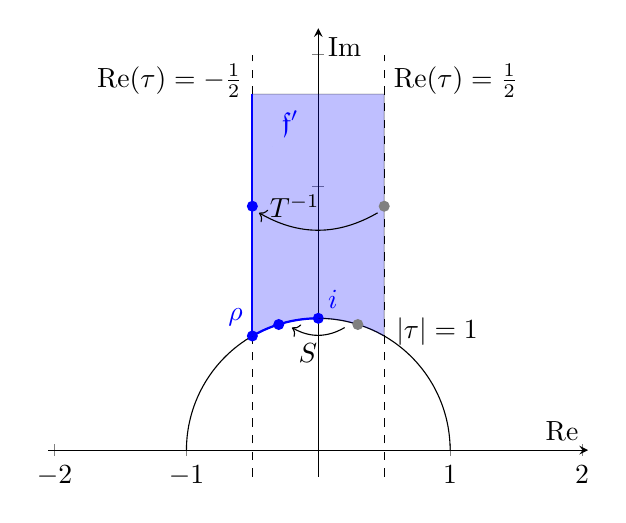
\begin{tikzpicture}
        \begin{axis}[
            axis lines=center,
            xlabel=$\text{Re}$,
            ylabel=$\text{Im}$,
            xmin=-1.5, xmax=1.5,
            ymin=-0.2, ymax=3.2, % Adjusted ymax
            axis equal,
            legend pos=outer north east,
            legend style={draw=none},
            yticklabels={$0$, $0$, , ,}
        ]
    
        % Draw x-axis and y-axis
        \draw[-] (axis cs: -1.5,0) -- (axis cs: 1.5,0) node[below right] {};
        
        % Draw y-axis with cutoff
        \ifnum\pdfstrcmp{\pgfkeysvalueof{/pgfplots/ymin}}{-0.2}>0
            \draw[-] (axis cs: 0,-0.2) -- (axis cs: 0,3) node[above left] {$y$};
        \fi
    
        % Draw semicircle
        \addplot[domain=0:180, samples=100, black] ({cos(x)}, {sin(x)});
        \node[black] at (axis cs: 0.9, 0.9) {$|\tau| = 1$};
    
        % Draw lines x=1/2 and x=-1/2 with cutoff
        \ifnum\pdfstrcmp{\pgfkeysvalueof{/pgfplots/xmin}}{-0.2}>0
            \draw[dashed] (axis cs: 0.5,-0.2) -- (axis cs: 0.5,3) node[below right] {$\text{Re}(\tau)=\frac{1}{2}$};
            \draw[dashed] (axis cs: -0.5,-0.2) -- (axis cs: -0.5,3) node[below left] {$\text{Re}(\tau)=-\frac{1}{2}$};
        \fi

        % Mark the point (0,1) and label it as i (changed coordinates)
        \fill[blue] (axis cs:0,1) circle[radius=2pt] node[above right,blue] {$i$};

        % Mark the point (-1/2, sqrt(3)/2) and label it as \rho
        \fill[blue] (axis cs:-0.5,{sqrt(3)/2}) circle[radius=2pt] node[above left,blue] {$\rho$};
    
        \coordinate (A) at (axis cs:0.5, 0.866);
        \coordinate (A2) at (axis cs:0.4, 0.916);
        \coordinate (A3) at (axis cs:0.3, 0.953);
        \coordinate (A4) at (axis cs:0.2, 0.9797);
        \coordinate (A5) at (axis cs:0.1, 0.99498);
        \coordinate (A6) at (axis cs:0, 1);
        \coordinate (A10) at (axis cs:-0.4, 0.916);
        \coordinate (A9) at (axis cs:-0.3, 0.953);
        \coordinate (A8) at (axis cs:-0.2, 0.9797);
        \coordinate (A7) at (axis cs:-0.1, 0.99498);
        \coordinate (B) at (axis cs:-0.5, 0.866);
        \coordinate (C) at (axis cs:-0.5, 2.7);
        \coordinate (D) at (axis cs:0.5, 2.7);

        % Draw the lines connecting the points
        \draw[fill=blue, opacity=0.25, name path=ABCD] (A) -- (A2) -- (A3) -- (A4) -- (A5) -- (A6) -- (A7) -- (A8) -- (A9) -- (A10) -- (B) -- (C) -- (D) -- cycle;

        \coordinate (B1) at (axis cs: -0.5, 0.866);
        \coordinate (B2) at (axis cs: -0.5, 2.7);
        \draw[blue, thick] (B1) -- (B2);

        \addplot[domain=90:120, samples=100, blue, thick] ({cos(x)}, {sin(x)});

        \coordinate (C1) at (axis cs: 0.45, 1.8);
        \coordinate (C2) at (axis cs: -0.45, 1.8);
        \fill[gray] (axis cs: 0.5, 1.85) circle[radius=2pt];
        \fill[blue] (axis cs: -0.5, 1.85) circle[radius=2pt];
        \draw[->, bend left=30] (C1) to node[pos = 0.7, above] {$T^{-1}$} (C2);

        \coordinate (D1) at (axis cs: 0.2, 0.9297);
        \coordinate (D2) at (axis cs: -0.2, 0.9297);
        \fill[gray] (axis cs: 0.3, 0.953) circle[radius=2pt];
        \fill[blue] (axis cs: -0.3, 0.953) circle[radius=2pt];
        \draw[->, bend left=30] (D1) to node[pos = 0.7, below] {$S$} (D2);

        \fill[blue] (axis cs:-0.35,2.3) circle[radius=0pt] node[above right,blue] {$\mathfrak{f}'$};

        \end{axis}
    \end{tikzpicture}    
\end{center}

\begin{prop}
    Let $G = \Gamma(1)/\{\pm I\}$. Then
    \begin{enumerate}[(i)]
        \item $\forall \tau \in \mathfrak{h}, \tau$ is $\Gamma(1)$--conjugate to an element of $\mathfrak{f}'$.
        \item If $\tau, \tau' \in \mathfrak{f}'$ are $\Gamma(1)$--conjugate, then $\tau = \tau'$.
        \item If $\tau \in \mathfrak{f'}$, then $\text{Stab}_G(\tau)$ is trivial, except in the two cases $\text{Stab}_G(i) = \langle S \rangle$ and $\text{Stab}_G(\rho) = \langle ST \rangle$, where $\rho = e^{2\pi i / 3}$.
        \item $\Gamma(1)$ is generated by $S$ and $T$.
    \end{enumerate}
\end{prop}
\begin{proof}
    Let $H$ be the subgroup of $G$ generated by $S$ and $T$.
    \begin{claim*}
        Every $\tau \in \mathfrak{h}$ is $H$--conjugate to an element of $\mathfrak{f}'$.
    \end{claim*}
    \begin{proof}
        By our above observation and since $S,T \in H$, it suffices to prove that every $\tau \in \mathfrak{h}$ is $H$--conjugate to $\mathfrak{f}$. Take $\tau \in \mathfrak{h}$. Recall that if $\gamma = \begin{pmatrix} a & b\\c &d \end{pmatrix} \in SL_2(\mathbb{Z})$, then $\text{Im}(\gamma \tau) = \frac{\text{Im}(\tau)}{|c \tau + d|^2}$. 
        \vspace{1mm}
         
        In particular, $\forall R \ge 0$, the intersection $H \tau \cap \{\text{Im}(\tau') > R\}$ is finite, since $\text{Im}(\gamma \tau) > R \iff |c \tau + d|^2 < \frac{\text{Im}(\tau)}{R}$, but $\Lambda_\tau = \mathbb{Z} \tau \oplus \mathbb{Z}$ is a lattice, so the set $\{(c,d) \in \mathbb{Z}^2 \mid |c \tau +d| < R'\}$ is finite. 
        \vspace{1mm}
         
        So there exists $h \in H$ such that $\text{Im}(h \tau) \ge \text{Im}(h' \tau) ~\forall h' \in H$. After replacing $\tau$ by $h \tau$, we can assume $\text{Im}(\tau) \ge \text{Im}(h \tau) ~\forall h \in H$. Since acting by $T$ does not change $\text{Im}(\tau)$, we can also assume $\text{Re}(\tau) \in \left[-\frac{1}{2},\frac{1}{2}\right]$. We have $\text{Im}(\tau) \ge \text{Im}(S \tau) = \frac{\text{Im}(\tau)}{|\tau|^2} \implies |\tau|\ge 1$, proving the claim and (i).
    \end{proof}
    Now take $\tau, \tau' \in \mathfrak{f}'$ and suppose $\gamma \tau = \tau'$ for some $\gamma = \begin{pmatrix} a & b \\ c & d \end{pmatrix} \in \Gamma(1)$. We want to show that either $\gamma = \pm I$ or $\tau = i, \rho$. 
    \vspace{1mm}
     
    WLOG assume $\text{Im}(\tau') = \text{Im}(\gamma \tau) \ge \text{Im}(\tau)$, i.e. $\text{Im}(\gamma \tau) = \frac{\text{Im}(\tau)}{|c \tau + d|^2} \ge \text{Im}(\tau)$, so $|c \tau +d| \le 1$. However, if $\tau \in \mathfrak{f}'$, then $\text{Im}(\tau) \ge \frac{\sqrt{3}}{2}$ with equality if and only if $\tau = \rho$. Hence $|c \tau + d| \ge |c| \text{Im}(\tau) \ge |c|\frac{\sqrt{3}}{2} \implies |c|\le \frac{2}{\sqrt{3}} \implies |c| = 0, 1 \implies c = 0$ or $c = \pm 1$. 
    \begin{itemize}
        \item If $c=0$, then $\gamma =\begin{pmatrix} a&b\\0&d \end{pmatrix}$, so $ad = 1 \implies a = d = \pm 1$, so $\gamma = \pm T^m$ for $m \in \mathbb{Z}$. However, $T$ acts on $\mathfrak{f}'$ by shifting the real part, so it can only stay in $\mathfrak{f}'$ if $m = 0$ (as $\text{Re}(\mathfrak{f}') \in \left[-\frac{1}{2},\frac{1}{2}\right)$), so $\gamma = \pm I$ and $\tau' = \tau$.
        \item If $c=1$, then $\gamma = \begin{pmatrix} a & b\\1 & d \end{pmatrix}$ and $|\tau +d|\le 1$. By drawing another picture, we see that the only circles centered at integers of radius 1 which intersect $\mathfrak{f}'$ are centered at $-d = 0, -d = -1$. Hence either $d = 0$, whence $|\tau|=1$, or $d=1$, whence $\tau = \rho$.
        \begin{itemize}
            \item If $c=1, d= 0, |\tau|=1$, then $\gamma = \begin{pmatrix} a & b \\ 1& 0 \end{pmatrix} = \begin{pmatrix} a & -1 \\ 1 & 0 \end{pmatrix}$ since the determinant must be 1. Then $\gamma \tau =  \frac{a \tau - 1}{\tau} = a -\frac{1}{\tau} = a - \overline{\tau}$, so $\text{Re}(\gamma\tau) = a - \text{Re}(\tau) \in \text{Re}(\mathfrak{f}' \cap \{|\tau|=1\}) = \left[-\frac{1}{2}, 0\right]$. However, we also have $\text{Re}(\gamma \tau) \in a - \left[-\frac{1}{2},0\right] = a + \left[0,\frac{1}{2}\right]$. \vspace{1mm}
             
            The intersection $\left[-\frac{1}{2}, 0 \right] \cap \left(a + \left[0, \frac{1}{2}\right]\right)$ can be nonempty only if either $a=0$, whence $\text{Re}(\gamma \tau) = \text{Re}(\tau) = 0$, so $\tau = \gamma \tau = i$, or $a = -1$, whence $\text{Re}(\tau) = \text{Re}(\gamma \tau) = -\frac{1}{2}$, so $\tau = \gamma \tau = \rho$. 
            \vspace{1mm}
             
            If $a=0$, then $\gamma = \begin{pmatrix} 0  & -1 \\ 1 & 0 \end{pmatrix} = -S$, which stabilizes $i$, and $\langle -S \rangle = \langle S \rangle$.
            \vspace{1mm}
             
            If $a=-1$, then $\gamma = \begin{pmatrix} -1 & -1 \\ 1 & 0 \end{pmatrix} = (ST)^2$, which stabilizes $\rho$, and $(ST)^3 = I$, so $\langle (ST)^2 \rangle = \langle ST \rangle$.
            \item If $c=1, d=1, \tau = \rho$, then $\gamma = \begin{pmatrix} a & b \\1 & 1 \end{pmatrix}$, so $\rho = \gamma \rho = \frac{a \rho + b}{\rho + 1}$. We have $\rho^2 + \rho + 1 = 0$, so $\rho^2 + \rho = -1$, so $a \rho + b = \rho^2 + \rho = -1$. But $a, b \in \mathbb{Z}$ and $1,\rho$ are linearly independent over $\mathbb{R}$, so $a = 0, b = -1$, so $\gamma = \begin{pmatrix} 0 & -1 \\ 1 & 1 \end{pmatrix} = -ST$, which stabilizes $\rho$.
        \end{itemize}
        \item If $c = -1$, we can reduce this to the case $c=1$ by replacing $\gamma$ with $-\gamma$.
    \end{itemize}
    We have now shown the first three parts of the proposition. It remains to show the last part, i.e. $\Gamma(1) = \langle S,T \rangle$. Since $S^2 = -I$, it is enough to show that $H = G$. Choose $\tau \in \text{Int}(f)$, so $\text{Stab}_G(\tau) = \{I\}$. Let $g \in G$. By our claim proving (i), $\exists h \in H$ such that $hg \tau  \in \mathfrak{f}'$. We must therefore have $hg \tau = \tau$, hence $h g  \in \text{Stab}_G(\tau) = \{I\}$, so $g = h^{-1} \in H$.
\end{proof}

\marginpar{13 Oct 2022, Lecture 4}

\textbf{Notation.} We write $e_{\tau} = |\text{Stab}_G(\tau)|$.
\vspace{1mm}
 
Let $f$ be a nonzero modular function of weight $k$, level $\Gamma(1)$. If $\tau \in \mathfrak{h}$, then $v_{\tau}(f)$ is the order of $f$ at $\tau$ (the unique $n \in \mathbb{Z}$ such that $f(z) = (z-\tau)^n g(z)$ for some meromorphic $g$ that is holomorphic and non--vanishing at $\tau$). We define $v_{\infty}(f)$ to be the order of $f$ at infinity, i.e. $v_{\infty}(f)=v_0(\tilde{f})$ for $\tilde{f}$ the meromorphic function in $D(0,1)$ with $f(\tau) = \tilde{f}(e^{2\pi i \tau})$.

\begin{prop}
    Let $f$ be a nonzero modular function of weight $k$, level $\Gamma(1)$. Then 
    \begin{align*}
        \sum_{ \tau \in \Gamma(1)\setminus \mathfrak{h}}^{} \frac{1}{e_{\tau}}v_\tau(f) + v_\infty(f) = \frac{k}{12}.
    \end{align*}
\end{prop}
\begin{proof}
    We first check that the sum is well--defined: 
    \begin{itemize}
        \item If $\tau \in \mathfrak{h}$, then $e_\tau, v_{\tau}(f)$ only depend on the $\Gamma(1)$--orbit of $\tau$. This is because if $\gamma \in \Gamma(1)$ and $\tau \in \mathfrak{h}$, then $\text{Stab}_{\Gamma(1)}(\tau)$ and $\text{Stab}_{\Gamma(1)}(\gamma \tau)$ are conjugate subgroups of $\Gamma(1)$, so $e_{\tau} = e_{\gamma \tau}$. On the other hand, $f(\gamma \tau) = f(\tau) j(\gamma, \tau)^k$ and $j(\gamma, \tau)$ is holomorphic and non--vanishing on $\mathfrak{h}$, so $v_{\gamma \tau}(f) = v_{\tau}(f)$.
        \item The sum only has a finite number of nonzero terms, since if $f$ is a modular function and $\tilde{f}$ is a meromorphic function on $D(0,1)$, then $\exists \delta > 0$ such that $\tilde{f}$ is holomorphic and non--vanishing in $D^*(0,\delta)$. Thus $\exists R > 0$ such that $f$ is holomorphic and non--vanishing in $\{\tau \in \mathfrak{h} \mid \text{Im}(\tau)>R\}$. Hence to show the sum is finite, it suffices to show that $f$ only has a finite number of zeroes and poles in $\mathfrak{f}$ (as $\mathfrak{f}$ intersects every $\Gamma(1)$--orbit), for which it suffices to show that $f$ has a finite number of zeroes and poles in $\mathfrak{f} \cap \{\tau \in \mathfrak{h} \mid  \text{Im}(\tau)\le R\}$, which is true as the set is compact (closed and bounded) and the zeroes and poles of $f$ are discrete.
    \end{itemize}
    To prove the identity, we use contour integration. Setup: if $U \subset \mathbb{C}$ is an open subset, $f : U \to \mathbb{C}$ is holomorphic and $\gamma:[0,1] \to U$ is a path, then $$\int_{\gamma}^{} f(z)\mathrm{d}z = \int_{t=0}^{1} f(\gamma(t))\gamma'(t)\mathrm{d}t.$$ We have the pullback formula: if $u : U \to V$ is a holomorphic map between open subsets of $\mathbb{C}$, $g : V \to \mathbb{C}$ is holomorphic and $\gamma$ is a path in $U$, then $$\int_{u \circ \gamma}^{} g(z)\mathrm{d}z = \int_{\gamma}^{} u^*(g(z)\mathrm{d}z) = \int_{\gamma}^{} g(u(z))u'(z)\mathrm{d}z.$$ A particularly nice case: if $g(z)=h'(z)/h(z)$, then $g(z)\mathrm{d}z = d \log h$, so $\int_{u \circ \gamma}^{}d \log h = \int_{\gamma}^{} u^*(d \log h) = \int_{\gamma}^{} d(\log h \circ u) = \int_{\gamma}^{} \frac{(h \circ u)'(z)}{(h \circ u)(z)}\mathrm{d}z$.
    \vspace{1mm}
     
    We also have (Cauchy's) argument principle: if $U \subset \mathbb{C}$ is a simply connected open subset, $\gamma \subset U$ is a simple positvely oriented closed path and $g$ is a meromorphic function in $U$ with no zeroes or poles on $\gamma$, then $$\frac{1}{2\pi i} \oint_{\gamma} d \log g = \frac{1}{2\pi i} \oint_{\gamma} \frac{g'(z)}{g(z)}\mathrm{d}z = \sum_{a \in \text{Int}(\gamma)}^{} v_a(g).$$
    We now apply this to our modular function $f$. Choose $R>0$ such that $f$ has no zeroes or poles in $\{\tau \in \mathfrak{h} \mid \text{Im}(\tau)\ge R\}$. We consider $\frac{1}{2\pi i}\oint_{\gamma} d \log f$, where $\gamma$ is the contour $ABCDE$.
    
    \begin{center}
        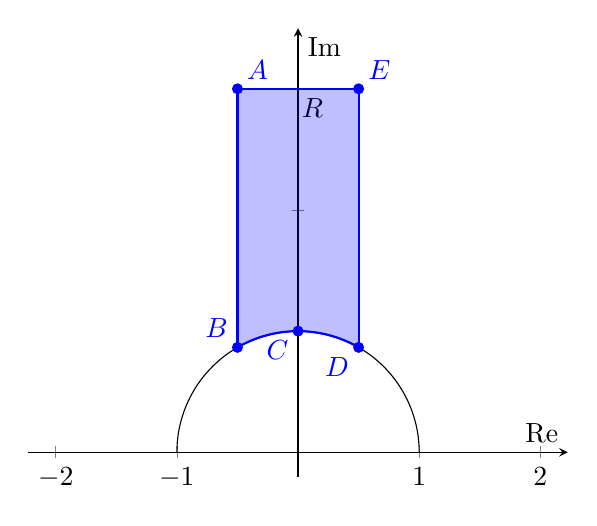
\begin{tikzpicture}
            \begin{axis}[
                axis lines=center,
                xlabel=$\text{Re}$,
                ylabel=$\text{Im}$,
                xmin=-1.5, xmax=1.5,
                ymin=-0.2, ymax=3.5, % Adjusted ymax
                axis equal,
                legend pos=outer north east,
                legend style={draw=none},
                yticklabels={$0$, $0$, , ,$R$},
                yticklabel style={below right},
            ]
        
            % Draw x-axis and y-axis
            \draw[-] (axis cs: -1.5,0) -- (axis cs: 1.5,0) node[below right] {};
            
            % Draw y-axis with cutoff
            \ifnum\pdfstrcmp{\pgfkeysvalueof{/pgfplots/ymin}}{-0.2}>0
                \draw[-] (axis cs: 0,-0.2) -- (axis cs: 0,3) node[above left] {$y$};
            \fi
        
            % Draw semicircle
            \addplot[domain=0:180, samples=100, black] ({cos(x)}, {sin(x)});
            \node[black] at (axis cs: 0.9, 0.9) {};
        
            % Draw lines x=1/2 and x=-1/2 with cutoff
            % \ifnum\pdfstrcmp{\pgfkeysvalueof{/pgfplots/xmin}}{-0.2}>0
            %     \draw[dashed] (axis cs: 0.5,-0.2) -- (axis cs: 0.5,2.8) node[below right] {$\text{Re}(\tau)=\frac{1}{2}$};
            %     \draw[dashed] (axis cs: -0.5,-0.2) -- (axis cs: -0.5,2.8) node[below left] {$\text{Re}(\tau)=-\frac{1}{2}$};
            % \fi
    
            % Mark the point (0,1) and label it as i (changed coordinates)
            \fill[blue] (axis cs:-0.5,3) circle[radius=2pt] node[above right,blue] {$A$};

            \fill[blue] (axis cs:0.5,3) circle[radius=2pt] node[above right,blue] {$E$};
            
            \fill[blue] (axis cs:0,1) circle[radius=2pt] node[below left,blue] {$C$};
    
            % Mark the point (-1/2, sqrt(3)/2) and label it as \rho
            \fill[blue] (axis cs:-0.5,{sqrt(3)/2}) circle[radius=2pt] node[above left,blue] {$B$};

            \fill[blue] (axis cs:0.5,{sqrt(3)/2}) circle[radius=2pt] node[below left,blue] {$D$};
        
            \coordinate (A) at (axis cs:0.5, 0.866);
            \coordinate (A2) at (axis cs:0.4, 0.916);
            \coordinate (A3) at (axis cs:0.3, 0.953);
            \coordinate (A4) at (axis cs:0.2, 0.9797);
            \coordinate (A5) at (axis cs:0.1, 0.99498);
            \coordinate (A6) at (axis cs:0, 1);
            \coordinate (A10) at (axis cs:-0.4, 0.916);
            \coordinate (A9) at (axis cs:-0.3, 0.953);
            \coordinate (A8) at (axis cs:-0.2, 0.9797);
            \coordinate (A7) at (axis cs:-0.1, 0.99498);
            \coordinate (B) at (axis cs:-0.5, 0.866);
            \coordinate (C) at (axis cs:-0.5, 3);
            \coordinate (D) at (axis cs:0.5, 3);
            \coordinate (E) at (axis cs:0.5, 3);
    
            % Draw the lines connecting the points
            \draw[fill=blue, opacity=0.25, name path=ABCD] (A) -- (A2) -- (A3) -- (A4) -- (A5) -- (A6) -- (A7) -- (A8) -- (A9) -- (A10) -- (B) -- (C) -- (E) -- (D) -- cycle;
    
            \coordinate (B1) at (axis cs: -0.5, 0.866);
            \coordinate (B2) at (axis cs: -0.5, 3);
            \draw[blue, thick] (B1) -- (B2) -- (E) -- (A);
                
            
            \addplot[domain=60:120, samples=100, blue, thick] ({cos(x)}, {sin(x)});    
            \end{axis}
        \end{tikzpicture}    
    \end{center}

    By choice of $R$, there are no zeroes or poles of $f$ on $AE$. We first consider the case where $f$ has no zeroes or poles at all on $\gamma$. Then the argument principle gives $$\frac{1}{2\pi i}\oint_{\gamma} d \log f = \frac{1}{2\pi i} \int_{AB}^{} +\int_{BC}^{} +\int_{CD}^{} +\int_{DE}^{} +\int_{EA}^{} d \log f = \sum_{\tau \in \Gamma(1)\setminus \mathfrak{h}}^{} \frac{1}{e_{\tau}}v_\tau(f) $$
    (as $v_\tau(f) \neq 0$, $e_{\tau} = 1$ under our assumptions).
    \vspace{1mm}
     
    Apply the pullback formula with $u(\tau) = \tau+1$. Then $u(AB) = ED$, $f \circ u = f$, so $$\int_{u(AB)}^{} d \log f = \int_{AB}^{} d \log f \circ u = \int_{AB}^{} d \log f = \int_{ED}^{} d \log f = - \int_{DE}^{} d \log f.$$
    Hence $\int_{AB}^{} + \int_{DE}^{} d \log f = 0$.
    \vspace{1mm}
     
    Now take $q = e^{2\pi i \tau}$, so $f = \tilde{f} \circ q$ and $q(AE)$ is a positively oriented circle around 0 in $D(0,1)$. So $$\frac{1}{2\pi i} \int_{q(AE)}^{} d \log \tilde{f} = v_{\infty}(f) = \frac{1}{2\pi i} \int_{AE}^{} d \log \tilde{f} \circ q = \frac{1}{2\pi i}\int_{AE}^{} d \log f.$$ 
    \vspace{1mm}
     
    Now take $v(\tau) = S(\tau) = -\frac{1}{\tau}$. Then $v(BC) = DC$ and we know $f|_k[S](\tau) = f\left(-\frac{1}{\tau}\right)\tau^{-k} = f(\tau)$, so $f \circ v = f(\tau)\tau^k$. Hence 
    \begin{align*}
        &\int_{DC}^{} d \log f = \int_{v(BC)}^{} d \log f = \int_{BC}^{} d \log (f \circ v) = \int_{BC}^{} d \log(f(\tau)\tau^k) \\ =& \int_{BC}^{} d \log f + k d \log \tau = \int_{BC}^{} d \log f + k(\log C - \log B)
    \end{align*}
    where here $\log$ is any branch of the logarithm defined on $BC$. But $B = \rho, C = i$, so $\log B = i \frac{2\pi}{3}$ and $\log C = i \frac{\pi}{2}$. Hence \[
    \int_{CD}^{} d \log f = - \int_{DC}^{} d \log f + k\left(\frac{2\pi i }{3} - \frac{2 \pi i }{4}\right),
    \]
    giving \[
    \int_{BC}^{} +\int_{CD}^{} d \log f = 2\pi i k \frac{1}{12}.
    \]
    We have 
    \begin{align*}
        \sum_{\Gamma(1)\setminus \mathfrak{h}}^{} \frac{1}{e^{\tau}} v_\tau(f) =& \frac{1}{2\pi i } \left(\int_{AB}^{} +\int_{BC}^{} +\int_{CD}^{} +\int_{DE}^{} +\int_{EA}^{} d \log f \right) \\
        =& \frac{1}{2\pi i} \left( 0 + \frac{k}{12} + 0 - v_{\infty}(f) \right) \\
        &\implies \sum_{ \tau \in \Gamma(1)\setminus \mathfrak{h}}^{} \frac{1}{e_{\tau}}v_\tau(f) + v_\infty(f) = \frac{k}{12}.
    \end{align*}
    This finishes the proof in the case where there are no zeroes or poles. If there are zeroes or poles on $\gamma$, we need to modify the contour. For example, if there's a zero or a pole at a point $P$ on $AB$, then consider the contour $\gamma'$, which is just $\gamma$ but with a small semicircle around our (discrete) pole, which satisfies the property that $f$ has no zeroes or poles on $\gamma'$. The trickiest case is when there is a zero or pole at $B = \rho$ or $C = i$. This is Q3 on example sheet 1. 
\end{proof}

\marginpar{16 Oct 2022, Lecture 5}

\begin{example}
    Take $k=4$, $f = E_4 \in M_{4}(\Gamma(1))$. Hence $\forall \tau \in \mathfrak{h}, v_{\tau}(E_4)\ge 0$ (as it is holomorphic in $\mathfrak{h}$). We know $E_4(\tau) = 1 + \sum_{n\ge 1}^{} a_nq^n$, so $E_4(\infty) \neq 0$ and $v_{\infty}(E_4) = 0$. Hence our formula gives 
    \begin{align*}
        \sum_{\tau \in \Gamma(1)\setminus \mathfrak{h}}^{} \frac{1}{e_{\tau}}v_{}(E_4) = \frac{1}{3} v_{\rho}(E_4) + \frac{1}{2}v_i(E_4) + \sum_{\tau \in \Gamma(1)\setminus \mathfrak{h}, \tau \not\sim \rho,i}^{} v_{\tau}(E_4) = \frac{1}{3}.
    \end{align*}
    So we have $\frac{a}{3}+\frac{b}{2}+c = \frac{1}{3}$, where $a,b,c \in \mathbb{Z}_{\ge 0}$, which gives the only solution $a=1, b=c=0$, so $E_4(\rho)=0$ and $E_4(\tau) \neq 0$ if $\tau \not\in \Gamma(1)\rho$.
    \vspace{1mm}
     
    If $k=6$, $f = E_6$, then we get \[
    \frac{1}{3}v_{\rho}(E_6) + \frac{1}{2}v_i(E_6) + \sum_{\tau \not\sim \rho,i}^{} v_{\tau}(E_6) = \frac{6}{12} = \frac{1}{12},
    \]
    so this forces $v_{\rho}(E_6) = 0$, $v_{i}(E_6) = 1$, $v_{\tau}(E_6) \neq 0$ if $\tau \not\sim \rho$ and $\tau \not\sim i$, so $E_6(i) = 0$, $E_6(\tau) \neq 0$ if $\tau \not\sim \rho,i$.
\end{example}
Recall $\Delta = \frac{E_4^3 - E_6^2}{1728} \in S_{12}(\Gamma(1))$. This is nonzero since $\Delta(\rho) = \frac{E_4(\rho)^3 - E_6(\rho)^2}{1728}  = -\frac{E_6(\rho)^2}{1728} \neq 0$. We also have $v_{\infty}(\Delta)\ge 1$ by construction, so plug in $\Delta$ to our formula to get 
\begin{align*}
    \sum_{\tau}^{} \frac{1}{e_{\tau}}v_{\tau}(\Delta) + v_{\infty}(\Delta) = 1,
\end{align*}
so $v_{\infty}(\Delta) = 1$, so $\Delta$ has a simple zero at $\infty$ and $\Delta$ is nonvanishing in $\mathfrak{h}$.

\begin{theorem}
    Let $k \in 2\mathbb{Z}$. Then:
    \begin{enumerate}[(1)]
        \item If $k<0$ or $k=2$, then $M_k(\Gamma(1)) = 0$; and $M_0(\Gamma(1)) = \mathbb{C} \cdot 1$.
        \item If $4\le k\le 10$, then $M_k(\Gamma(1)) = \mathbb{C} \cdot E_k$. 
        \item For any $k$, multiplication by $\Delta$ gives an isomorphism $M_k(\Gamma(1)) \stackrel{\times \Delta}{\to}  S_{k+12}(\Gamma(1))$.
    \end{enumerate}
\end{theorem}
\begin{proof}
    \begin{enumerate}[(1)]
        \item Let $f \in M_k(\Gamma(1))$ be nonzero. Then $\sum_{}^{} \frac{1}{e_{\tau}}v_{\tau}(f) + v_{\infty}(f) = \frac{k}{12}$. Note the LHS is $\ge 0$, but for $k<0$, the RHS is $<0$. If $k=2$, then we get the equation $\frac{a}{3}+\frac{b}{2}+c = \frac{1}{6}$ for $a,b,c \in \mathbb{Z}_{\ge 0}$, which has no solutions.
        \vspace{1mm}
         
        Suppose $f \in M_0(\Gamma(1)) \setminus \mathbb{C}\cdot 1$. Then $f - f(\infty) \cdot 1  \in S_0(\Gamma(1))$ is a nonzero function (here 1 is the constant function 1). Then $\sum_{\tau}^{} \frac{1}{e_{\tau}}v_{\tau}(f-f(\infty)\cdot 1) + \underbrace{v_{\infty}(f-f(\infty)\cdot 1)}_{\ge 1} = 0$, a contradiction, so $M_0(\Gamma(1)) = \mathbb{C}\cdot 1$.
        \item Let $4\le k\le 10$ and $f \in M_k(\Gamma(1))$. Consider $f - f(\infty)\cdot E_k \in S_k(\Gamma(1))$. If this is nonzero, then \[
        \sum_{\tau}^{} \frac{1}{e_\tau}v_{\tau}(f-f(\infty)\cdot E_k) + \underbrace{v_{\infty}(f-f(\infty)\cdot E_k)}_{\ge 1} = \frac{k}{12}<1,
        \]
        a contradiction. So $f = f(\infty)\cdot E_k$.
        \item Our map $\times \Delta : M_k(\Gamma(1)) \to S_{k+12}(\Gamma(1))$ is a well--defined $\mathbb{C}$--linear map. It is injective, since if $\Delta f = 0$, then $f = 0$ (as $\Delta$ is nonvanishing in $\mathfrak{h}$). For surjectivity, if $f \in S_{k+12}(\Gamma(1))$, then $\frac{f}{\Delta}$ is holomorphic in $\mathfrak{h}$ and invariant under the weight $k$ action of $\Gamma(1)$. 
        \vspace{1mm}
         
        We need to show $\frac{f}{\Delta}$ is holomorphic at $\infty$, as then $\frac{f}{\Delta} \in M_k(\Gamma(1))$, so $f = \frac{f}{\Delta}f \in \text{Im}(\times \Delta)$. Hence we need $v_{\infty}\left(\frac{f}{\Delta}\right) \ge 0$. But $v_{\infty}\left(\frac{f}{\Delta}\right) = \underbrace{v_{\infty}(f)}_{\ge 1} - \underbrace{v_{\infty}(\Delta)}_{=1} \ge 0$, so we're done.
    \end{enumerate}
\end{proof}
\begin{cor}
    If $k \in 2\mathbb{Z}$, $k\ge 0$, then $M_k(\Gamma(1))$ is finite--dimensional and $$\text{dim}_{\mathbb{C}}M_k(\Gamma(1)) = \begin{cases}
        \left\lfloor \frac{k}{12} \right\rfloor + 1 & k \not\equiv 2 \pmod{12}.\\
        \left\lfloor \frac{k}{12} \right\rfloor & k \equiv 2 \pmod{12}.
    \end{cases}$$
\end{cor}
\begin{proof}
    We proved this for $0\le k \le 10$. In general, use induction on $k$: we need to show that for $k\ge 0$, $\text{dim}_{\mathbb{C}}M_{k+12}(\Gamma(1)) = \text{dim}_{\mathbb{C}}M_k(\Gamma(1)) + 1$.
    \vspace{1mm}
     
    We know $E_{k+12} \in M_{k+12}(\Gamma(1))$, so $M_{k+12}(\Gamma(1)) = \mathbb{C} E_{k+12} \oplus S_{k+12}(\Gamma(1))$. But this equals $\mathbb{C} E_{k+12} \oplus \Delta M_k(\Gamma(1))$, so $\text{dim}_{\mathbb{C}} M_{k+12}(\Gamma(1)) = 1 + \text{dim}_{\mathbb{C}}M_k(\Gamma(1))$.
\end{proof}
\begin{example}
    We have $E_4^2 \in M_8(\Gamma(1)) = \mathbb{C} E_8$. So there is a relation between $E_4^2$ and $E_8$ (in this case, one is a scalar multiple of the other), but we have $E_8(\infty) = 1 = E_4(\infty)^2 \implies E_4^2 = E_8$.
    \vspace{1mm}
     
    Similarly, $E_4E_6 \in M_{10}(\Gamma(1)) = \mathbb{C} E_{10}$, so we find  $E_4 E_6 = E_{10}$.
\end{example}
\begin{cor}
    If $k \in 2\mathbb{N}$, then $M_k(\Gamma(1))$ is spanned as a $\mathbb{C}$--vector space by $\{E_4^aE_6^b \mid a,b \in \mathbb{Z}_{\ge 0}, 4a+6b=k\}$. In other words, if $\mathcal{M} = \oplus_{k \in \mathbb{Z}}M_k(\Gamma(1))$, then $\mathcal{M}$ is a graded $\mathbb{C}$--algebra generated by $E_4$ and $E_6$.
\end{cor}
\begin{proof}
    We proved this for $0\le k\le 10$. If $k\ge 12$, then $$M_k(\Gamma(1)) = \mathbb{C} E_k \oplus \Delta M_{k-12}(\Gamma(1)) = \mathbb{C} f \oplus \Delta M_{k-12}(\Gamma(1))$$ for any $f \in M_k(\Gamma(1))$ such that $f(\infty) \neq 0$ by the same argument. We can always find some $A,B \in \mathbb{Z}_{\ge 0}$ such that $4A+6B = k$, so $E_4^A E_6^B \in M_k(\Gamma(1))$ and $(E_4^A E_6^B)(\infty) \neq 0$. Now by induction, $M_{k-12}(\Gamma(1)) = \langle E_4^a E_6^b \mid 4a+6b = k-12 \rangle$, so $\Delta M_{k-12}(\Gamma(1)) = \langle \Delta E_4^a E_6^b \mid 4a+6b = k -12 \rangle$. But $\Delta \in \langle E_4^3, E_6^2 \rangle$, so \[
    \Delta M_{k-12}(\Gamma(1)) = \langle E_4^a E_6^b \mid 4a+6b = k \rangle
    \]
    and $E_4^A E_6^B \in \langle E_4^a E_6^b \mid 4a+6b = k \rangle$, so $M_k(\Gamma(1)) = \langle E_4^a E_6^b \mid 4a+6b = k \rangle$.
\end{proof}
\begin{theorem}
    Let $j(\tau) = \frac{E_4(\tau)^3}{\Delta}$. Then $j$ is a modular function of weight $0$, level $\Gamma(1)$ which is holomorphic on $\mathfrak{h}$ and has a simple pole at $\infty$. It defines a bijection $\Gamma(1)\setminus \mathfrak{h} \to \mathbb{C}$ given by $\tau \to j (\tau)$. Moreover, every modular function of weight 0, level $\Gamma(1)$ is a rational function of $j$.\footnote{Remember that $\Gamma(1)\setminus \mathfrak{h}$ is the set of orbits of $\Gamma(1)$ under $\mathfrak{h}$.}
\end{theorem}
The interpretation of this is that it is possible to define a Riemann surface structure on $\Gamma(1)\setminus \mathfrak{h} \sqcup \{\infty\}$ such that we get a compact Riemann surface whose meromorphic functions are exactly the modular functions of weight 0. So the theorem says that this Riemann surface, called $X(1)$, is isomorphic to the Riemann sphere, and our formula says that if $\mathcal{L}$ is an invertible sheaf on a compact Riemann surface and $S$ is a meromorphic section, then $\sum_{a}^{} v_a(S) = \text{deg}(\mathcal{L})$. This is useful if we are also taking algebraic geometry.

\marginpar{18 Oct 2022, Lecture 6}

\begin{proof}
    We showed that $\Delta$ is nonvanishing in $\mathfrak{h}$ and has a simple zero at $\infty$. Hence $j$ is holomorphic in $\mathfrak{h}$ and $v_{\infty}(j)=3v_{\infty}(E_4)-v_{\infty}(\Delta) = -1$. Note that if $\gamma \in \Gamma(1)$, then $j|_0[\gamma](\tau) = j(\gamma \tau) = j(\tau)$ since the map is constant on $\Gamma(1)$--orbits. To show the map is a bijection, we need to show that $\forall z \in \mathbb{C}$, there exists a unique orbit $\Gamma(1)\cdot \tau$ such that $j(\tau)=z$, i.e. $v_\tau(j-z)>0$. \vspace{1mm}
     
    We know \[
    \sum_{\tau \in \Gamma(1)\setminus \mathfrak{h}}^{} \frac{1}{e_{\tau}} \underbrace{v_{\tau}(j-z)}_{\ge 0, \text{ as }j-z \text{ is holomorphic in }\mathfrak{h}.} = 1,
    \]
    (since $v_{\infty}(j-z) = -1$ and $\frac{k}{12}= 0$) again giving $\frac{a}{3} +\frac{b}{2}+c= 1$ for $a,b,c \in \mathbb{Z}_{\ge 0}$, $ a = v_{\rho}(j-z), b = v_{i}(j-z), c = \sum_{\tau \not\sim \rho,i}^{} v_\tau(j-z)$. This gives the solutions 
    \begin{itemize}
        \item $(a,b,c) = (0,0,1)$, so $j-z$ vanishes at a unique $\Gamma(1)\cdot \tau$.
        \item $(a,b,c) = (0,2,0)$, so $j-z$ vanishes at $i$.
        \item $(a,b,c) = (3,0,0)$, so $j-z$ vanishes at $\rho$.
    \end{itemize}
    Hence our map is bijective. Consider a nonzero modular function $f$ of weight 0. To get rid of all the poles, we can consider a product $f \cdot \prod_{i=0}^{n} \left(j(\tau)-j(a_i)\right)^{b_i}$ for $a_i \in \mathfrak{h}$, $b_i \in \mathbb{Z}_{\ge 0}$, where the $a_i$ are among the poles of $f$ in $\mathfrak{h}$. Hence to show $f$ is a rational function of $j$, it is enough to consider the case where $f$ is holomorphic in $\mathfrak{h}$. Then there exists $m\ge 0$ such that $\Delta^m f$ is holomorphic at $\infty$, so $\Delta^m f$ is holomorphic in $\mathfrak{h}$ and at $\infty$, so $\Delta^m f \in M_{12m}(\Gamma(1))$. We showed that $M_{12m}(\Gamma(1)) = \langle E_4^a E_6^b \mid 4a+6b=12m \rangle$, so $f$ is a linear combination of functions of the form $\frac{E_4^aE_6^b}{\Delta^m}$, where $4a+6b=12m$. 
    \vspace{1mm}
     
    Hence it is enough to show that $\frac{E_4^aE_6^b}{\Delta^m}$ is a rational function of $j$ where $4a+6b=12m$, $a,b \in \mathbb{Z}_{\ge 0}$. But then $2a+3b=6m$, which gives $p,q \in \mathbb{\mathbb{Z}}_{\ge 0}$ such that $a =3p, b = 2q$, so $p+q=m$. Then $$\frac{E_4^aE_6^b}{\Delta^m} = \left(\frac{E_4^3}{\Delta}\right)^p \left(\frac{E_6^2}{\Delta}\right)^q = j^p \left(\frac{E_6^2}{\Delta}\right)^q.$$ 
    As $E_4^3 - E_6^2 = 1728\Delta$, we get $j = \frac{E_6^2}{\Delta} + 1728$. So this is a rational function of $j$.
\end{proof}
\begin{prop}
    Let $k\ge 4$ be an even integer. Then $$G_k(\tau) = 2\zeta(k) + 2\frac{(2\pi i)^k}{(k-1)!} \sum_{n\ge 1}^{} \sigma_{k-1}(n)q^n$$
    where $q = e^{2\pi i \tau}$ and $\sigma_{k-1}(n) = \sum_{d \mid n}^{} d^{k-1}$.
\end{prop}
\begin{proof}
    We start from the identity $$\pi \cot (\pi \tau) = \frac{1}{\tau} + \sum_{n\ge 1}^{} \left(\frac{1}{\tau+n} + \frac{1}{\tau-n}\right).$$
    This is true for $\tau \in \mathfrak{h}$ and it is even locally uniformly convergent in $\mathfrak{h}$. We can write \[
    \pi \cot(\pi \tau) = i\pi \frac{e^{\pi i \tau} + e^{-\pi i \tau}}{e^{\pi i \tau}-e^{- \pi i \tau}} = \pi i \frac{q+1}{q-1} = -\pi i (1+q)(1-q)^{-1} = -\pi i \left(1+2\sum_{n\ge 1}^{} q^n\right).
    \]
    Differentiate term--by--term $k-1$ times. The RHS of the bottom expression is \[
    -2\pi i \left(\frac{\mathrm{d}}{\mathrm{d}\tau}\right)^{k-1}\left(\sum_{n\ge 1}^{} q^n \right) = -\left(2\pi i\right)^k \sum_{n\ge 1}^{} n^{k-1}q^n,
    \]
    while the RHS of the top expression is \[
    (-1)^{k-1}(k-1)! \left(\tau^{-k} + \sum_{n\ge 1}^{} (\tau+n)^{-k} + (\tau-n)^{-k} \right) = (-1)^{k-1}(k-1)! \sum_{n \in \mathbb{Z}}^{} (\tau+n)^{-k}.   
    \]
    Rearranging and using the fact that $k$ is even (to make the sign go away) gives \[
    \sum_{n \in \mathbb{Z}}^{} (\tau+n)^{-k} = \frac{(2\pi i)^k}{(k-1)!} \sum_{n\ge 1}^{} n^{k-1}q^n, \tau \in \mathfrak{h}.
    \]
    Then \[
    G_k(\tau) = \sum_{(m,n) \in \mathbb{Z}^2\setminus 0}^{} (m \tau + n)^{-k} = 2 \zeta(k) + \sum_{\substack{(m,n) \in \mathbb{Z}^2\setminus 0, \\m \neq 0}}^{} (m \tau + n)^{-k} = 2 \zeta(k) + 2 \sum_{m\ge 1}^{} \sum_{n \in \mathbb{Z}}^{} (m \tau + n)^{-k}.
    \]
    Plug in our identity to get 
    \begin{align*}
        G_k(\tau) =& 2 \zeta(k) + \sum_{m\ge 1}^{} \frac{(2\pi i )^k}{(k-1)!} \sum_{n\ge 1}^{} n^{k-1}q^{mn} = 2\zeta(k) + \frac{2 (2\pi i)^k}{(k-1)!} \sum_{N\ge 1}^{} \underbrace{\left(\sum_{n \mid N}^{} n^{k-1}\right)}_{=\sigma_{k-1}(N)}q^N.
    \end{align*}
\end{proof}
\begin{cor}
    $E_k(\tau) = \frac{G_k(\tau)}{2\zeta(k)} = 1 + \sum_{n\ge 1}^{} a_nq^n$ has all $a_n \in \mathbb{Q}$. Moreover, if $k=4$ or $k=6$, then $a_n \in \mathbb{Z}$.
\end{cor}
\begin{proof}
    We have $$E_k(\tau) = 1 + \frac{(2\pi i)^k}{\zeta(k)(k-1)!}\sum_{n\ge 1}^{} \sigma_{k-1}(n)q^n.$$
    Hence we need to show that $\frac{\zeta(k)}{\pi^k}$ is rational. This is on example sheet 1 (when $k$ is even). One can show that $\zeta(4) = \frac{\pi^4}{90}$ and $\zeta(6) = \frac{\pi^6}{945}$, so 
    \begin{align*}
        &E_4(\tau) = 1 + \frac{2^4 \pi^4 \cdot 90}{\pi^4 \cdot 6}\sum_{n\ge 1}^{} \sigma_3(n)q^n = 1 + 240\sum_{n\ge 1}^{} \sigma_3(n)q^n\\
        &E_6(\tau) = 1 -\frac{2^6 \pi^6 \cdot 3^3 \cdot 5 \cdot 7}{\pi^6 \cdot 5!}\sum_{n\ge 1}^{} \sigma_5(n)q^n = 1 - 504 \sum_{n\ge 1}^{} \sigma_5(n)q^n.
    \end{align*}
\end{proof}
\begin{cor}
    If $\Delta(\tau) = \sum_{n\ge 1}^{} \tau(n)q^n$ is the $q$--expansion of $\Delta$, then $\tau(1)=1$ and $\tau(n) \in \mathbb{Z} ~\forall n\ge 1$.
\end{cor}
\begin{proof}
    Write $E_4 = 1 + 240U$ and $E_6 = 1 -504V$ for $U,V = q + \ldots \in \mathbb{Z}[[q]]$. Then 
    \begin{align*}
        \Delta &= \frac{E_4^3-E_6^2}{1728} = \frac{(1+240U)^3-(1-504V)^2}{1728} \\
        &= \frac{3\cdot 240U + 3\cdot 240^2 U^2 + 240^3 U^3 + 2\cdot 504V - 504^2V^2}{1728}\\
        &= \frac{(3\cdot 240 U + 2\cdot 504 V)}{1728} + R,
    \end{align*}
    where we claim $R \in q^2\mathbb{Z}[[q]]$, but for this we just need to check that $1728 \mid 3\cdot 240^2, 1728 \mid240^3, 1728 \mid504^2$, which is true.
    \vspace{1mm}
     
    We need to check that $$\frac{(3\cdot 240 U + 2\cdot 504 V)}{1728} = \frac{2^4 \cdot 3^2\cdot 5\cdot U + 2^4 \cdot 3^2\cdot 7\cdot V}{2^6\cdot 3^3} \in \mathbb{Z}[[q]].$$ But this equals \[
    \frac{5U+7V}{12} = \frac{5(U-V)}{12} + V.
    \]
    Hence we need to check that \[
    \frac{5}{12}(\sigma_3(n)-\sigma_5(n)) \in \mathbb{Z} ~\forall n\ge 1,
    \]
    i.e. we need to check that \[
    \sigma_3(n) \equiv \sigma_5(n) \pmod{12} ~\forall n\ge 1.
    \]
    But this is true as $d^3 \equiv d^5 \pmod{12} ~\forall d \in \mathbb{N}$.
    \vspace{1mm}
     
    Finally, we compute $\tau(1) =\frac{3\cdot 240 + 2\cdot 504}{1728} = 1$. 
\end{proof}

\marginpar{20 Oct 2022, Lecture 7}

\begin{theorem}
    Let $k\ge 4$ be even and $N = \text{dim}_{\mathbb{C}}~S_k(\Gamma(1))$. Then there exists a unique basis $f_0,\ldots,f_N$ for $M_k(\Gamma(1))$ as a $\mathbb{C}$--vector space such that
    \begin{enumerate}[(a)]
        \item $\forall 0\le i\le N$, $f_i = \sum_{n\ge 0}^{} a_n(f_i)q^n$ for $a_n(f_i) \in \mathbb{Z} ~\forall n\ge 0$.
        \item If $0\le i,n\le N$, then $a_n(f_i)=\delta_{in}$.
    \end{enumerate}
\end{theorem}
So in other words, $f_i = q^i + O(q^{N+1})$. This is important because $M_k(\Gamma(1))$ has a $\mathbb{Z}$--structure, i.e. we can realize it as a tensor product $M_k(\Gamma(1)) = M_k(\Gamma(1),\mathbb{Z})\oplus \mathbb{C}$, where $M_k(\Gamma(1),\mathbb{Z}) = \{f \in M_k(\Gamma(1)) \mid \forall n\ge 0, a_n(f) \in \mathbb{Z}\}$.

\begin{proof}
    We first construct $f_0,\ldots,f_N \in M_k(\Gamma(1))$ with properties (a) and (b). Write $k = 12a + d$, for $a, d \in \mathbb{Z}_{\ge 0}$ such that $d = 14$ if $k \equiv 2 \pmod{12}$, or $0\le d\le 10$ if $d \not\equiv 2 \pmod{12}$.
    \vspace{1mm}
     
    Then $$\left\lfloor \frac{k}{12} \right\rfloor = \begin{cases}
        a & k\not\equiv 2 \pmod{12}\\
        a+1 & k \equiv 2 \pmod{12}
    \end{cases} \implies \left\lfloor a\right\rfloor = \begin{cases}
        \left\lfloor \frac{k}{12} \right\rfloor & k\not\equiv 2 \pmod{12}\\
        \left\lfloor \frac{k}{12} \right\rfloor-1 & k \equiv 2 \pmod{12}.
    \end{cases}$$
    We have $\text{dim}_{\mathbb{C}}~M_k(\Gamma(1)) = N+1 = \begin{cases}
        \left\lfloor \frac{k}{12} \right\rfloor+1 & k \not\equiv 2 \pmod{12}\\
        \left\lfloor \frac{k}{12} \right\rfloor & k \equiv 2 \pmod{12},
    \end{cases}$ 
    so $a = N$, $k = 12N + d$.
    \vspace{1mm}
     
    Now consider $A, B \in \mathbb{Z}_{\ge 0}$ such that $d = 4A + 6B$. Consider the modular forms $$g_i = \Delta^i E_4^A E_6^B E_6^{2(N-i)}$$ for $0\le i\le N$. Each $g_i$ has weight $12i + 4A + 6B + 12(N-i) = 12N + d = k$, so $g_i \in M_k(\Gamma(1))$. As $E_4, E_6, \Delta$ have $q$--expansions in $\mathbb{Z}[[q]]$, so does $g_i$. The leading term of $g_i$ is $q^i$, so the $q$--expansions look like 
    \begin{align*}
        g_0 &= 1 + a_1(g_0)q + \ldots + a_N(g_0)q^N + O(q^{N+1})\\
        &\vdots\\
        g_{N-1} &= 0 + \ldots + q_{N-1} + a_N(g_{N-1})q^N + O(q^{N+1})\\
        g_N &= 0 + \ldots + 0 + q^N + O(q^{N+1})
    \end{align*}
    We can now carry out row reduction on the $g_i$ to obtain $f_0,\ldots,f_N$ satisfying (a) and (b). For uniqueness, consider the linear functionals 
    \begin{align*}
        &a_0,\ldots,a_N : M_k(\Gamma(1)) \to \mathbb{C}\\
        &f \mapsto a_i(f), ~f = \sum_{n\ge 0}^{} a_n(f)q^n.
    \end{align*}
    Then $a_i(f_j) = \delta_{ij}$, which forces $a_0,\ldots,a_n$ to be linearly independent. Hence they form a basis of the dual vector space $M_k(\Gamma(1))^{*}$. So $f_0,\ldots,f_N$ is the dual basis of $M_k(\Gamma(1))$, and they form the unique basis with this property.
\end{proof}

\section{Hecke operators}

Hecke operators are just symmetries (linear endomorphisms) of spaces of modular forms. They can arise from either representation theory: $\Gamma(1) \le GL_2(\mathbb{Q})^{+}$, which acts on $\{f : \mathfrak{h} \to \mathbb{C}\}$ by $f \mapsto f|_k[g]$. But $M_k(\Gamma(1)) \le \{f : \mathfrak{h} \to \mathbb{C}\}^{\Gamma(1)}$, and a general group theory fact says that under suitable conditions, there's an action by a big class of operators; or from geometry: we can think of modular forms as functions on the set of lattices $\mathcal{L}$ in $\mathbb{C}$. In this course, we will follow the second point of view.
\vspace{1mm}
 
\textbf{Recall.} If $V$ is a finite--dimensional $\mathbb{R}$--vector space, then a lattice $\Lambda$ in $V$ is a subgroup $\Lambda \subset V$ which is discrete and cocompact (i.e. $V/\Lambda$ is compact).

\begin{lemma}
    A subgroup $\Lambda \le V$ is a lattice if and only if there exists a basis $e_1,\ldots,e_n$ for $V$ as a $\mathbb{R}$--vector space such that $\Lambda = \mathbb{Z} e_1 \oplus \ldots\oplus \mathbb{Z}e_n$.
\end{lemma}
\begin{proof}
    This is a question on example sheet 2.
\end{proof}
We study $\mathcal{L} = \{\Lambda \le \mathbb{C} \text{ a lattice}\}$ with its action by $\mathbb{C}^\times$, i.e. $z \Lambda = \{z \lambda \mid \lambda \in \Lambda\}$ for $z \in \mathbb{C}^\times, \Lambda \in \mathcal{L}$.

\begin{prop}
    The map $\tau \mapsto \Lambda_\tau = \mathbb{Z} \tau \oplus \mathbb{Z}$ induces a bijection between $$\Gamma(1)\setminus \mathfrak{h} \leftrightarrow \mathbb{C}^\times\setminus \mathcal{L}$$ (orbits of $\Gamma(1)$ in $\mathfrak{h}$ and the set of lattices in $\mathbb{C}$ modulo scalar multiplication).
\end{prop}
\begin{proof}
    This map is well--defined, since if $\gamma = \begin{pmatrix} a & b\\ c&d \end{pmatrix} \in \Gamma(1)$, $\tau \in \mathfrak{h}$, then \[
    \Lambda_{\gamma \tau} = \mathbb{Z} \left(\frac{a \tau +b}{c \tau +d }\right) \oplus \mathbb{Z} = (c \tau + d)^{-1} \left(\mathbb{Z}(a \tau +b) \oplus \mathbb{Z}(c \tau + d)\right) = (c \tau + d)^{-1} \Lambda_{\tau}.
    \]
    For surjectivity, if $\Lambda$ is a lattice, then $\Lambda = \mathbb{Z}e_1 \oplus \mathbb{Z}e_2$ with $\text{Im}\left(\frac{e_1}{e_2}\right) \neq 0$. Swapping $e_1,e_2$ if necessary, we may assume that $\text{Im}\left(\frac{e_1}{e_2}\right)>0$. Then $\Lambda = e_2(\mathbb{Z}e_1/e_2 \oplus \mathbb{Z}) = e_2 \Lambda_\tau$ for $\tau = \frac{e_1}{e_2}$.
    \vspace{1mm}
     
    For injectivity, if $\tau,\tau'$ have the same image, then $\exists z \in \mathbb{C}^\times$ such that $z\Lambda_\tau = \Lambda_{\tau'}$, i.e. $\exists  \gamma = \begin{pmatrix} a&b\\c&d \end{pmatrix} \in GL_2(\mathbb{Z})$ such that $\tau' = az\tau + bz, 1 = cz \tau + dz$. Then $\tau' =\frac{az \tau + bz}{c z \tau + dz} = \frac{a \tau + b}{c \tau + d}$. But $\text{Im}(\tau') = \text{Im}(\gamma \tau) = \det(\gamma)\frac{\text{Im}(\tau)}{|c \tau + d|^2}$ and $\text{Im}(\tau)>0, \text{Im}(\tau')>0$, hence $\det(\gamma)>0$, so $\det(\gamma)=1$ and so $\gamma \in \Gamma(1)$. 
\end{proof}
\begin{defn}
If $k \in \mathbb{Z}$, say a function $F: \mathcal{L} \to \mathbb{C}$ is \textbf{of weight} $k$ if $\forall  z \in \mathbb{C}^\times, \Lambda \in \mathcal{L}$, $F(z \Lambda) = z^{-k}F(\Lambda)$.
\end{defn}
\begin{prop}
    Let 
    \begin{align*}
        &V_k = \{F : \mathcal{L} \to \mathbb{C} \text{ of weight }k\}.\\
        &W_k = \{f : \mathfrak{h} \to \mathbb{C} \mid \forall \gamma \in \Gamma(1), f|_k[\gamma] = f\}.
    \end{align*}
    Then the map $F \mapsto (f : \tau \mapsto F(\Lambda \tau))$ induces a $\mathbb{C}$-vector space isomorphism $V_k \to W_k$.
\end{prop}
\begin{proof}
    We first check that if $F \in V_k$, $f(\tau) = F(\Lambda \tau)$, then $f \in W_k$. If $\gamma \in \Gamma(1)$, $$f|_k[g](\tau) = f(\gamma \tau)j(\gamma,\tau)^{-k} = F(\lambda \gamma \tau)j(\gamma,\tau)^{-k} = F(j(\gamma,\tau)\Lambda_{\gamma \tau}) = F(\Lambda \tau) = f(\tau),$$
    so $j(\gamma,\tau)\Lambda_{\gamma \tau}= \Lambda_\tau$.
    \vspace{1mm}
     
    To show that the map is an isomorphism, we write down its inverse: define $\alpha:W_k \to V_k$ by $\alpha(f)(\Lambda) = e_2^{-k}f(e_1/e_2)$ if $\Lambda= \mathbb{Z}e_1 \oplus \mathbb{Z}e_2$ with $\text{Im}(e_1/e_2)>0$. This is well--defined, since if $e_1',e_2'$ is another basis with $\text{Im}(e_1'/e_2')>0$, then $\exists \gamma  = \begin{pmatrix} a&b \\c&d \end{pmatrix}\in \Gamma(1)$ such that $e_1' = ae_1 + be_2, e_2' = ce_1 + de_2$. Then 
    \begin{align*}
        e_2'^{-k} f(e_1'/e_2') &= (ce_1 + de_2)^{-k}f\left(\frac{ae_1 +be_2}{ce_1+de_2}\right) \\&= e_2^{-k}(ce_1/e_2 + d)^{-k} f \left(\frac{ae_1/e_2 + b}{ce_1/e_2+d}\right) = e_2^{-k}f\left(\frac{e_1}{e_2}\right).
    \end{align*}
    Exercise: check that the two maps are inverse to each other.
\end{proof}

\marginpar{23 Oct 2022, Lecture 8}

\begin{defn}
    Let $n \in \mathbb{N}$. The $n^{\text{th}}$ Hecke operator $T_n: V_k \to V_k$ is defined by the formula \[
    (T_n F)(\Lambda) = n^{k-1}\sum_{\Lambda' \substack{\le \\ n} \Lambda}^{} F(\Lambda').
    \]
    Here $\sum_{\Lambda' \substack{\le \\ n} \Lambda}^{}$ means summing over all subgroups $\Lambda'$ of $\Lambda$ of index $n$.
    \vspace{1mm}
     
    We also write $T_n : W_k \to W_k$ for the endomorphism arising from the isomorphism $V_k \stackrel{\sim}{\to}  W_k$.
\end{defn}
Why is $T_n$ a well--defined endomorphism of $V_k$? First of all, the sum is finite since there's a bijection 
\begin{align*}
    \{\Lambda' \le \Lambda\} &\leftrightarrow \{H \le \Lambda/n \Lambda \text{ of index }n\}\\
    \Lambda' &\mapsto \Lambda'/n \Lambda\\
    H + n \Lambda &\mapsfrom H
\end{align*}
This is well--defined, since Lagrange's theorem implies that $$\Lambda' \substack{\le \\n} \Lambda \implies n(\Lambda/\Lambda') = 0 \implies n \Lambda \le \Lambda'.$$ But $\Lambda/n \Lambda \cong \mathbb{Z}/n\mathbb{Z} \times \mathbb{Z}/n\mathbb{Z}$ is finite, so it has finitely many subgroups of index $n$.
\vspace{1mm}
 
If $\Lambda' \substack{\le  \\ n} \Lambda$, then $n \Lambda \le  \Lambda' \le \Lambda$, so $\Lambda'$ is also discrete and cocompact in $\mathbb{C}$.
\vspace{1mm}
 
We next check that $T_nF$ is of weight $k$, i.e. that $(T_nF)(z \Lambda) = z^{-k}(T_nF)(\Lambda)$. We have an isomorphism $\{\Lambda' \substack{\le \\ n} z\Lambda\} \leftrightarrow \{\Lambda' \substack{\le \\n} \Lambda\}$ given by $\Lambda' \mapsto z^{-1} \Lambda'$, so
\begin{align*}
    (T_nF)(z \Lambda) = n^{k-1}\sum_{\Lambda' \substack{\le \\ n} z\Lambda}^{} F(\Lambda') = n^{k-1} \sum_{\Lambda' \substack{\le  \\ n} \Lambda}^{} F(z \Lambda') = n^{k-1}\sum_{\Lambda' \substack{\le  \\ n} \Lambda} z^{-k}F(\Lambda') = z^{-k}(T_nF)(\Lambda).
\end{align*}
\begin{prop}
    \begin{enumerate}[(1)]
        \item If $m,n \in \mathbb{N}$ with $(m,n) = 1$, then $T_mT_n = T_{mn}$.
        \item If $p$ is a prime number and $n \in \mathbb{N}$, then $T_{p^n}T_p = T_{p^{n+1}}+p^{k-1}T_{p^{n-1}}$ (acting on $V_k$). 
    \end{enumerate}
\end{prop}
\begin{proof}
    Let $m,n \in \mathbb{N}$, not necessarily coprime. Then 
    \begin{align*}
        (T_m(T_nF))(\Lambda) &= m^{k-1}\sum_{\Lambda' \substack{\le  \\ m} \Lambda}(T_nF)(\Lambda') = (mn)^{k-1}\sum_{\Lambda' \substack{\le  \\ m} \Lambda}\sum_{\Lambda'' \substack{\le  \\ n} \Lambda'} F(\Lambda'') \\
        &=(mn)^{k-1} \sum_{\Lambda'' \substack{\le  \\ mn} \Lambda}a(\Lambda,\Lambda'')F(\Lambda''),
    \end{align*}
    where $a(\Lambda, \Lambda'') = |\{\Lambda \substack{\ge \\ m} \Lambda' \substack{\ge \\ n} \Lambda''\}| = |H \le \Lambda/\Lambda'' \mid |H| = n|$ is the number of ways to express $\Lambda'$ as an intermediate subgroup. If $(m,n) = 1$, then $a(\Lambda,\Lambda'') = 1$ for all $\Lambda'' \le \Lambda$ as any finite abelian group of order $mn$ has a unique subgroup of order $n$.
    \begin{enumerate}[(1)]
        \item In this case, we find 
        \begin{align*}
            T_m T_nF(\Lambda) = (mn)^{k-1} \sum_{\Lambda'' \substack{\le  \\ mn} \Lambda} F(\Lambda'') = (T_{mn}F)(\Lambda) \implies T_mT_n = T_{mn}.
        \end{align*}
        \item The same computation gives (for $p$ prime, $n \in \mathbb{N}$)
        \begin{align*}
            (T_{p^n}(T_p F))(\Lambda) = p^{(n+1)(k-1)} \sum_{\Lambda'' \substack{\le  \\ p^{n+1}} \Lambda} a(\Lambda,\Lambda'')F(\Lambda''),
        \end{align*}
        where $a(\Lambda,\Lambda'') = |\{H \subset \Lambda/\Lambda'' \mid |H| = p\}|$. But if $\Lambda'' \substack{\le \\ p^{n+1}} \Lambda$, then $\Lambda/\Lambda''$ need not have a unique subgroup of order $p$, as $\Lambda \cong \mathbb{Z}^2$, so $\Lambda/\Lambda''$ is a finite abelian group of order $p^{n+1}$ that can be generated by 2 elements. But any such group is isomorphic to $\mathbb{Z}/p^a\mathbb{Z} \oplus \mathbb{Z}/p^b \mathbb{Z}$, where $a\ge b\ge 0$ are integers such that $a + b = n + 1$. We now split into two cases:
        \begin{itemize}
            \item $b = 0$, so $a = n+1$ and $\Lambda/\Lambda'' \cong \mathbb{Z}/p^{n+1}\mathbb{Z}$. This group is cyclic and has a unique subgroup of order $p$, so $a(\Lambda,\Lambda'') = 1$.
            \item $b>0$, so $\Lambda/\Lambda'' \cong \mathbb{Z}/p^a \mathbb{Z} \oplus \mathbb{Z}/p^b \mathbb{Z}$. Let $\Lambda/\Lambda''[p] = \{x \in \Lambda/\Lambda'' \mid px = 0\}$. This is a subgroup of $\Lambda/\Lambda''$, and \[
            \{H \le \Lambda/\Lambda'' \mid |H| = p\}  = \{H \le \Lambda/\Lambda''[p] \mid  |H| = p\}.
            \]
            Hence $\Lambda/\Lambda''[p] \cong \mathbb{Z}/p\mathbb{Z} \oplus \mathbb{Z}/p\mathbb{Z}$ from our above isomorphism. So in this case, $a(\Lambda,\Lambda'')  = |\{H \le \mathbb{Z}/p\mathbb{Z} \oplus \mathbb{Z}/p\mathbb{Z} \mid |H|= p\}|$. In other words, \[
            a(\Lambda,\Lambda') = |\mathbb{P}^1(\mathbb{F}_p)| = |\mathbb{A}^1(\mathbb{F}_p) \cup \{\infty\}| = p+1.
            \]
        \end{itemize} 
        How do we distinguish between these two cases? We will show on example sheet 2 that if $\Lambda'' \substack{\le \\ p^{n+1}}\Lambda$, then there exists a $\mathbb{Z}$--basis $e_1, e_2$ for $\Lambda$ such that $\Lambda'' = \mathbb{Z}p^a e_1 \oplus \mathbb{Z} p^b e_2$ for the same $a,b$ satisfying $a\ge b\ge 0, a+b = n+1$ as before (this is a consequence of Smith normal form).
        \vspace{1mm}
         
        Hence we see that we are in case 2 if and only if $\Lambda'' \le p \Lambda$. Thus we find
        \begin{align*}
            (T_{p^n}(T_pF)(\Lambda)) = p^{(n+1)(k-1)}\sum_{\Lambda'' \substack{\le \\ p^{n+1}}\Lambda} F(\Lambda'') + p^{(n+1)(k-1)} \sum_{\substack{ \Lambda''\le p \Lambda\\p^{n-1} } }^{} pF(\Lambda'').
        \end{align*}
        Here each $\Lambda''$ in case 1 goes once into the first sum and each $\Lambda''$ in case 2 goes once into the first sum and $p$ times into the second sum. We have 
        \begin{align*}
            &p^{(n+1)(k-1)} \sum_{\Lambda'' \substack{\le \\p^{n-1}} p \Lambda} p F(\Lambda'') = p^{(n-1)(k-1)}p^{2(k-1)}\sum_{\Lambda'' \substack{\le \\ p^{n-1}}\Lambda} p F(p \Lambda'') \\
            =& p^{(n-1)(k-1)}p^{2(k-1)}p^{1-k}\sum_{\Lambda'' \substack{\le \\ p^{n-1}}\Lambda} F(\Lambda'') = p^{k-1}T_{p^{n-1}}F(\Lambda).
        \end{align*}
        Hence $T_{p^n}T_p F(\Lambda) = T_{p^{n+1}}F(\Lambda) + p^{k-1} T_{p^{n-1}}F(\Lambda)$.
    \end{enumerate}
\end{proof}
\begin{cor}
    $\forall m,n \in \mathbb{N}$, $T_m T_n = T_n T_m$ as endomorphisms of $V_k$, i.e. all Hecke operators commute.
\end{cor}
\begin{proof}
    If we write $m = \prod_{i=1}^{r} p_i^{a_i}$ for $a_i\ge 1$, $p_i$ distinct, then $T_m = T_{p_1^{a_1}}\ldots T_{p_r^{a_r}}$. We've shown that if $p,q$ are distinct primes, then $T_{p^a}, T_{q^b}$ commute $\forall a,b\ge 1$.
    \vspace{1mm}
     
    We need to show that if $p$ is a prime and $a,b \in \mathbb{N}$, then $T_{p^a}$ and $T_{p^b}$ commute. But we have a stronger claim that $\forall a \in \mathbb{N}$, $T_{p^a}$ is a polynomial in $T_p$. We prove this by induction on $a$, the case $a=1$ being trivial.
    \vspace{1mm}
     
    In general, $T_{p^{a+1}} = T_{p^a} T_p - p^{k-1}T_{p^{a-1}}$, which proves the claim.
\end{proof}
 
\marginpar{25 Oct 2022, Lecture 9}

\begin{lemma}
    Let $n \in \mathbb{N}$ and $\Lambda = \mathbb{Z}e_1 \oplus \mathbb{Z}e_2 \le \mathbb{C}$ a lattice. Then $\{\Lambda' \substack{\le \\ n}\Lambda\} = \{\mathbb{Z}(ae_1 + be_2)\oplus \mathbb{Z}de_2 \mid a,b,d \in \mathbb{Z}_{\ge 0}, ad = n, b < d\}$, where this is isomorphic to the set $\{a,b,d \in \mathbb{Z}_{\ge 0} \mid ad=n, 0\le b<d\}$.
\end{lemma}
\begin{proof}
    Consider the short exact sequence \[
    0 \to \mathbb{Z}e_2/\mathbb{Z}e_2 \cap \Lambda' \to \Lambda/\Lambda' \to \underbrace{\Lambda/\mathbb{Z}e_2 + \Lambda'}_{\cong \mathbb{Z}e_1/\mathbb{Z}e_1 \cap (\mathbb{Z}e_2 + \Lambda)} \to 0.
    \]
    Then $|\Lambda/\Lambda'| = n$. We let $d = |\mathbb{Z}e_2/\mathbb{Z}e_2 \cap \Lambda'| = \inf \{d \ge 1 \mid de_2 \in \Lambda'\}$ and $a = |\Lambda/\mathbb{Z}e_2 + \Lambda'| =\inf\{a\ge 1 \mid \exists b \in \mathbb{Z} \text{ s.t. }ae_1+be_2 \in \Lambda'\}$. Then $n = ad$ and there exists a unique $0\le b<d$ such that $ae_1 + be_2 \in \Lambda'$.
    \vspace{1mm}
     
    We now claim that $\Lambda' = \mathbb{Z}(ae_1 + be_2) \oplus \mathbb{Z}de_2$. The inclusion $\ge $ is clear. On the other hand, if $\begin{pmatrix} \alpha & \beta \\ \gamma & \delta \end{pmatrix} \in M_2(\mathbb{Z})$, $\alpha \delta - \beta \gamma = N \in \mathbb{Z}$ is nonzero, then $[\Lambda : \mathbb{Z}(\alpha e_1 + \beta e_2) \oplus \mathbb{Z}(\gamma e_1 + \delta e_2)] = |N|$. So $[\Lambda : \mathbb{Z}(\alpha e_1 + \beta e_2) \oplus \mathbb{Z}(\gamma e_1 + \delta e_2)] = \det \begin{pmatrix} a & b \\ 0 & d \end{pmatrix} = n = [\Lambda : \Lambda']$, so $[\Lambda': \mathbb{Z}(ae_1 + be_2) \oplus \mathbb{Z}de_2] = 1$, so they're equal.
    \vspace{1mm}
     
    We've defined a map $\{\Lambda' \substack{\le \\ n}\Lambda\} \to \{(a,b,d) \in \mathbb{Z}_{\ge 0} \mid ad=n, 0 \le b <d\}$. This map has an inverse, given by $(a,b,d) \mapsto \mathbb{Z}(a e_1 + be_2) \oplus \mathbb{Z} de_2$, so it's a bijection.
\end{proof}
\begin{lemma}
    Let $f \in W_k$. Then we have the two formulas
    \begin{align*}
        (T_n f)(\tau) = n^{k-1}\sum_{\substack{ad=n \\0\le b<d}} d^{-k} f\left(\frac{a \tau + b}{d}\right) = \sum_{\substack{ad=n \\0\le b<d}} f|_k\left[\begin{pmatrix} a & b\\0 &d \end{pmatrix}\right].
    \end{align*}
\end{lemma}
\begin{proof}
    $f \leftrightarrow F \in V_k$ with $f(\tau) = F(\Lambda_\tau)$. By definition, 
    \begin{align*}
        (T_n f)(\tau) = (T_n F)(\Lambda_\tau) = n^{k-1} \sum_{\Lambda' \substack{\le \\ n}\Lambda_{\tau}}^{} F(\Lambda') = n^{k-1} \sum_{\substack{ad=n \\ 0\le b<d}} F(\mathbb{Z}(a \tau + b)\oplus \mathbb{Z} d).
    \end{align*}
    This equals 
    \begin{align*}
        n^{k-1}\sum_{a,b,d}^{} F(d (\mathbb{Z}(\frac{a \tau + b}{d} \oplus \mathbb{Z}))) = n^{k-1}\sum_{a,b,d}^{} d^{-k}F(\Lambda_{\frac{a \tau + b}{d}}) = n^{k-1} \sum_{a,b,d}^{} d^{-k}f(\frac{a \tau +b}{d}).
    \end{align*}
    For the second formula, recall that if $g \in GL_2(\mathbb{R})^+$, then $f|_k[g] = \det(g)^{k-1}f(g \tau)j(g,\tau)^{k-1}$, so
    \begin{align*}
        f|_k\left[\begin{pmatrix} a&b\\0&d \end{pmatrix}\right](\tau) = n^{k-1} f\left(\frac{a \tau + b}{d}\right)d^{-k}.
    \end{align*}
    Hence $(T_n f)(\tau) = \sum_{a,b,d}^{} f|_k \left[\begin{pmatrix} a & b \\ 0 &d \end{pmatrix}\right]$.
\end{proof}
\begin{cor}
    If $f \in W_k$ and $f$ is holomorphic, then $T_n f$ is also holomorphic.
\end{cor}
\begin{proof}
    Look at the formula above: $T_n f$ is a finite sum of holomorphic functions.
\end{proof}
\begin{prop}
    Let $f \in W_k$ be holomorphic in $\mathfrak{h}$ with $q$--expansion $f(\tau) = \sum_{m \in \mathbb{Z}}^{} b_m q^m$. Then $T_n f$ has $q$--expansion $T_n f = \sum_{m \in \mathbb{Z}}^{} c_m q^m$, where $$c_m = \sum_{\substack{a \in \mathbb{N} \\ a \mid (m,n)}}^{} a^{k-1}b_{(mn/a^2)}.$$
\end{prop}
\begin{proof}
    \begin{align*}
        T_n f =& n^{k-1} \sum_{\substack{ad = n \\ 0\le b<d}}^{} d^{-k} f\left(\frac{a \tau + b}{d}\right) = n^{k-1} \sum_{\substack{ad = n\\ 0\le b<d}}^{} \sum_{ m \in \mathbb{Z}}^{} b_m e^{2 \pi i m a \tau/d}e^{2\pi i m b \tau/d} \\
        =& n^{k-1}\sum_{ad = n}^{} d^{-k}\sum_{ m \in \mathbb{Z}}^{} b_m e^{2\pi i m a \tau/d} \left(\sum_{0\le b<d}^{} e^{2\pi i m b /d}\right).
    \end{align*}
    Note that $\sum_{0\le b<d}^{} e^{2\pi i m b /d} = \begin{cases}
        d & d \mid m\\
        0 & \text{otherwise}
    \end{cases}$. Hence 
    \begin{align*}
        T_n f = n^{k-1}\sum_{ad=n}^{} d^{1-k}\sum_{m \in \mathbb{Z}}^{} b_{dm}e^{2\pi i a m \tau}.
    \end{align*}
    This gives 
    \begin{align*}
        T_n f = \sum_{ad = n}^{} \left(\frac{n}{d}\right)^{k-1}\sum_{ m \in \mathbb{Z}}^{} b_{dm}q^{am} = \sum_{a \mid n}^{} a^{k-1}\sum_{ m \in \mathbb{Z}}^{} b_{nm/a}q^{am}.
    \end{align*}
    This equals $\sum_{N \in \mathbb{Z}}^{} c_N q^N$, where $c_N = \sum_{\substack{a \mid m \\ a \mid n}}^{} a^{k-1}b_{nN/a^2}$.
\end{proof}
\begin{theorem}
    $T_n$ preserves the subspaces $S_k(\Gamma(1)) \le M_k(\Gamma(1)) \le W_k \forall n\ge 1$. Moreover, if $f \in M_k(\Gamma(1))$, then $a_0(T_n f) = \sigma_{k-1}(n) a_0(f)$ and $a_1(T_n f) = a_n (f)$. 
\end{theorem}
\begin{proof}
    To show that $T_n$ preserves $M_k(\Gamma(1))$, we need to show that if $f \in M_k(\Gamma(1))$, then $T_n f$ is holomorphic in $\mathfrak{h}$ (then we're done by the previous corollary) and at $\infty$, i.e. $a_N(T_n f) = 0$ if $N<0$.
    \vspace{1mm}
     
    But $a_N(T_n f)= \sum_{a \mid (N,n)}^{} a^{k-1}a_{Nn/a^2}(f)$. Since $Nn/a^2<0$ and $f$ is holomorphic at $\infty$, all summands are 0, so $T_n f$ is holomorphic at in $\infty$.
    \vspace{1mm}
     
    We have $a_0(T_n f) = \sum_{a \mid (n,0)}^{} a^{k-1}a_{n\cdot 0/a^2}(f) = \sum_{a \mid n}^{} a^{k-1}a_0(f) = \sigma_{k-1}(n)a_0(f)$.
    \vspace{1mm}
     
    Also $a_1(T_n f) = \sum_{a \mid (n,1)}^{} a^{k-1}a_{n\cdot 1/a^2}(f) = a_n(f)$.
    \vspace{1mm}
     
    Finally, if $f \in S_k(\Gamma(1))$, then $a_0(f) = 0$, and then $T_n f \in M_k(\Gamma(1))$ and $a_0(T_n f) = \sigma_{k-1}(n)a_0(f) = 0 \implies T_n f \in S_k(\Gamma(1))$. 
\end{proof}

Our next goal is to study the spectral decomposition of Hecke operators on $M_k(\Gamma(1))$, i.e. the decomposition of $M_k(\Gamma(1))$ as a sum of (simultaneous) generalized eigenspaces for the $T_n$.
\vspace{1mm}
 
The simplest case is when $M_k(\Gamma(1))$ or $S_k(\Gamma(1))$ is 1--dimensional (as then every nonzero element is an eigenvector). For example, $S_{12}(\Gamma(1))$ is 1--dimensional, spanned by $\Delta(\tau) = \sum_{n\ge 1}^{} \tau(n)q^n$. So $\Delta$ is a $T_n$--eigenvector for all $n\ge 1$. If $T_n \Delta = \alpha_n \Delta$ for some $\alpha_n \in \mathbb{C}$, then $a_1(T_n \Delta) = a_1(\alpha_n \Delta) = \alpha_n a_1(\Delta) = \alpha_n$ (as we proved $a_1(\Delta) = 1$). But we also have $a_1(T_n \Delta) = a_n(\Delta) = \tau(n)$. Hence $\alpha_n = \text{Hecke eigenvalue} = \tau(n) = \text{coefficient of }q^n$.
\vspace{1mm}
 
Ramanujan conjectured in 1916 that $\tau$ is multiplicative and $\tau(p^{n+1}) = \tau(p)\tau(p^{n}) - p^{11}\tau(p^{n-1})$ for $p$ prime, $n \in \mathbb{N}$. These identities are true for Hecke operators (i.e. $T_{mn}= T_m T_n$ and $T_{p^{n+1}} = T_p T_{p^n}-p^{k-1}T_{p^{n-1}}$), hence also for the eigenvalues $\alpha_n$, hence for the numbers $\tau(n)$.
\vspace{1mm}
 
\marginpar{27 Oct 2022, Lecture 10}

Our goal now is to study the spectral decomposition of $M_k(\Gamma(1))$ and the arithmetic properties of Hecke eigenvalues.
 
\begin{defn}
    If $f \in M_k(\Gamma(1))$, we say $f$ is an \textbf{eigenform} if $f$ is a $T_n$--eigenvector $\forall n\ge 1$.
    \vspace{1mm}
     
    We say $f$ is a \textbf{normalized eigenform} if $a_1(f) = 1$.
\end{defn}
\begin{lemma}
    Suppose $k>0$. Then any eigenform $f \in M_k(\Gamma(1))$ is a scalar multiple of a unique normalized eigenform. Moreover, if $f$ is normalized, then $T_n(f) = a_n(f)f ~\forall n\ge 1$. (In other words, the $n^{\text{th}}$ Hecke eigenvalue $=$ the $n^{\text{th}}$ $q$--expansion coefficient).
\end{lemma}
For example, $\Delta$ is a normalized eigenform and $\tau(n)\Delta = T_n \Delta$.
\begin{proof}
    We know $a_1(T_n f) = a_n(f)$. We need to show that if $f$ is an eigenform, then $a_1(f) \neq 0$ (as then $f/a_1(f)$ is normalized). But if $a_1 = 0$ and $\alpha_n$ is the eigenvalue of $T_n$ on $f$, then $a_n(f) = a_1(T_n f) = a_1 (\alpha_n f) = \alpha_n a_1(f) = 0~\forall n\ge 1$. Then $f = \sum_{n\ge 0}^{} a_n(f) q^n = a_0(f)$, which is a contradiction as constants are not modular forms of weights $k>0$.
    \vspace{1mm}
     
    If $f$ is normalized, then $a_n(f) = a_1(T_n f) = a_1(\alpha_n f) = \alpha_n a_1(f) = \alpha_n$.
\end{proof}
\begin{prop}
    Let $k\ge 4$ be even. Then $G_k(\tau)$ is an eigenform.
\end{prop}
\begin{proof}
    We need to show that $G_k$ is a $T_n$--eigenvector $\forall n\ge 1$. We know $T_n$ is a polynomial in $T_p$ for $p$ ranging over $p \mid n$ for $p$ prime. Hence it is enough to show that $G_k$ is a $T_p$--eigenvector $~\forall p$ prime.
    \vspace{1mm}
     
    $G_k(\tau) = G_k(\Lambda_{\tau})$ for $\Lambda_\tau = \mathbb{Z} \tau \oplus \mathbb{Z}$. Then 
    \begin{align*}
        (T_p G_k)(\Lambda) = p^{k-1}\sum_{\Lambda' \substack{\le  \\ p} \Lambda} G_k(\Lambda') = p^{k-1} \sum_{\Lambda' \substack{\le  \\ p} \Lambda} \sum_{\lambda \in \Lambda' \setminus 0}^{} \lambda^{-k} = p^{k-1}\sum_{\lambda \in \Lambda\setminus 0}^{} a(\Lambda,\lambda)\lambda^{-k}
    \end{align*}
    where $a(\Lambda,\lambda) = |\{\Lambda' \substack{\le \\ p}\Lambda \mid  \lambda \in \Lambda'\}|$. We know that if $\Lambda' \substack{\le  \\p} \Lambda$, then $p \Lambda \le  \Lambda' \le \Lambda$ and we have a bijection $\{\Lambda' \substack{\le  \\ p} \Lambda\} \leftrightarrow \{H \le \Lambda/p \Lambda \mid |H| = p\}$.
    \vspace{1mm}
     
    If $\lambda \in p \Lambda$, then $\{\Lambda' \substack{\le \\ p} \Lambda \mid \lambda \in \Lambda'\} = \{\Lambda' \substack{\le  \\ p}\Lambda\}$, so $a(\Lambda,\lambda) = p + 1$.
    \vspace{1mm}
     
    If $\lambda \not\in p \Lambda$, then $\lambda \neq 0$ modulo $p \Lambda$ and there exists a unique subgroup $H \le \Lambda/p \Lambda$ of order $p$ such that $\lambda \in H$. Hence in this case, $\{\Lambda' \substack{\le  \\p}\Lambda\} = \{\mathbb{Z} \lambda + p \Lambda\}$ and $a(\Lambda,\lambda) = 1$. Hence
    \begin{align*}
        (T_p G_k)(\Lambda) = p^{k-1}\sum_{\lambda \in \Lambda\setminus 0} \lambda^{-k} + p^{k-1} \sum_{\lambda \in p \Lambda \setminus 0}^{} p \lambda^{-k}.
    \end{align*}
    We get 
    \begin{align*}
        (T_p G_k)(\Lambda) = p^{k-1}\sum_{\lambda \in \Lambda \setminus 0}^{} \lambda^{-k} + p^{k-1}\sum_{\lambda \in \Lambda\setminus 0}^{} p(p \lambda)^{-k} = p^{k-1}G_k(\Lambda) + G_k(\Lambda) = \sigma_{k-1}(p)G_k(\Lambda).
    \end{align*} 
\end{proof}
We can compute the $T_n$--eigenvalues on $G_k$ for all $n$ now using $a_0(T_n f) = \sigma_{k-1}(n)a_0(f)$. So if $f$ is an eigenform and $a_0(f) \neq 0$, then this forces the eigenvalue to be equal to $\sigma_{k-1}(n)$. So $T_n G_k = \sigma_{k-1}(n)G_k ~\forall n\ge 1$. The $q$--expansion of $G_k$ is $2\zeta(k) + \frac{2(2\pi i)^k}{(k-1)!}\sum_{n\ge 1}^{} \sigma_{k-1}(n)q^n$ and we also defined $E_k(\tau) = 1 + \frac{(2\pi i)^k}{\zeta(k)(k-1)!} \sum_{n\ge 1}^{} \sigma_{k-1}(n)q^n$. Hence $a_0(E_k) = 1$, but $E_k$ is not a normalized eigenform. Hence the associated normalized eigenform is 
    \begin{align*}
        F_k(\tau) = \frac{\zeta(k)(k-1)!}{(2\pi i)^k} + \sum_{n\ge 1}^{} \sigma_{k-1}(n)q^n = \frac{-B_k}{2k} + \sum_{n\ge 1}^{} \sigma_{k-1}(n)q^n = \frac{\zeta(1-k)}{2} + \sum_{n\ge 1}^{} \sigma_{k-1}(n)q^n
    \end{align*}
(here we gave multiple equivalent expressions).
\vspace{1mm}
    
We have a decomposition $M_k(\Gamma(1)) = \mathbb{C} F_k \oplus S_k(\Gamma(1))$ (for $k\ge 4$). Both summands are $T_n$--invariant, so it's enough to study the action of $T_n$ on $S_k$.
\vspace{1mm}
 
\textbf{Remark.} $T_n$ do not usually respect multiplication. In particular, the product of eigenforms is not usually an eigenform. For example, $E_4^2 = E_8$, but $E_4^3 \in M_{12}(\Gamma(1)) = \mathbb{C}E_{12} \oplus \mathbb{C} \Delta$ requires both $E_{12}$ and $\mathbb{C}$ to be expressed and hence is not an eigenform.

\begin{prop}
    If $f \in S_k(\Gamma(1))$ is a cuspidal eigenform, then all of the $T_n$--eigenvalues on $f$ are algebraic integers. If $f$ is normalized, then $\mathbb{Q}(\{a_n(f)\}_{n=1}^{\infty})$ has finite degree over $\mathbb{Q}$ (i.e. it is a number field).
\end{prop}
\begin{proof}
    We will show that for all $n\ge 1$, all eigenvalues of $T_n$ on $S_k(\Gamma(1))$ are algebraic integers. We will do this by showing that the characteristic polynomial of $T_n$ acting on $S_k$ has integer coefficients (and it is of course monic).
    \vspace{1mm}
     
    We consider the basis $f_1,\ldots,f_N$ for $S_k(SL_{2}(\mathbb{Z}))$ characterized by:
    \begin{itemize}
        \item $\forall 1\le i \le N$ and $\forall  n\ge 1$, $a_n(f_i) \in \mathbb{Z}$.
        \item $~\forall 1\le i, n \le N$, $a_n(f_i) = \delta_{in}$.
    \end{itemize}
    Recall that this meant that $f_1,\ldots,f_N$ was the dual basis to the basis of functionals $a_1,\ldots,a_N$ of $S_k(\Gamma(1))^{*}$. Hence $\forall f \in S_k(\Gamma(1))$, $f = \sum_{i=1}^{N} a_i(f)f_i$ (this identity holds for any elements of a finite dimensional vector space with its basis and dual basis)
    \vspace{1mm}
     
    The claim is that if $A$ denotes the matrix of $T_n$ in the basis of $f_1,\ldots,f_N$, then $A$ has integer entries. As the characteristic polynomial of $T_n$ is $\det(X\cdot I - A)$, this will show that the characteristic polynomial has coefficients in $\mathbb{Z}$.
    \vspace{1mm}
     
    By definition, $T_n(j) = \sum_{i=1}^{N} A_{ij}f_i$. Then for $1\le m\le N$, 
    \begin{align*}
        a_m (T_n f_j) = \sum_{i=1}^{N} A_{ij} a_m(f_j) = \sum_{i=1}^{N} A_{ij}\delta_{im} = A_{mj}.
    \end{align*}
    But $a_m(T_n f_j) = \sum_{a \mid (m,n)}^{} a^{k-1}a_{mn/a^2}(f_j)$ by the formula from the last lecture. Note that each $a_{mn/a^2}(f_j)$ is in $\mathbb{Z}$ by the definition of $f_j$, so $\forall m, j$, $A_{mj} \in \mathbb{Z}$.
    \vspace{1mm}
     
    If $f$ is a normalized eigenform, $f = \sum_{i=1}^{N} a_i(f)f_i$, then $\forall n\ge1$, $a_n(f) = \sum_{i=1}^{N} a_i(f)\underbrace{a_{n}(f_i)}_{\in \mathbb{Z}}$. Hence $\mathbb{Q}(\{a_n(f)\}_{n\ge 1}) = \mathbb{Q}(\{a_n(f)\}_{n=1}^N)$ has finite degree over $\mathbb{Q}$.
\end{proof}

\marginpar{30 Oct 2022, Lecture 11}

We can use this argument to compute Hecke eigenvalues.
\begin{example}
    Take $k = 24$. We will compute the eigenvalues of $T_{24}$ acting on $S_{24}(\Gamma(1))$. $S_{24}(\Gamma(1))$ has a unique basis $f_1,f_2$ with $f_1 = q + O(q^3)$ and $f_2 = q^2 + O(q^3)$. For any $f \in S_{24}(\Gamma(1))$, we have $f = a_1(f)f_1 + a_2(f)f_2$. So in particular, $T_2 f_1 = a_1(T_2 f_1)f_1 + a_2(T_2 f_1)f_2$. We know $a_m(T_n f) = \sum_{a \mid (m,n)}^{} a^{k-1}a_{mn/a^2}(f)$, so 
    \begin{align*}
        T_2 f_1 = a_1(T_2 f_1)f_1 + a_2(T_2 f_1)f_2 = a_2(f_1)f_1 + (a_4(f_1)+2^{23}a_1(f_2))f_2 = (a_4(f_1) + 2^{23})f_2.
    \end{align*}
    Similarly we get 
    \begin{align*}
        T_2f_2 = a_2(f_2)f_1 + (a_4 (f_2) + 2^{23}a_1(f_2))f_2 = f_1 + a_4(f_2)f_2.
    \end{align*}
    In fact, 
    \begin{align*}
        &f_1 = \Delta E_6^2 + 1032\Delta^2 = q + 195660q^3 + 12080128q^4 + \ldots\\
        &f_2 = \Delta^2 = q^2 - 48q^3 + 1080q^4 + \ldots
    \end{align*}
    So the matrix of $f_2$ is \[
    \begin{pmatrix} 0 & 1 \\ 20468736 & 1080 \end{pmatrix},
    \]
    so the eigenvalues of $T_2$ on $S_{24}(\Gamma(1))$ are $12(45 \pm \sqrt{144169})$. Hence $S_{24}(\Gamma(1))$ has a basis of normalized eigenforms $g_1, g_2$ with $q$--expansion coefficients in $K_{g_i} = \mathbb{Q}(\sqrt{144169})$ (sidenote: this is a prime number).
\end{example}

\begin{defn}
    Let $f : \mathfrak{h} \to \mathbb{C}$ be a continuous function that is invariant under the weight 0 action of $\Gamma(1)$, i.e. $f(\gamma \tau) = f(\tau) ~\forall \gamma \in \gamma(1)$. We define \[
    \int_{\Gamma(1)\setminus \mathfrak{h}}^{} f(\tau)\frac{\mathrm{d}x\mathrm{d}y}{y^2} = \int_{\mathfrak{f'}}^{} f(\tau) \frac{\mathrm{d}x\mathrm{d}y}{y^2}
    \]
    (where $\tau = x+iy$). 
\end{defn}
The motivation for this is that the area form $\frac{\mathrm{d}x \wedge \mathrm{d}y}{y^2}$ on $\mathfrak{h}$ is invariant under $GL_2(\mathbb{R})^+$ (i.e. $g^*(\omega) = \omega ~\forall g \in GL_2(\mathbb{R})^+$). We'd like to say that $\Gamma(1)\setminus \mathfrak{h} \cong \mathbb{C}$ is a manifold where $\omega = \frac{\mathrm{d}x\mathrm{d}y}{y^2}$ descends to $\Gamma(1)\setminus \mathfrak{h}$, so we could use integration on manifolds. This has the following problems:
\begin{itemize}
    \item We don't assume any knowledge of differential geometry. (In general, if we have a manifold $(M,\omega)$, then we have a volume form $\int_{M}^{} \omega$).
    \item $\omega$ does not descend to $\Gamma(1)\setminus \mathfrak{h}$, because $\Gamma(1)/\{\pm I\}$ has fixed points in $\mathfrak{h}$. The solution for this is to choose a finite order subgroup $\Gamma \le \Gamma(1)$ with no nontrivial elements of finite order. Then $\omega$ will descend to $\omega_{\Gamma}$ on $\Gamma\setminus \mathfrak{h}$ and $\frac{1}{[\Gamma(1):\Gamma]}\int_{\Gamma\setminus \mathfrak{h}} f \omega_{\Gamma}$ will be independent of the choice of $\Gamma$.
\end{itemize}
\begin{lemma}
    Let $f,g \in S_k(\Gamma(1))$. Then the function $f(\tau)\overline{g(\tau)}\text{Im}(\tau)^k$ is invariant under the weight 0 action of $\Gamma(1)$ and the integral $$\int_{\Gamma(1)\setminus \mathfrak{h}}^{} f(\tau)\overline{\gamma(\tau)}\text{Im}(\tau)^k \frac{\mathrm{d}x\mathrm{d}y}{y^2}$$ converges absolutely.
\end{lemma}
\begin{proof}
    If $\gamma \in \Gamma(1)$, $f(\gamma \tau) = f(\tau)j(\gamma,\tau)^{k}$ and $\text{Im}(\gamma \tau) = \frac{\text{Im}(\tau)}{|j(\gamma,\tau)|^2}$. So 
    \begin{align*}
        f(\gamma \tau)\overline{g(\gamma \tau)}\text{Im}(\gamma \tau)^k = f(\tau)\overline{g(\tau)}j(\gamma,\tau)^k \overline{j(\gamma,\tau)}^k \text{Im}(\tau)^k \frac{1}{|j(\gamma,\tau)|^{2k}} = f(\tau)g(\tau)\text{Im}(\tau)^k.
    \end{align*}
    If $f(\tau) = \tilde{f}(q)$ for $\tilde{f}: D(0,1) \to \mathbb{C}$ holomorphic and vanishing at 0, then $\tilde{f}(q) = q h(q)$ for $h: D(0,1) \to \mathbb{C}$ holomorphic. Hence $~\forall \delta \in (0,1)$, $\exists C_{\delta} > 0$ such that $|h(q)| \le C_\delta$ if $0 \le |q| \le \delta$. Hence $|\tilde{f}(q)|\le |q|C_\delta$ if $0\le |q|\le \delta$. 
    \vspace{1mm}
     
    So $\forall R\ge 0$, $\exists C_{f,R} > 0$ such that $\forall \tau \in \mathfrak{h}$ such that $\text{Im}(\tau)\ge R$, $|f(\tau)|\le |q|C_{f,R} = e^{-2\pi \text{Im}(\tau)}C_{f,R}$. So
    \begin{align*}
        \int_{\Gamma(1)\setminus \mathfrak{h}}^{} \left|f(\tau)\overline{\gamma(\tau)}\text{Im}(\tau)^k \right| \frac{\mathrm{d}x\mathrm{d}y}{y^2} \le \int_{\mathfrak{f}'}^{} C_{f,\frac{\sqrt{3}}{2}} C_{g,\frac{\sqrt{3}}{2}} e^{-2\pi y}e^{-2\pi y} y^k \frac{\mathrm{d}x \mathrm{d}y}{y^2}.
    \end{align*}
    Furthermore, $\mathfrak{f}' \subset \left\{x+iy \mid x \in \left[-\frac{1}{2}, \frac{1}{2}\right], y \in \left[\frac{\sqrt{3}}{2},\infty \right)\right\}$. Hence our integral is 
    \begin{align*}
        \le \int_{x=-\frac{1}{2}}^{\frac{1}{2}} \int_{y=\frac{\sqrt{3}}{2}}^{\infty} e^{-4\pi y} y^{k-2} \mathrm{d}x \mathrm{d}y = \int_{y = \frac{\sqrt{3}}{2}}^{\infty} e^{-4\pi y} y^{k-2} \mathrm{d}y < \infty.
    \end{align*}
\end{proof}
\textbf{Remark.} The second part of the lemma does not hold if $f,g$ are not assumed to be cuspidal.

\begin{defn}
    The \textbf{Petersson inner product} on $S_k(\Gamma(1))$ is given by the formula $$\langle f,g \rangle = \int_{\Gamma(1)\setminus \mathfrak{h}}^{} f(\tau)\overline{g(\tau)}\text{Im}(\tau)^k \frac{\mathrm{d}x\mathrm{d}y}{y^2}.$$
\end{defn}
This is an inner product as $\langle f,f \rangle = \int_{\Gamma(1)\setminus \mathfrak{h}}^{} |f(\tau)|^2 \text{Im}(\tau)^{k} \frac{\mathrm{d}x\mathrm{d}y}{y^2}$. So if $\langle f,f \rangle = 0$, then $|f|^2 y^k = 0$, hence $f = 0$.

\begin{theorem}\label{theorem3.15}
    For all $n\ge 1$, $T_n$ is Hermitian with respect to the Peterson inner product, i.e. $\forall f,g \in S_k(\Gamma(1))$, $\langle T_n f, g \rangle = \langle f, T_n g \rangle$.
\end{theorem}
We will give a sketch proof of this next time.

\begin{theorem}
    For all $k\ge 12$ even, there exists a basis $f_1,\ldots,f_N$ of normalized eigenforms for $S_k(\Gamma(1))$, unique up to reordering, with the following property: $\forall 1\le i\le N$, $K_{f_i} = \mathbb{Q}(\{a_n(f_i)\}_{n\ge 1})$ is a number field, contained in $\mathbb{R}$, and $\forall n\ge 1$, $a_n(f_i) \in \mathcal{O}_{K_{f_i}}$ (the algebraic integers in $K_{f_i}$).
\end{theorem}
\begin{proof}
    We know from linear algebra that if $(V, (\cdot ,\cdot ))$ is an inner product space over $\mathbb{C}$, and $T: V \to V$ is a Hermitian endomorphism, then all eigenvalues of $T$ are real and $T$ is diagonalizable. We also know that if $A_1,A_2,A_3,\ldots$ is an infinite family of commuting Hermitian endomorphisms, then they can be diagonalized simultaneously. So in our case, we find a basis $f_1,\ldots,f_N$ of $S_k(\Gamma(1))$ of eigenforms, which we may assume are normalized. We only need to show that this basis is unique up to reordering , i.e. that all simultaneous eigenspaces are 1--dimensional. But if $f,g \in S_k(\Gamma(1))$ are normalized eigenforms with the same $T_n$--eigenvalues $\forall n\ge 1$, then $a_n(f)=a_n(g) ~\forall n\ge 1 \implies f = g$.
\end{proof}

\marginpar{01 Nov 2022, Lecture 12}

These sequences $(a_1(f), a_2(f),\ldots)_{n\ge 1}$ of eigenvalues of Hecke operators on normalized eigenforms $f$ are among the most interesting objects in number theory. One reason for this is that the sequences $(a_p(f))_{p \text{ prime}}$ are exactly what we need in order to formulate the main conjectures of the Langlands program.
\vspace{1mm}
 
Ramanujan made conjectures concerning $\tau(n)=a_n(\Delta)$. One of them was $\tau(mn)=\tau(m)\tau(n)$ for $(m,n)=1$ and another was $\tau(p)\tau(p^{n}) = t(p^{n+1}) + p^{11} \tau(p^{n-1})$. These properties follow from basic properties of Hecke operators (and these properties also hold for general $a_n(f)$) for $f$ a normalized eigenform.
\vspace{1mm}
 
While these two conjectures were proved the year after Ramanujan stated them, there is also a third conjecture that was only proved in the 1970s and Deligne won a Fields medal for it. To motivate this, let us prove:
\begin{lemma}
    If $p$ is prime, then $$\sum_{n\ge 0}^{} \tau(p^n)X^n =  \frac{1}{(1-\tau(p)X+p^{11} X^2)}.$$
\end{lemma}
\begin{proof}
    We compute 
    \begin{align*}
        &(1-\tau(p)X+p^{11}X^2)\sum_{n\ge 0}^{} \tau(p^n)X^n \\
        =&  1 + \sum_{n\ge 2}^{} \left(\tau(p^n)X^n -\tau(p)X \tau(p^{n-1})X^{n-1} + p^{11}X^2\tau(p^{n-2})X^{n-2}\right) \\
        =&  1 + \sum_{n\ge 2}^{} \left(\tau(p^n)-\tau(p)\tau(p^{n-1})+p^{11}\tau(p^{n-2}\right)X^n = 1.
    \end{align*}
\end{proof}
Let us factor $1 - \tau(p)X + p^{11}X^2 = (1-\alpha_pX)(1-\beta_pX)$ for $\alpha_p, \beta_p \in \mathbb{C}$. There are two possibilities:
\begin{itemize}
    \item If $\tau(p)^2-4p^{11}>0$, then $\alpha_p,\beta_p$ are distinct real numbers which hence have distinct absolute values.
    \item If $\tau(p)^2-4p^{11}\le 0$, then $\alpha_p, \beta_p$ are conjugate complex numbers of the same absolute value $\sqrt{p^{11}}$.
\end{itemize}
Ramanujan conjectured that we always have the second case, i.e. $|\tau(p)|\le 2 p^{11/2}$ for any prime number $p$. The general form of this conjecture is:

\textbf{Conjecture.} Let $f \in S_k(\Gamma(1))$ be a normalized eigenform. Then $\forall p$ prime, $$|a_p(f)|\le 2p^{\frac{k-1}{2}}.$$ 
This is what Deligne proved in the 1970s.
\vspace{1mm}
 
Ramanujan proved the formula (for all $p$ an odd prime)
\begin{align*}
    r_{24}(p) = \left|\left\{(x_1,\ldots,x_{24}) \in \mathbb{Z}^{24} \mid \sum_{i=1}^{24} x_i^2 = p\right\}\right| = \frac{16}{691}(1+p^{11}) + \frac{33152}{691}\tau(p).
\end{align*}
A consequence of the Ramanujan conjecture is that 
\begin{align*}
    r_{24}(p) = \frac{16}{691}p^{11} + O(p^{11/2}).
\end{align*}

We will now present a \textbf{non--examinable} sketch proof of Theorem \ref{theorem3.15}. In particular, everything from now until the end of the lecture is non--examinable.
\begin{proof}[Sketch of proof, non--examinable]
    Recall $\langle f,g \rangle = \int_{\Gamma(1)\setminus \mathfrak{h}}^{} f(\tau)\overline{g(\tau)}\text{Im}(\tau)^k\frac{\mathrm{d}x\mathrm{d}y}{y^2}$. Hence we want to show that 
    \begin{align*}
        \int_{\Gamma(1)\setminus \mathfrak{h}}^{} (T_n f)~\overline{g}\text{Im}(\tau)^k\frac{\mathrm{d}x\mathrm{d}y}{y^2} = \int_{\Gamma(1)\setminus \mathfrak{h}}^{} f (\overline{T_n g})\text{Im}(\tau)^k\frac{\mathrm{d}x\mathrm{d}y}{y^2}
    \end{align*}
    Initial reduction: it is enough to prove the theorem for $n=p$ a prime, since any $T_n$ is a polynomial in $T_p$ for $p \mid n$ with coefficients in $\mathbb{Z}$. We proved last time that the function $f(\tau)\overline{g(\tau)}\text{Im}(\tau)^k$ is invariant under the weight 0 action of $\Gamma(1)$, so it therefore corresponds to a function $\mathcal{L} \to \mathbb{C}$ invariant under $\mathbb{C}^\times$. We claim that this function is $\Lambda \mapsto F(\Lambda)\overline{G(\Lambda)}\text{covol}(\Lambda)^k$, where $F(\Lambda_\tau)=f(\tau), G(\Lambda_\tau) = g(\tau)$, and $\text{covol}(\Lambda)=\int_{\mathbb{C}/\Lambda}^{} \mathrm{d}x\mathrm{d}y = \left|\det \begin{pmatrix} x_1 & y_1\\x_2 & y_2 \end{pmatrix}\right|$ where $\Lambda = \mathbb{Z}e_1 \oplus \mathbb{Z}e_2$ and $e_j = x_j + i y_j$.
    \vspace{1mm}
     
    Indeed, we can check that $\Lambda_\tau \mapsto F(\Lambda_\tau)\overline{G(\Lambda_\tau)}\text{covol}(\Lambda_\tau)^k$ and $\Lambda_{\tau} = \mathbb{Z}_\tau \oplus \mathbb{Z}$, so $\text{covol}\Lambda_\tau = y = \text{Im}(\tau)$. Now, if $A : \mathbb{C}^\times/\mathcal{L} \to \mathbb{C}$ is a continuous function, we define $\int_{\mathbb{C}^\times/\mathcal{L}}^{} A(\Lambda)\mathrm{d}\Lambda = \int_{\Gamma(1)/ \mathfrak{h}}^{} a(\tau)\frac{\mathrm{d}x\mathrm{d}xy}{y^2}$, where $a(\tau)=a(\Lambda \tau)$. Hence 
    \begin{align*}
        \langle f,g \rangle &= \int_{\mathbb{C}^x / \mathcal{L}}^{} F(\Lambda)\overline{G(\Lambda)}\text{covol}(\Lambda)^k \mathrm{d}\Lambda \\
        \langle T_p f, g \rangle &= p^{k-1} \int_{\mathbb{C}^x / \mathcal{L}}^{} \sum_{\Lambda' \substack{\le \\ p} \Lambda}^{} F(\Lambda')\overline{G(\Lambda )}\text{covol}(\Lambda)^k\mathrm{d}\Lambda \\
        &\stackrel{?}{=} p^{k-1} \int_{\mathbb{C}^x / \mathcal{L}}^{} \sum_{\Lambda' \substack{\le \\ p} \Lambda}^{} F(\Lambda)\overline{G(\Lambda')}\text{covol}(\Lambda)^k\mathrm{d}\Lambda = \langle f, T_p g \rangle.
    \end{align*}
    Define $\mathcal{L}_p = \{(\Lambda',\Lambda) \mid  \Lambda \in \mathcal{L}, \Lambda' \substack{\le \\ p} \Lambda\} \to \Lambda$ by $(\Lambda',\Lambda) \mapsto \Lambda$.
    \vspace{1mm}
     
    \textbf{Fact.} There is a bijection $\mathfrak{h}/\Gamma_0(p) \to \mathbb{C}^\times/\mathcal{L}_p$ where $\Gamma_0(p) = \{\begin{pmatrix} a &b\\c&d \end{pmatrix} \in \Gamma(1)\mid c \equiv 0 \pmod{p}\}$ given by $\tau \mapsto (\mathbb{Z}p_\tau \oplus \mathbb{Z} \substack{\le  \\p} \mathbb{Z}\tau \oplus \mathbb{Z})$. (proving this fact is left as an exercise for the especially motivated).
    \vspace{1mm}
     
    If $A : C^\times / \mathcal{L}_p \to \mathbb{C}$ is a continuous function, then we define \[
    \int_{\mathbb{C}^\times/\mathcal{L}_p}^{} A(\Lambda',\Lambda)d(\Lambda',\Lambda) = \int_{\Gamma_0(p)/\mathfrak{h}}^{} a(\tau) \frac{\mathrm{d}x\mathrm{d}y}{y^2}.
    \]
    We can rewrite 
    \begin{align*}
        \langle T_p f, g \rangle &= p^{k-1} \int_{\mathbb{C}^x / \mathcal{L}}^{} \sum_{\Lambda' \substack{\le \\ p} \Lambda}^{} F(\Lambda')\overline{G(\Lambda )}\text{covol}(\Lambda)^k\mathrm{d}\Lambda \\
        &= p^{k-1} \int_{\mathbb{C}^\times/\mathcal{L}_p}^{} F(\Lambda')\overline{G(\Lambda)}\text{covol}(\Lambda)^k d(\Lambda',\Lambda) \\
        &\stackrel{?}{=} p^{k-1} \int_{\mathbb{C}^\times/\mathcal{L}_p}^{} F(\Lambda)\overline{G(\Lambda')}\text{covol}(\Lambda)^k d(\Lambda',\Lambda) = \langle f, T_p g \rangle.
    \end{align*}
    Observe that if $\Lambda' \substack{\le  \\ p}\Lambda$, then $p \Lambda \substack{\le \\ p}\Lambda'$, so there's a map $\iota  : \mathcal{L}_p \to \mathcal{L}_p$ by $(\Lambda',\Lambda)\mapsto (p \Lambda, \Lambda')$, so $\iota^2(\Lambda',\Lambda)=(p \Lambda', p \Lambda)$, so $\iota$ descends to a map $\overline{\iota} \colon \mathbb{C}^\times / \mathcal{L}_p \to \mathbb{C}^\times / \mathcal{L}_p$. The key point is that this map $\overline{\iota}$ is measure--preserving and transforms $\langle T_p f, g \rangle$ into $\langle f, T_p g \rangle$ (exercise).
    \vspace{1mm}
     
    Why is $\overline{\iota}$ measure--preserving? Under the bijection $\mathbb{C}^\times / \mathcal{L}_p \stackrel{\sim}{\to} \Gamma_0(p)/\mathfrak{h}$, it corresponds to the action of $\begin{pmatrix} 0 & -1 \\ p & 0 \end{pmatrix} \in GL_2(\mathbb{Q})^+$. We defined integration on $\mathfrak{h}$ using $\omega = \frac{\mathrm{d}x\mathrm{d}y}{y^2}$, which is invariant even in $GL_2(\mathbb{R})^+$.
\end{proof}

\marginpar{03 Nov 2022, Lecture 13}

\begin{prop}
    Let $f : \mathfrak{h} \to \mathbb{C}$ be continuous and $\Gamma_{\infty}$--invariant, where $\Gamma_{\infty} = \left\{\begin{pmatrix} a & b \\ c & d  \end{pmatrix} \in \Gamma(1) \mid c = 0\right\}$, i.e. $f(\tau)=f(\tau+1)$. Suppose that $\forall \tau \in \mathfrak{h}$, $$\sum_{\gamma \in \Gamma_\infty \setminus \Gamma(1)} |f(\gamma \tau)| < \infty.$$
    Also suppose that $$\int_{x=-\frac{1}{2}}^{\frac{1}{2}} \int_{y=0}^{\infty} |f(x+iy)|\frac{\mathrm{d}x\mathrm{d}y}{y^2} < \infty.$$
    Then $\sum_{\gamma \in \Gamma_\infty\setminus \Gamma(1)}^{} f(\gamma \tau)$ is a measurable function, $\Gamma(1)$--invariant and 
    \begin{align*}
        \int_{\Gamma(1)\setminus \mathfrak{h}}^{} \sum_{\gamma \in \Gamma_\infty \setminus \Gamma(1)}^{} f(\gamma \tau)\frac{\mathrm{d}x\mathrm{d}y}{y^2} = \int_{x=-\frac{1}{2}}^{\frac{1}{2}} \int_{y=0}^{\infty} |f(x+iy)|\frac{\mathrm{d}x\mathrm{d}y}{y^2}.
    \end{align*}
\end{prop}
An application of this proposition is called ''unfolding''. This is because $\{\tau \in \mathfrak{h}\mid \text{Re}(\tau) \in [-\frac{1}{2},\frac{1}{2}]\}$ is a fundamental set for $\Gamma_{\infty}\setminus \{\pm I\}$, so \[
\int_{\Gamma(1)\setminus \mathfrak{h}}^{} \sum_{\gamma \in \Gamma_{\infty}\setminus \Gamma(1)}^{} f(\gamma \tau) \frac{\mathrm{d}x\mathrm{d}y}{y^2} = \int_{\Gamma_{\infty}\setminus \mathfrak{h}}^{} f(\tau)\frac{\mathrm{d}x\mathrm{d}y}{y^2} = \text{RHS of the prop above}.
\]
\begin{proof}
    We want to show that $\sum_{\gamma \in \Gamma_{\infty}\setminus \Gamma(1)}^{} f(\gamma \tau)$ is measurable on $f$ and the equality \[
    \int_{\mathfrak{f}}^{} \sum_{\gamma \in \Gamma_{\infty}\setminus \Gamma(1)}^{} f(\gamma \tau)\frac{\mathrm{d}x\mathrm{d}y}{y^2} = \int_{x = -\frac{1}{2}}^{\frac{1}{2}} \int_{y=0}^{\infty} f(x+iy)\frac{\mathrm{d}x\mathrm{d}y}{y^2}.
    \]
    Fubini's theorem says: Suppose $\sum_{\gamma \in \Gamma_{\infty}\setminus \Gamma(1)}^{} \int_{\mathfrak{f}}^{} |f(\gamma \tau)| \frac{\mathrm{d}x\mathrm{d}y}{y^2} < \infty$. Then $\sum_{\gamma \in \Gamma_{\infty}\setminus \Gamma(1)}^{} f(\gamma \tau)$ is measurable and absolutely integrable in $\mathfrak{f}$ and \[
    \sum_{\gamma \in \Gamma_{\infty}\setminus \Gamma(1)} \int_{\mathfrak{f}}^{} f(\gamma \tau) \frac{\mathrm{d}x\mathrm{d}y}{y^2} = \int_{\mathfrak{f}} \sum_{ \gamma \in \Gamma_{\infty}\setminus \Gamma(1)}^{} f(\gamma \tau) \frac{\mathrm{d}x\mathrm{d}y}{y^2}. 
    \]
    We'll be done if we can show \[
    \sum_{ \gamma \in \Gamma_{\infty}\setminus \Gamma(1)}^{} \int_{\mathfrak{f}}^{} f(\gamma \tau) \frac{\mathrm{d}x\mathrm{d}y}{y^2} = \int_{x = - \frac{1}{2}}^{\frac{1}{2}}  \int_{y=0}^{\infty} f(x+iy)\frac{\mathrm{d}x\mathrm{d}y}{y^2}.
    \]
    But the LHS is equal to \[
    \sum_{\gamma \in \Gamma_{\infty}\setminus \Gamma(1)}^{} \int_{\gamma \mathfrak{f}}^{} f(\tau)\frac{\mathrm{d}x\mathrm{d}y}{y^2}
    \]
    by using the change of variable $\mathfrak{f} \mapsto \gamma \mathfrak{f}$ and invariance of $\frac{\mathrm{d}x\mathrm{d}y}{y^2}$ under the pullback by $\gamma$. Recall from the first example sheet that if $\mathfrak{f}^0 = \text{Int}(\mathfrak{f})$, then $\forall \gamma \in \Gamma(1)$, $\gamma \mathfrak{f}^0 \cap \{\tau \in \mathfrak{h}\mid \text{Re}(\tau) \in \frac{1}{2} + \mathbb{Z}\} = \varnothing$. Hence for $\gamma \in \Gamma(1)$, $\gamma \mathfrak{f}^0$ is contained in $\{\tau \in \mathfrak{h} \mid \text{Re}(\tau) \in (-\frac{1}{2},\frac{1}{2}) + a\}$ for some $a \in \mathbb{Z}$. Also, there's a unique $\delta \in \Gamma_{\infty}\setminus \{\pm I\}$ such that $\delta \gamma \mathfrak{f}^0 \subset \{\tau \in \mathfrak{h}\mid \text{Re}(\tau)\in(-\frac{1}{2},\frac{1}{2})\} = U$. Hence the set $\{\gamma \in \Gamma(1)\setminus \{\pm I\}\mid \gamma \mathfrak{f}^0 \subset U\}$ is a set of coset representatives for $\Gamma_{\infty}\setminus \Gamma(1)$. Thus 
    \begin{align*}
        \sum_{ \gamma \in \Gamma_{\infty}\setminus \Gamma(1)}^{} \int_{\gamma \mathfrak{f}}^{} f(\tau) \frac{\mathrm{d}x\mathrm{d}y}{y^2} = \sum_{\substack{\gamma \in \Gamma(1)\setminus \{\pm I\} \\ \gamma \mathfrak{f}^0 \subset U}}\int_{\gamma \mathfrak{f}}^{} f(\tau)\frac{\mathrm{d}x\mathrm{d}y}{y^2} \stackrel{?}{=} \int_{U}^{} f(\tau)\frac{\mathrm{d}x\mathrm{d}y}{y^2}. 
    \end{align*}
    But we know that $\mathfrak{h} = \left(\bigsqcup_{\gamma \in \Gamma(1)\setminus \{\pm  I\}} \gamma \mathfrak{f}^0\right) \sqcup W$ for $W$ of measure zero, e.g. the union of all the $\Gamma(1)$--translates of the vertical line $\text{Re}(\tau)=\frac{1}{2}$. Hence $$U = \bigsqcup_{\gamma \in \Gamma(1)\setminus \{\pm I\}}(\gamma \mathfrak{f}^0 \cap U) \sqcup (W \cap U) = \bigsqcup_{\substack{\gamma \in \Gamma(1)\setminus \{\pm I\}\\ \gamma \mathfrak{f}^0 \subset U}} (\gamma \mathfrak{f}^0) \sqcup (W \cap U)$$
    for $W \cap U$ of measure zero. Hence 
    \begin{align*}
        \int_{U}^{} f(\tau)\frac{\mathrm{d}x\mathrm{d}y}{y^2} = \sum_{\gamma \in \Gamma_{\infty}\setminus \Gamma(1)}^{} \int_{\gamma \mathfrak{f}^0}^{} f(\tau) \frac{\mathrm{d}x\mathrm{d}y}{y^2}
    \end{align*}
    which concludes the proof.
\end{proof}

\section{$L$--functions}

Normalized eigenforms can be used to construct $L$--functions. What is an $L$--function? Motivation: the Riemann zeta function, $\zeta(s) = \sum_{n \ge 1}^{} n^{-s}$. This converges absolutely in $\{s \mid \text{Re}(s)>1\}$ and defines a holomorphic function in that region. Key properties:
\begin{itemize}
    \item The Euler product: $\zeta(s) = \prod_{p \text{ prime}}^{} (1-p^{-s})^{-1}$ (converges absolutely when $\text{Re}(s)>1$).
    \item Meromorphic continuation: $\zeta(s)$ extends to a meromorphic function on $\mathbb{C}$ with a simple pole at $s=1$ and no other pole.
    \item Functional equation: Define $\xi(s) = \pi^{-s/2}\Gamma\left(\frac{s}{2}\right)\zeta(s)$. Then $\xi(s) = \xi(1-s)$.
    \item Special values of $\zeta(s)$ at $s \in \mathbb{Z}$ shall have arithmetic meaning.
\end{itemize}
Other examples of functions of similar properties: 
\begin{itemize}
    \item Dirichlet $L$--functions $L(\chi, s) = \sum_{\substack{n \in \mathbb{N} \\ (n,N)=1}}^{} \chi(n \pmod{N})n^{-s}$ associated to $\chi : (\mathbb{Z}/N\mathbb{Z})^\times \to \mathbb{C}^\times$.
    \item If $E/\mathbb{Q}$ is an elliptic curve, then the Hasse--Weil $L$--function $L(E,s) = \sum_{n\ge 1}^{} a_n n^{-s}$.
\end{itemize}
In general, an $L$--function is a Dirichlet series $\sum_{n\ge 1}^{} a_n n^{-s}$, $a_n \in \mathbb{C}$ which either provably has or is expected to have properties analogous to $\zeta(s)$.

\begin{defn}
    Let $f(\tau) = \sum_{n=0}^{\infty} a_nq^n \in M_k(\Gamma(1))$. Then its associated Dirichlet series is  \[
    L(f,s) = \sum_{n\ge 1}^{} a_n n^{-s}.
    \]
\end{defn}
We will consider separately the case of Eisenstein series and the case of cuspidal modular forms. 
\vspace{1mm}
 
Let $F_k(\tau)$ be the normalized eigenform associated to $G_k$ (for $k\ge 4$ even). Then 
\begin{align*}
    L(F_k, s) &= \sum_{n\ge 1}^{} \sigma_{k-1}(n)n^{-s} = \sum_{n\ge 1}^{} \sum_{d \mid n}^{} d^{k-1}n^{-s} = \sum_{n\ge 1}^{} \sum_{ d \mid n}^{} d^{k-1}d^{-s}\left(\frac{n}{d}\right)^{-s} \\
    &= \sum_{a,d \ge 1}^{} d^{k-1-s}a^{-s} = \zeta(s)\zeta(s+1-k).
\end{align*}
\begin{lemma}
    Let $f \in S_k(\Gamma(1))$. Then $L(f,s)$ converges absolutely in the region $\{\text{Re}(s)> 1 + \frac{k}{2}\}$ and defines a holomorphic function there.
\end{lemma}
\begin{proof}
    We use a fact from the second example sheet: $\exists C_f>0$ such that for all $n\ge 1, |a_n|\le C_f n^{k/2}$. We then claim that $\forall \delta>0, \sum_{n\ge 1}^{} a_n n^{-s}$ converges absolutely and uniformly in $\{\text{Re}(s)>1 + \frac{k}{2} + \delta\}$. To prove this, we use the Weierstrass $M$--test.
    \vspace{1mm}
     
    Write $s = \sigma + it$ for $\sigma, t \in \mathbb{R}$. Then $n^{-s} = \exp(-s \log n) \implies |n^{-s}| = \exp(-\sigma \log n) = n^{-\sigma}$. If $\sigma > 1 +\frac{k}{2} + \delta$, then $$\sum_{n\ge 1}^{} |a_n n^{-s}| \le \sum_{n\ge 1}^{} C_f n^{k/2} n^{-(1+k/2+\delta)} = \sum_{n\ge 1}^{} C_f n^{-(1+\delta)}<\infty.$$
\end{proof}
\textbf{Remark.} If we assume the Ramanujan--Petersson conjecture, we can get absolute convergence when $\text{Re}(s)>\frac{1+k}{2}$.
\marginpar{06 Nov 2022, Lecture 14}
\begin{theorem}\label{theorem4.2}
    Let $f \in S_k(\Gamma(1))$ be a cuspidal modular form. Then:
    \begin{enumerate}[(1)]
        \item $L(f,s)$ admits an analytic continuation to $\mathbb{C}$.
        \item If $\Lambda(f,s) = (2\pi)^{-s}\Gamma(s)L(f,s)$, then $\Lambda(f,s) = i^k \Lambda(f,k-s)$.
    \end{enumerate}
\end{theorem}
To warm up, we consider the gamma function $$\Gamma(s) = \int_{y=0}^{\infty} e^{-y}y^s \frac{\mathrm{d}y}{y}$$ (when the integral converges absolutely).
\begin{prop}
    \begin{enumerate}[(i)]
        \item $\Gamma(s)$ converges absolutely when $\text{Re}(s)>0$ and is a holomorphic function in $\{\text{Re}(s)>0\}$.
        \item $\Gamma(s)$ admits a meromorphic continuation to $\mathbb{C}$ with simple poles at $s =0,-1,-2,\ldots$, and no other poles.
    \end{enumerate}
\end{prop}
\begin{proof}
    $\Gamma(s)$ converges absolutely when $\text{Re}(s)>0$, i.e. $\int_{y=0}^{\infty} |e^{-y}y^{s}|\frac{\mathrm{d}y}{y} < \infty$. Checking this is left as an easy exercise.
    \vspace{1mm}
     
    Next we show $\Gamma(s)$ is continuous in $\{\text{Re}(s)>0\}$. If $N>1$, then define $\Gamma_N(s) = \int_{y=\frac{1}{N}}^{N} e^{-y}y^s \frac{\mathrm{d}y}{y}$. We claim that $\Gamma_N(s)$ is continuous in $\{\text{Re}(s)>0\}$. But if $\text{Re}(s)\ge 0$ and $\epsilon>0$, then $\exists \delta>0$ such that if $s' \in \mathbb{C}$ with $|s-s'|<\delta$ and $y \in \left[\frac{1}{N},N \right]$, then $|y^s-y^{s'}|<\epsilon$ (since $(y,s) \mapsto y^s : \left[\frac{1}{N},N \right] \times \mathbb{C} \to \mathbb{C}$ is continuous and $\left[,\frac{1}{N},N \right]$ is compact). Then $$|\Gamma_N(s)-\Gamma_N(s')|\le \int_{y=\frac{1}{N}}^{N} e^{-y}|y^s-y^{s'}|\frac{\mathrm{d}y}{y} \le \epsilon \int_{y=\frac{1}{N}}^{N} e^{-y} \frac{\mathrm{d}y}{y} = C_N \epsilon,$$
    so $\Gamma_N(s)$ is continuous. 
    \vspace{1mm}
     
    To show $\Gamma(s)$ is holomorphic, we recall Morera's theorem: If $U \subset \mathbb{C}$ is open, $f : U \to \mathbb{C}$ is continuous and $\oint_{\gamma} f(z) \mathrm{d}z = 0$ for all closed continuous paths $\gamma$ in $U$, then $f$ is holomorphic. We have
    \begin{align*}
        \oint_{\gamma}\Gamma_N(s) \mathrm{d}s = \oint_\gamma \int_{y=\frac{1}{N}}^{N} e^{-y}y^s\frac{\mathrm{d}y}{y}\mathrm{d}s = \int_{y=\frac{1}{N}}^{N} e^{-y} \underbrace{\oint_{\gamma} y^s \mathrm{d}s}_{0\text{, as }y^s \text{ is holomorphic}} \frac{\mathrm{d}y}{y} = 0.
    \end{align*}
    Hence $\Gamma_N(s)$ is holomorphic by Morera's theorem.
    \vspace{1mm}
     
    To show $\Gamma$ is holomorphic, we show $\Gamma_N \to \Gamma$ locally uniformly. In fact, we show uniform convergence in $\{s \in \mathbb{C} \mid \text{Re}(s) \in [\sigma_0,\sigma_1]\} ~\forall 0<\sigma_0<\sigma_1$, i.e. ''uniform convergence in vertical strips''. If $s$ lies in this set, then 
    \begin{align*}
        &|\Gamma(s)-\Gamma_N(s)| \le \int_{y=0}^{\frac{1}{N}} |y^s e^{-y}| \frac{\mathrm{d}y}{y} + \int_{y=N}^{\infty} |y^s e^{-y}|\frac{\mathrm{d}y}{y} \\ \le& \int_{y=0}^{\frac{1}{N}} y^{\sigma_0-1}e^{-y}\mathrm{d}y   + \int_{y=N}^{\infty} y_1^{\sigma_1-1}e^{-y}\mathrm{d}y \stackrel{n \to \infty}{\to} 0
    \end{align*}
    at a rate independent of $s$, giving us uniform convergence and showing (i).
    \vspace{1mm}

    To prove (ii), we use the equation $s \Gamma(s) = \Gamma(s+1)$ (which we can prove from the definition by integrating by parts). This can be used to extend $\Gamma(s)$ into a meromorphic function on $\{s \in \mathbb{C} \mid \text{Re}(s)>-k\}$ for any $k \in \mathbb{N}$ by induction on $k$, and the description of the poles also follows.
\end{proof}
\begin{proof}[Proof of Theorem \ref{theorem4.2}]
    Consider \[
    F(s) = \int_{y=0}^{\infty} f(iy)y^s\frac{\mathrm{d}y}{y},
    \]
    called the Mellin transform of $f(iy)$. We claim that $F(s)$ converges for any $s \in \mathbb{C}$ and defines a holomorphic function. For absolute convergence, write
    \begin{align*}
        \int_{y=0}^{\infty} f(iy)y^s\frac{\mathrm{d}y}{y} = \int_{y=0}^{1} f(iy)y^s \frac{\mathrm{d}y}{y} + \int_{y=1}^{\infty} f(iy)y^s \frac{\mathrm{d}y}{y}.
    \end{align*}
    We know $|f(\tau)|\le C_f|e^{2\pi i \tau}|$, so $ |f(iy)| \le C_f e^{-2\pi y}$, so $\int_{y=1}^{\infty} |f(iy)y^s|\frac{\mathrm{d}y}{y} < \infty$ for any $s \in \mathbb{C}$. For the first integral we have 
    \begin{align*}
        \int_{y=0}^{1} f(iy)y^s \frac{\mathrm{d}y}{y} = \int_{y=1}^{\infty} f \left(\frac{1}{y}\right)y^{-s}\frac{\mathrm{d}y}{y}.
    \end{align*}
    But also $f(\tau) = f(-1/\tau)t^{-k}$, so $f(iy) = f\left(\frac{i}{y}\right) (iy)^{-k}$. Hence
    \begin{align*}
        \int_{y=1}^{\infty} \left|f \left(\frac{i}{y}\right) y^{-s}\right| \frac{\mathrm{d}y}{y} = \int_{y=1}^{\infty}  |f(iy)|y^{k-s} \frac{\mathrm{d}y}{y}<\infty
    \end{align*}
    for any $s \in \mathbb{C}$, since $f(iy)$ decays exponentially as $y \to \infty$.
    \vspace{1mm}
     
    The fact that $F$ is holomorphic is left as an exercise: it is similar to the proof of holomorphicity of $\Gamma(s)$ above, but easier, since we don't have to worry about blowing up anywhere.
    \vspace{1mm}
     
    What is $F(s)$? We have
    \begin{align*}
        F(s) = \int_{y=0}^{\infty} \sum_{n=1}^{\infty} a_n e^{-2\pi n y}y^s \frac{\mathrm{d}y}{y} \stackrel{(\star)}{=} \sum_{n=1}^{\infty} a_n \int_{y=0}^{\infty} e^{2\pi n y} y^s \frac{\mathrm{d}y}{y}.
    \end{align*}
    $(\star)$ is justified by Fubini's theorem provided that 
    \begin{align*}
        \sum_{n=1}^{\infty} |a_n| \int_{y=0}^{\infty} |e^{-2\pi n y}y^{s}| \frac{\mathrm{d}y}{y} < \infty.
    \end{align*}
    If we assume this holds, then we get
    \begin{align*}
        &\sum_{n=1}^{\infty} a_n \int_{y=0}^{\infty} e^{-2\pi n y}y^s \frac{\mathrm{d}y}{y} = \sum_{n=1}^{\infty} a_n \int_{y=0}^{\infty} e^{-y}y^s (2\pi n)^{-s}\frac{\mathrm{d}y}{y} \\
        =& \sum_{n=1}^{\infty} (2\pi)^{-s} a_n n^{-s} \int_{y=0}^{\infty} e^{-y}y^s \frac{\mathrm{d}y}{y} = \Lambda(f,s).
    \end{align*}
    To justify $(\star)$, we have 
    \begin{align*}
        \sum_{n=1}^{\infty} |a_n| \int_{y=0}^{\infty} |e^{-2\pi n y}y^{s}| \frac{\mathrm{d}y}{y} = (2\pi)^{-\sigma}\Gamma(\sigma)\sum_{n=1}^{\infty} |a_n|n^{-\sigma},
    \end{align*}
    where $\sigma = \text{Re}(s)$ (so $|y|^s = |y|^{\sigma}$, $|n^{-s}|=n^{-\sigma}$), i.e. whenever $L(f,s)$ is absolutely convergent.
    \vspace{1mm}
     
    We conclude that $F(s)$ is holomorphic in $\mathbb{C}$ and equals $\Lambda(f,s)$ when $\text{Re}(s)>1+\frac{k}{2}$, i.e. $\Lambda(f,s)$ has an analytic continuation to $\mathbb{C}$. We can write $L(f,s) = \frac{\Lambda(f,s)}{(2\pi)^{-s}\Gamma(s)}$, which is also analytic in $\mathbb{C}$, since $\frac{1}{\Gamma(s)}$ is entire.
    \vspace{1mm}
     
    For the last part, we have 
    \begin{align*}
        \Lambda(f,s) = \int_{y=0}^{\infty} f(iy)y^s \frac{\mathrm{d}y}{y} = \int_{y=1}^{\infty} f\left(\frac{i}{y}\right)y^{-s}\frac{\mathrm{d}y}{y} + \int_{y=1}^{\infty} f(iy)y^s\frac{\mathrm{d}y}{y}.
    \end{align*}
    Use $f(i/y)=f(iy)(iy)^k$ to find that 
    \begin{align*}
        \Lambda(f,s) = \int_{y=1}^{\infty} f(iy) \left(i^k y^{k-s}+y^s \right)\frac{\mathrm{d}y}{y}
    \end{align*}
    If $f \neq 0$, then $k$ is even, so $i^k \in \{\pm 1\}$. Hence \[
    \Lambda(f,k-s) = i^k \Lambda(f,s).
    \]
\end{proof}
\begin{theorem}
    Let $f \in S_k(\Gamma(1))$ be a normalized eigenform. Then 
    \begin{align*}
        L(f,s) = \sum_{n=1}^{\infty} a_n n^{-s} = \prod_{p \text{ prime}}^{} (1-a_p p^{-s} + p^{k-1-2s})^{-1}.
    \end{align*}
    We can interpret this as either an equality of formal Dirichlet series or as an equality of complex numbers when $\sum_{n=1}^{\infty} a_n n^{-s}$ is absolutely convergent.
\end{theorem}
\begin{proof}
    By an exercise on the third example sheet, it is enough to consider the formal identity. But we know $a_{mn} = a_m a_n$ if $(m,n)=1$ (a property of Hecke operators inherited by their eigenvalues). Hence
    \begin{align*}
        \sum_{n=1}^{\infty} a_n n^{-s} = \prod_{p \text{ prime}}^{} (1 + a_p p^{-s} + a_{p^2}p^{-2s} + a_{p^3} p^{-3s} + \ldots).
    \end{align*}
    So we need to show \[
        1 + a_p p^{-s} + a_{p^2}p^{-2s} + a_{p^3} p^{-3s} + \ldots = (1 - a_p p^{-s} + p^{k-1-2s})^{-1}.
    \]
    But this is equivalent to $a_{p^{n+1}} = a_p a_{p^n} - p^{k-1}a_{p^{n-1}}$, which we showed for Hecke operators.
\end{proof}
\marginpar{08 Nov 2022, Lecture 15}
We will now use the following theorem as a black box result. For a proof, see Lang's \textit{Algebraic Number Theory}.
\begin{theorem}[Wiener--Ikehara Tauberian theorem]
    Consider a Dirichlet series $\sum_{n=1}^{\infty} a_n n^{-s} = f(s)$, absolutely convergent when $\text{Re}(s)>1$ (so $f$ is holomorphic in this region). Suppose $f$ admits a meromorphic continuation to an open neighborhood of $\{s \in \mathbb{C} \mid \text{Re}(s)\ge 1\}$ which is holomorphic on the line $\text{Re}(s)=1$, except possibly for a simple pole at $s = 1$ of residue $\alpha$. Then \[
    \sum_{1\le n\le X}^{} a_n = \alpha X + o(X) \text{ as }X \to \infty.
    \]
\end{theorem}
Here $o(X)$ denotes any function $g(x)$ such that $g(X)/X \to 0$ as $X \to \infty$, and $O(X)$ denotes any function $h(X)$ such that $h(X)/X$ is bounded as $X \to \infty$.
\vspace{1mm}
 
As an illustration, we prove:
\begin{prop}
    Suppose that the zeta function $\zeta(s) = \sum_{n=1}^{\infty} n^{-s}$ admits a meromorphic continuation to an open neighborhood of $\{\text{Re}(s)\ge 1\}$ which is holomorphic and non--vanishing on the line $\text{Re}(s)=1$ except for a simple pole at $s = 1$. Then the Prime Number Theorem holds, i.e. \[
    \pi(X) = \sum_{\substack{p \text{ prime}\\p\le X}}^{} 1 = \frac{X}{\log X}+ o \left(\frac{X}{\log X}\right)
    \]
    as $X \to \infty.$
\end{prop}
\begin{proof}
    Note that we have the Taylor series $\sum_{k=1}^{\infty} \frac{z^k}{k}$ for $-\log(1-z)$ valid for $|z|<1$. A branch of $\log \zeta(s) = \log \prod_{p}^{} (1-p^{-s})^{-1}$ is given by $$\sum_{p}^{} \log(1-p^{-s})^{-1} = \sum_{p}^{} \sum_{k = 1}^{\infty} \frac{p^{-ks}}{k}.$$
    This Dirichlet series is absolutely convergent when $\text{Re}(s)>1$, hence locally uniformly convergent, so we can compute the derivative term--by--term to find
    \begin{align*}
        -\frac{\zeta'(s)}{\zeta(s)} =& - \sum_{p}^{} \sum_{k= 1}^{\infty} \frac{\mathrm{d}}{\mathrm{d}s} \left(\frac{p^{-ks}}{k}\right) = \sum_{p}^{} \sum_{k=1}^{\infty} (\log p)p^{-ks} \\
        \implies& -\frac{\zeta'(s)}{\zeta(s)} = \sum_{p}^{} (\log p)p^{-s} + \sum_{p}^{} \sum_{k\ge 2}^{} (\log p)p^{-ks}.
    \end{align*}
    Note the second term is absolutely convergent when $\text{Re}(s)>\frac{1}{2}$. But $-\frac{\zeta'(s)}{\zeta(s)} = - \frac{\mathrm{d}}{\mathrm{d}s} \log \zeta(s)$, so if $\zeta(s)$ has a zero or a pole of order $k$ at $s_0$, then $-\frac{\zeta'(s)}{\zeta(s)}$ will have a simple pole at $s_0$ of residue $-k$. 
    \vspace{1mm}
     
    We are assuming that $\zeta(s)$ has a meromorphic continuation which is holomorphic and non--vanishing on $\{\text{Re}(s)=1\}$ except for a simple pole at $s=1$. Hence $-\frac{\zeta'(s)}{\zeta(s)}$ has a meromorphic continuation defined where $\zeta$ is defined, holomorphic on $\{\text{Re}(s)=1\}$ except for a simple pole at $s=1$ of residue $1$.
    \vspace{1mm}

    We conclude that $\sum_{p}^{} (\log p) p^{-s}$ has a meromorphic continuation to a neighborhood of $\{\text{Re}(s)\ge 1\}$, holomorphic on the line $\{\text{Re}(s)=1\}$ except for a simple pole at $s=1$ of residue $1$. Hence applying the Wiener--Ikehara Tauberian theorem to $\sum_{p}^{} (\log p)p^{-s}$ gives
    \begin{align*}
        \theta(X) = \sum_{p\le X}^{} \log p  = X + o(X).
    \end{align*}
    To get back to $\pi(x)$, we use Lemma \ref{lemma4.7} (partial summation, to be proved after this proof). We take $a_n = \begin{cases}
        0 & n \text{ not prime} \\
        \log p & n = p \text{ prime}
    \end{cases}$ and $f(t) = \frac{1}{\log t}$. By partial summation,
    \begin{align*}
        \pi(X) =~& 1 + \sum_{e<n\le x}^{} 1_{n \text{ is prime}} \\
        =~& 1 + \sum_{e<n\le x}^{} a_nf(n) = A(X)f(X) - A(e)f(e) + \int_{t=e}^{X} \frac{A(t)}{t(\log t)^2}\mathrm{d}t.
    \end{align*}
    Note that $A(x) = \sum_{p\le x}^{} \log p = \theta(X) = X + o(X)$, so the above is 
    \begin{align*}
        =~& \frac{\theta(X)}{\log X} - A(e)f(e) + \int_{t=e}^{X} \frac{\theta(t)}{t(\log t)^2} \mathrm{d}t \\
        =~& \frac{X}{\log X} + o \left(\frac{X}{\log X}\right) + \int_{t=e}^{X} \frac{\theta(t)}{t (\log t)^2}\mathrm{d}t.
    \end{align*}
    To finish, we need to show that the last term can be absorbed into the error term. But $\theta(X) = X +o(X)$, so $\theta(X) = O(X)$, so $\exists C>0$ such that $\theta(t)\le Ct ~\forall t>0$, so our integral is 
    \begin{align*}
        &\le C \int_{t= e}^{X} \frac{1}{(\log t)^2}\mathrm{d}t =  C \int_{t=e}^{\sqrt{X}} \frac{1}{(\log t)^2}\mathrm{d}t + C \int_{t=\sqrt{X}}^{X} \frac{1}{(\log t)^2}\mathrm{d}t \\
        &\le C\sqrt{X} + C\frac{X}{(\log \sqrt{X})^2} \\
        &= C\sqrt{X} + \frac{4CX}{(\log X)^2} = o \left(\frac{X}{\log X}\right)
    \end{align*}
    as desired.
    
\end{proof}
\begin{lemma}[Partial summation]\label{lemma4.7}
    Let $(a_n)_{n\ge 0}$ be a sequence of complex numbers. Let $0<X<Y$ be real numbers and let $f:[X,Y] \to \mathbb{R}$ be a continuously differentiable function. Let $A(t) = \sum_{0\le n\le t}^{} a_n$. Then 
    \begin{align*}
        \sum_{X<n\le Y}^{} a_n f(n) = A(Y)f(Y) - A(X)f(X) - \int_{t=X}^{Y} A(t)f'(t) \mathrm{d}t.
    \end{align*}
\end{lemma}
\begin{proof}
    Elementary exercise.
\end{proof}
We will establish all required properties of $\zeta(s)$ for the proof later in the course using modular forms.
\begin{theorem}\label{theorem4.8}
    Fix $n\ge 1$. Suppose we're given for all primes $p$ a matrix $\Phi_p \in M_n(\mathbb{C})$ which is either zero or whose eigenvalues have absolute value 1. Define $$L(\{\Phi_p\},s) = \prod_{p}^{} \det(1_n - p^{-s}\Phi_p)^{-1}.$$
    Then $L(\{\Phi_p\}, s)$ is absolutely convergent when $\text{Re}(s)>1$. Furthermore, suppose $L(\{\Phi_p\},s)$ admits a meromorphic continuation to an open neighborhood of $\{\text{Re}(s)\ge 1\}$ and is holomorphic and nonvanishing on the line $\{\text{Re}(s)=1\}$ except possibly for a pole at $s=1$ of order $\delta$. Then 
    \begin{align*}
        \sum_{\substack{p\le X\\p \text{ prime}}} \text{tr }\Phi_p = \frac{\delta X}{\log X} + o \left(\frac{X}{\log X}\right).
    \end{align*}
\end{theorem}
\begin{proof}
    Left as an exercise on the third example sheet. This is just a generalization of the case $n=1, \Phi_p = 1, L =\zeta$ that we just did.
\end{proof}
\begin{example}
    Dirichlet's theorem on primes in arithmetic progressions. Fix $N \in \mathbb{N}, N\ge 1$. For any homomorphism $\chi : (\mathbb{Z}/N\mathbb{Z})^\times \to \mathbb{C}^\times$, consider 
    \begin{align*}
        L(\chi, s) = \sum_{\substack{(n,N)=1\\n \in \mathbb{N}}}^{} \chi(n \text{ mod }N)n^{-s} = \prod_{p \nmid N}^{} (1 - \chi(p \text{ mod }N)p^{-s})^{-1}.
    \end{align*}
    These are called the Dirichlet $L$--functions. It is a fact that the hypotheses of Theorem \ref{theorem4.8} apply to $L(\chi, s)$, so we conclude that for any $\chi$, 
    \begin{align*}
        \sum_{p \le X}^{} \chi(p \text{ mod }N) = \text{ord}_{s=1} L(\chi, s) \cdot \frac{X}{\log X} + o \left(\frac{X}{\log X}\right).
    \end{align*}
    One can show that $\text{ord}_{s=1}L(\chi,s) = \begin{cases}
        -1 & \chi \text{ trivial}.\\
        0 & \chi \text{ nontrivial}.
    \end{cases}$ 
    \vspace{1mm}
     
    If $a \in (\mathbb{Z}/N\mathbb{Z})^\times$, then $1_{a \text{ mod }N}(g) = \frac{1}{\phi(N)} = \sum_{\chi}^{} \overline{\chi(a)}\chi(g)$ for any $g \in (\mathbb{Z}/N\mathbb{Z})^\times$. Hence
    \begin{align*}
        \sum_{\substack{p\le x\\p \nmid N}}^{} 1_{a \text{ mod }N}(p) = \frac{1}{\phi(N)} \sum_{\chi}^{} \overline{\chi(n)} \sum_{p\le X}^{} \chi(p \text{ mod }N) = \frac{1}{\phi(N)} \frac{X}{\log X} + o \left(\frac{X}{\log X}\right).
    \end{align*}
\end{example}

\marginpar{10 Nov 2022, Lecture 16}

Let $f \in S_k(\Gamma(1))$ be a normalized eigenform. Then $$L(f,s) = \prod_{p}^{} (1-a_p p^{-s} p^{k-1-2s})^{-1}.$$ Factor $(1-a_p X + p^{k-1}X^2) = (1-\alpha_p X)(1- \beta_p X)$ for $\alpha_p,\beta_p \in \mathbb{C}$ and let $\Phi_p = \begin{pmatrix} \alpha_p & 0\\ 0 &\beta_p \end{pmatrix}$, sometimes called the Satake parameter of $f$ at $p$. We can factor
\begin{align*}
    L(\{\Phi_p\},s) &= \prod_{p}^{} \det \begin{pmatrix} 1-\alpha_p p^{-s} & 0 \\ 0 & 1 - \beta_p p^{-s} \end{pmatrix}^{-1} \\
    &= \prod_{p}^{} ((1-\alpha_p p^{-s})(1-\beta_p p^{-s}))^{-1} = L(f,s).
\end{align*}
The Ramanujan conjecture says that $|\alpha_p|=|\beta_p|=p^{\frac{k-1}{2}}$. If this holds, then $L(\{p^{\frac{1-k}{2}}\Phi_p\},s)$ fits into our framework of our theorem. Here the above expression equals $$\prod_{p}^{} ((1 - \alpha_p p^{-s} p ^{-(k-1)/2})(1 - \beta_p p^{-s} p^{-(k-1)/2}))^{-1} = L\left(f,s+\frac{k-1}{2}\right).$$

\begin{cor}\label{cor4.9}
    Suppose $f \in S_k(\Gamma(1))$ is a normalized eigenform and that the Ramanujan--Petersson conjecture holds for $f$, and that $L(f,s)$ is nonvanishing on $\{\text{Re}(s)=\frac{k+1}{2}\}$. Then \[
    \lim_{X \to \infty} \left(\sum_{p\le X}^{} \frac{a_p(f)}{p^{(k-1)/2}}\right)/\pi(X) = 0.
    \]
\end{cor}
This says that the average value of $\frac{a_p}{p^{(k-1)/2}} \in [-2,2]$ is 0.
\vspace{1mm}
 
\textbf{Recall.} For $p$ an odd prime, $r_{24}(p) = \frac{16}{691}(1+p^{11})+\frac{33152}{691}\tau(p)$. If the hypotheses of Corollary \ref{cor4.9} hold (which they do), then the average of $$\frac{r_{24}(p)-\frac{16}{691}(1+p^{11})}{p^{11/2}}$$ is 0. 
\vspace{1mm}
 
In fact, we can go much farther. We can introduce a family of $L$--functions associated to the normalized eigenform $f$: 
\begin{defn}
    If $n\ge 1$, then 
    \begin{align*}
        L(f, \text{Sym}^n, s) = L(\{\text{Sym}^n \Phi_p\}, s) = \prod_{p}^{} \prod_{i=0}^{n} (1 - \alpha_p^i \beta_p^{n-i}p^{-s})^{-1},
    \end{align*}
    where $\text{Sym}^n : GL_2 \to GL_{n+1}$ is the $n^{\text{th}}$ symmetric power of the standard representation. A priori, we know these converge absolutely in some right half--plane. If $n=1$, $L(f, \text{Sym}^1, s) = L(f,s)$.
\end{defn}

\begin{prop}
    \begin{enumerate}[(i)]
        \item (Langlands, 1967). If $\forall n\ge 1$, $L(f, \text{Sym}^n, s)$ admits an analytic continuation to $\mathbb{C}$, then the Ramanujan--Petersson conjecture holds for $f$.
        \item (Serre, 1967). If the Ramanujan-Petersson conjecture holds for $f$ and if $\forall n\ge 1$ $L(f, \text{Sym}^n, s)$ admits an analytic continuation which is non--vanishing on the line $\{\text{Re}(s)=1+\frac{n(k-1)}{2}\}$, then the Sato--Tate conjecture holds for $f$, i.e. the numbers $a_{p}(f)/2p^{(k-1)/2} \in [-1,1]$ are equidistributed with respect to the Sato--Tate density $\frac{2}{\pi}\sqrt{1-t^2}\mathrm{d}t$. This means that for any $g \in C([-1,1])$, \begin{align*}
            \lim_{X \to \infty}\frac{1}{\pi(X)} \sum_{p\le X}^{} g(a_p/2p^{(k-1)/2}) = \int_{t = -1}^{1} g(t)\frac{2}{\pi}\sqrt{1-t^2}\mathrm{d}t.
        \end{align*}
        This says that
        \begin{align*}
            \frac{691}{66304} \left(r_{24}(p) - \frac{16}{691}(1+p^{11})\right) \frac{1}{p^{11/2}}
        \end{align*}
        are distributed according to the density $\frac{2}{\pi}\sqrt{1-t^2}\mathrm{d}t$.
    \end{enumerate}
\end{prop}
We now know that $L(f,\text{Sym}^n,s)$ does have the required properties. There is a nice article \textit{Finding meaning in error terms} by Mazur uploaded on Moodle, which we can take a look at.

\section{Modular forms on congruence subgroups of $\Gamma(1)$}

\begin{defn}
    A \textbf{congruence subgroup} $\Gamma\le \Gamma(1)$ is any subgroup containing $\text{ker}(SL_2(\mathbb{Z}) \to SL_2(\mathbb{Z}/N \mathbb{Z}))$ for some $N\ge 1$.
\end{defn}
The main examples are:
\begin{itemize}
    \item $\Gamma(N) = \text{ker}(SL_2(\mathbb{Z}) \to SL_2(\mathbb{Z}/N \mathbb{Z}))$.
    \item $\Gamma_0(N) = \left\{\begin{pmatrix} a&b\\c&d \end{pmatrix} \in \Gamma(1) \mid c \equiv 0\pmod{N}\right\}$.
    \item $\Gamma_1(N) = \left\{\begin{pmatrix} a&b\\c&d \end{pmatrix} \in \Gamma(1) \mid c \equiv 0\pmod{N}, a \equiv d \equiv 1 \pmod{N}\right\}$.
\end{itemize}
\textbf{Remark.} If $\Gamma\le \Gamma(1)$ is a congruence subgroup, then $[\Gamma(1):\Gamma]$ is finite, as $[\Gamma:\Gamma(N)]\le |SL_2(\mathbb{Z}/N\mathbb{Z})|$ is finite.
\vspace{1mm}
 
Many of the most interesting modular forms only exist at level $\Gamma<\Gamma(1)$ for $\Gamma$ a proper subgroup of $\Gamma(1)$. One example we will see is the $\theta$--function of a lattice $\Lambda$, and also the normalized eigenforms associated to elliptic curves over $\mathbb{Q}$ (defined on $\Gamma_0(N_E)$, where $N_E$ is the conductor of $E$).

\begin{defn}
    Let $k \in \mathbb{Z}$, $\Gamma\le \Gamma(1)$ a congruence subgroup. A \textbf{weakly modular function} of weight $k$, level $\Gamma$ is a meromorphic function $f$ in $\mathfrak{h}$ such that $\forall \gamma \in \Gamma, f|_k[\gamma] = f$.
\end{defn}
\textbf{Fact.} $\mathfrak{f}_0(2) = \{\tau \in \mathfrak{h} \mid \text{Re}(\tau) \in [0,1], |\tau-\frac{1}{2}|\ge \frac{1}{2}\}$ is (the closure of) a fundamental set for the action of $\Gamma_0(2)$ acting on $\mathfrak{h}$ (draw a picture!). 

Note that there is more than one way to ''go to infinity'', and also note that $\begin{pmatrix} 1&1\\0&1 \end{pmatrix} \in \Gamma_0(2)$ sending $0$ to $1$, so the ''infinities'' at 0 and 1 are similar, but different to the one at $\text{Im}(\tau) 
\to \infty$.

\begin{defn}
    Let $\Gamma\le \Gamma(1)$ be a congruence subgroup. A \textbf{cusp} of $\Gamma$ is a $\Gamma$--orbit in $\mathbb{P}^1(\mathbb{Q})$.
\end{defn}
Here $\mathbb{P}^1(\mathbb{Q})$ comes from 
$$\begin{matrix} GL_2(\mathbb{C}) & \curvearrowright & \mathbb{P}^1(\mathbb{C}) & = & \mathbb{C} \cup \{\infty\} \\ \rotatebox[origin=c]{90}{$\leqslant $} & & &\\ GL_2(\mathbb{\mathbb{Q}}) & \curvearrowright & \mathbb{P}^1(\mathbb{\mathbb{Q}}) & = & \mathbb{Q} \cup \{\infty\} \\ \rotatebox[origin=c]{90}{$\leqslant $} & & & \\ \Gamma \end{matrix}.$$

\begin{lemma}
    $\Gamma(1)$ has a unique cusp.
\end{lemma}
\begin{proof}
    We need to show that $\Gamma(1)$ acts transitively on $\mathbb{P}^1(\mathbb{Q})$. We will show that any $\frac{a}{c} \in \mathbb{Q}$ with $(a,c)=1$ is $\Gamma(1)$--conjugate to $\infty$. By Bezout, $\exists r,s \in \mathbb{Z}$ such that $ar+cs=1$. Let $\gamma = \begin{pmatrix} a & -s \\ c & r \end{pmatrix} \in \Gamma(1)$. Then \begin{align*}
        \gamma \infty  = \frac{a \infty - s}{c \infty + r} = \frac{a}{c}.
    \end{align*}
\end{proof}

\begin{cor}
    If $\Gamma$ is a congruence subgroup, then it has finitely many cusps.
\end{cor}
\marginpar{13 Nov 2022, Lecture 17}
\begin{proof}
    We know by the orbit--stabilizer theorem that there's a $\Gamma(1)$--equivalent bijection $\Gamma(1)/\Gamma_{\infty} \stackrel{\sim}{\to} \mathbb{P}^1(\mathbb{Q})$ by $\gamma \Gamma_{\infty} \mapsto \gamma \infty$, where $\Gamma_{\infty} = \text{Stab}_{\Gamma(1)}(\infty)= \left\{\begin{pmatrix} a&b\\0&d \end{pmatrix} \in \Gamma(1)\right\}$. If $\Gamma \le \Gamma(1)$ is a congruence, then there's an induced bijection $\Gamma\setminus  \Gamma(1) /\Gamma_{\infty} \stackrel{\sim}{\to} \Gamma \setminus \mathbb{P}^1(\mathbb{Q})$ (where $\Gamma\setminus  \Gamma(1) /\Gamma_{\infty}$ is a double coset, the set of $\Gamma$--$\Gamma_{\infty}$-double cosets, i.e. subsets of $\Gamma(1)$ of the form $\Gamma_{\gamma} \Gamma_{\infty} = \{g \gamma h \mid g \in \Gamma, h \in \Gamma_{\infty}\}$). $\Gamma\setminus  \Gamma(1) /\Gamma_{\infty}$ is finite as it's the set of right $\Gamma_{\infty}$--orbits on $\Gamma\setminus \Gamma(1)$, which is finite, as $[\Gamma(1):\Gamma]<\infty$.
\end{proof}

\textbf{Idea.} $Y(\Gamma) = \Gamma\setminus \mathfrak{h}$ is a non--compact Riemann surface, which we can compactify by adding finitely many points, one for each cusp in $\Gamma\setminus \mathbb{P}^1(\mathbb{Q})$. We know how to define cusps around $\infty$, and deal with the general case by transforming to this case (details to follow).
\vspace{1mm}
 
Let $f$ be a weakly modular function of weight $k$ and level $\Gamma\le \Gamma(1)$. The index $[\Gamma_{\infty}: \Gamma \cap \Gamma_{\infty}]$ is finite, since if $\Gamma(N)\le \Gamma$, then $\begin{pmatrix} 1&N\\0&1 \end{pmatrix} \in \Gamma_{\infty} \cap \Gamma$.  
\begin{defn}
    The \textbf{width} of $\infty$ (as a cusp of $\Gamma$) is $\min \left(h \in \mathbb{N} \mid \begin{pmatrix} 1&h\\0&1 \end{pmatrix} \in \Gamma \cap \Gamma_{\infty}\right)$.
\end{defn}
If $h$ is the width, then $f|_h\left[\begin{pmatrix} 1 & h\\0&1 \end{pmatrix}\right] = f(\tau+h) = f(\tau)$ (as $f$ has level $\Gamma$). The same argument as in the case of level $\Gamma(1)$ shows us that there exists a unique meromorphic function $\tilde{f}$ in $D^*(0,1)$ such that $f(\tau) = \tilde{f}(e^{2\pi i \tau/h})$. We say that $f$ is $\begin{cases}
    \text{meromorphic at }\infty\\
    \text{holomorphic at }\infty\\
    \text{vanishes at }\infty
\end{cases}$ if $\begin{cases}
    \tilde{f}\text{ extends to a meromorphic function in }D(0,1).\\
    f\text{ is meromorphic at }\infty, \tilde{f} \text{ has a removable singularity at 0}.\\
    f\text{ is holomorphic at }\infty \text{ and }\tilde{f}(0)=0.
\end{cases}$
If $f$ is meromorphic at $\infty$, then it has a $q$--expansion $$f(\tau) = \sum_{n=-\infty}^{\infty} a_n q_h^n$$ for $q_h = e^{2\pi i \tau/h}$, derived from the Laurent expansion of $\tilde{f}$. Hence this is absolutely convergent in $\{\tau \mid \text{Im}(\tau)>R\}$ for some $R>0$, with only finitely many nonzero $a_n$ with $n<0$.
\vspace{1mm}
 
Now take a general cusp $\Gamma \cdot z$, $z \in \mathbb{P}^1(\mathbb{Q})$. Choose $\alpha \in \Gamma(1)$ such that $\alpha \infty = z$. We say that $f$ is $\begin{cases}
    \text{meromorphic}\\
    \text{holomorphic}\\
    \text{vanishing}
\end{cases}$ at $\Gamma \cdot z$ if $f|_k[\alpha]$ is $\begin{cases}
    \text{meromorphic}\\
    \text{holomorphic}\\
    \text{vanishing}
\end{cases}$ at $\infty$, when we consider $f|_k[\alpha]$ as a weakly modular function of weight $k$ and level $\alpha^{-1}\Gamma \alpha$. Note that $\alpha^{-1} \Gamma \alpha$ is a congruence subgroup, as $\Gamma(N)$ is a normal subgroup of $\Gamma(1)$, as it arises through a kernel. For the weight, we verify 
\begin{align*}
    f|_k[\alpha]|_h[\alpha^{-1} \gamma \alpha] = f|_k[\alpha \alpha^{-1} \gamma \alpha] = f|_k[ \gamma \alpha] = f|_k[\alpha].
\end{align*}
\begin{lemma}\label{lemma5.3}
    The property of being holomorphic/meromorphic/vanishing at $\Gamma \cdot z$ is independent of the choice of $\alpha$ with $\alpha \infty = z$ and of the choice of $z$.
\end{lemma}
\begin{proof}
    First we show that the choice of $\alpha$ doesn't matter. If $\alpha,\beta \in \Gamma(1)$ with $\alpha \infty = \beta \infty = z$, then $\beta = \alpha \delta$ for some $\delta \in \text{Stab}_{\Gamma(1)}\infty = \Gamma_{\infty}$. Then $\delta = \pm  \begin{pmatrix} 1 & m \\0 & 1 \end{pmatrix}$ for some $m \in \mathbb{Z}$ and $f|_k[\beta]=f|_k[\alpha]|_k[\delta]=f|_k[\alpha](\tau+m)(-1)^k$. We want to show that $f|_k[\alpha]$ is holomorphic at $\infty \iff f|_k[\beta]$ is holomorphic as $\infty$ (the left on the group $\alpha^{-1} \Gamma \alpha$ and the right on $\beta ^{-1} \Gamma \beta$).
    \vspace{1mm}
     
    We claim that the width of the cusp at $\infty$ for $\alpha ^{-1} \Gamma \alpha$ is the width of the cusp at $\infty$ for $\beta ^{-1} \Gamma \beta$. The LHS is $\min \left(h \in \mathbb{N} \mid \begin{pmatrix} 1&h\\0&1 \end{pmatrix} \in \alpha ^{-1} \Gamma \alpha \cap \Gamma_{\infty}\right)$. We show this is the same as the corresponding object with $\beta$ instead of $\alpha$. Compute 
    \begin{align*}
        &\beta ^{-1} \Gamma \beta \cap \Gamma_\infty \\
        =& \beta^{-1} ( \Gamma \cap \beta \Gamma_{\infty} \beta ^{-1})\beta \\
        =& \delta^{-1} \alpha^{-1} (\Gamma \cap \alpha \delta \Gamma_{\infty}\delta ^{-1} \alpha ^{-1})\alpha \delta \\
        \stackrel{\delta \in \Gamma_{\infty}}{=} & \delta ^{-1} \alpha^{-1}(\Gamma \cap \alpha \Gamma_\infty \alpha^{-1})\alpha \delta \\=& \delta^{-1} (\alpha^{-1} \Gamma \alpha \cap \Gamma_{\infty})\delta \\\stackrel{(\star)}{=}& \alpha^{-1}\Gamma \alpha \cap \Gamma_\infty,
    \end{align*} 
    where $(\star)$ follows as $\Gamma_{\infty}$ is abelian.
    Now $\widetilde{f|_k[\alpha]}(e^{2 \pi i \tau/h}) = f|_k[\alpha](\tau)$ and $$\widetilde{f|_k[\beta]}(e^{2 \pi i \tau/h}) = f|_k[\beta](\tau) = f|_k[\alpha](\tau+m)(-1)^k = (-1)^k \widetilde{f|_k[\alpha]}(e^{2\pi i \tau/h} e^{2 \pi i m/h}).$$
    In particular, $\widetilde{f|_k[\alpha]}$ is holomorphic at $0 \iff \widetilde{f|_k[\beta]}$ is holomorphic at 0, with the same holding for the other conditions. This shows the choice of $\alpha$ does not matter.
    \vspace{1mm}
     
    Next we show the choice of $z$ does not matter. If $\Gamma\cdot z= \Gamma\cdot z'$ with $z, z' \in \mathbb{P}^1(\mathbb{Q})$, then $z' = \gamma z$ for $\gamma \in \Gamma$. If $\alpha \in \Gamma(1)$, $\alpha \infty = z$, then $\gamma \alpha \infty = \gamma z = z'$. We need to show that $f|_k[\alpha]$ is holomorphic at $\infty \iff f|_k[\gamma \alpha]$ is holomorphic at $\infty$. This is true as $f|_k[\gamma \alpha] = f|_k[\alpha]$ and $\alpha ^{-1} \Gamma \alpha = \alpha^{-1}\gamma^{-1}\Gamma \gamma \alpha$, as $\gamma \in \Gamma$. 
\end{proof}
We can define the width of a cusp $\Gamma \cdot z$ to be the width of $\infty$ as a cusp of $\alpha^{-1} \Gamma \alpha$. The proof of Lemma \ref{lemma5.3} shows that this is well--defined.
\begin{defn}
    Let $f$ be a weakly modular function of weight $k$ and level $\Gamma$. We say that:
    \begin{itemize}
        \item $f$ is a \textbf{modular function} if $f$ is meromorphic at every cusp of $\Gamma$.
        \item $f$ is a \textbf{modular form} (of weight $k$ and level $\Gamma$) if $f$ is holomorphic in $\mathfrak{h}$ and at every cusp of $\Gamma$.
        \item $f$ is a \textbf{cuspidal modular form} if it's a modular form vanishing at every cusp.
    \end{itemize}
\end{defn}
\textbf{Notation.} $M_k(\Gamma)$ is the $\mathbb{C}$--vector space of modular forms of weight $k$ and level $\Gamma$. We write $S_k(\Gamma) \le M_k(\Gamma)$ for the $\mathbb{C}$--vector subspace of cuspidal modular forms.
\vspace{1mm}
 
\textbf{Exercise.} If $f$ is a weakly modular function holomorphic in $\mathfrak{h}$, then $f$ is a modular form $\iff \forall \alpha \in \Gamma(1), ~\exists R>0$ such that $f|_k[\alpha]$ is bounded in $\{\tau \in \mathfrak{h} \mid \text{Im}(\tau)>R\}$.

\begin{lemma}
    Let $k,l \in \mathbb{Z}$ and $\Gamma\le \Gamma(1)$ a congruence subgroup. Then 
    \begin{enumerate}[(1)]
        \item If $f \in M_k(\Gamma), g \in M_l(\Gamma)$, then $fg \in M_{k+l}(\Gamma)$.
        \item If $\Gamma'\le \Gamma$ is another congruence subgroup and $f \in M_k(\Gamma)$, then $f \in M_k(\Gamma')$.
        \item If $\Gamma'\le \Gamma(1)$ is a congruence subgroup, $\alpha \in GL_2(\mathbb{Q})^+$, $\Gamma' \le \alpha^{-1} \Gamma \alpha$, and $f \in M_k(\Gamma)$, then $f|_k[\alpha] \in M_k(\Gamma')$.
    \end{enumerate}    
\end{lemma}

\begin{proof}
    \marginpar{15 Nov 2022, Lecture 18}
    \begin{enumerate}[(1)]
        \item Follows from the definitions as in the case $\Gamma= \Gamma(1)$.
        \item This is a special case of $(3)$ with $\alpha = 1$.
        \item $f|_k[\alpha]$ is holomorphic in $\mathfrak{h}$ and weakly modular of level $\Gamma'$: if $\gamma' \in \Gamma'$, then $f|_k[\alpha]|_k[\gamma'] = f|_k[\alpha \gamma' \alpha^{-1} \alpha] = f|_k[\alpha \gamma' \alpha^{-1}]|_k[\alpha] = f|_k[\alpha]$ with the last step following from $\alpha \gamma' \alpha^{-1} \in \Gamma$. We need to show that $\forall \beta \in \Gamma(1)$, $f|_k[\alpha \beta](\tau)$ is bounded as $\text{Im}(\tau) \to \infty$. This is not immediate, since $\alpha \beta \in GL_2(\mathbb{Q})+$, but $\alpha \beta$ is not necessarily in $\Gamma(1)$. We know $GL_2(\mathbb{Q})^+$ acts on $\mathbb{P}^1(\mathbb{Q})$ and $\Gamma(1) \le GL_2(\mathbb{Q})^+$ acts transitively, so $\exists \gamma \in \Gamma(1)$ such that $\alpha \beta \infty = \gamma \infty$. Thus $\alpha \beta = \gamma \delta$ for some $\delta \in \text{Stab}_{GL_2(\mathbb{Q})^+}(\infty)$, so $\delta = \begin{pmatrix} a&b\\0&d \end{pmatrix}$ for $a,b,d \in \mathbb{Q}, ad>0$. Then $$f|_k[\alpha \beta](\tau) = f|_k[\gamma \delta](\tau) = f|_k[\gamma]|_k[\delta](\tau) = f|_h[\gamma]\left(\frac{a \tau + b}{d}\right) d^{-k} (ad)^{k-1}.$$
        We know $f|_k[\gamma](\tau)$ is bounded as $\text{Im}(\tau) \to \infty$. Suppose $f|_k[\gamma](\tau)$ is bounded in $\{\tau \in \mathbb{C} \mid \text{Im}(\tau) > R\}$. Then $f|_k[\gamma]\left(\frac{a \tau + b}{d}\right)$ is bounded in $\{\tau \in \mathbb{C} \mid \text{Im}(\tau) > \frac{dR}{a}\}$, concluding the proof.
    \end{enumerate}
\end{proof}
\begin{cor}
    Suppose $M,d \in \mathbb{N}$ and let $N=dM$. If $f \in M_k(\Gamma_0(M))$, then $f(d \tau) \in M_k(\Gamma_0(N))$.    
\end{cor}
\begin{proof}
    $\Gamma_0(M)= \left\{\begin{pmatrix} A &B\\C& D \end{pmatrix} \in \Gamma(1) \mid c \equiv 0 \pmod{M}\right\}$. The lemma says that if $f \in M_k(\Gamma_0(M))$, then $f|_k\left[\begin{pmatrix} d&0\\0&1 \end{pmatrix}\right] \in M_k(\Gamma')$ for any $\Gamma' \le \begin{pmatrix} d &0\\0&1 \end{pmatrix}^{-1}\Gamma_0(M) \begin{pmatrix} d&0\\0&1 \end{pmatrix}$. First note $f|_k\left[\begin{pmatrix} d&0\\0&1 \end{pmatrix}\right](\tau) = f(d \tau) d^{k-1} \in M_k(\Gamma') \iff f(d \tau) \in M_k(\Gamma')$.
    \vspace{1mm}
     
    Claim: $\Gamma_0(N) \le  \Gamma' \le \begin{pmatrix} d &0\\0&1 \end{pmatrix}^{-1}\Gamma_0(M) \begin{pmatrix} d&0\\0&1 \end{pmatrix} \iff \Gamma' \le \begin{pmatrix} d &0\\0&1 \end{pmatrix}\Gamma_0(N) \begin{pmatrix} d&0\\0&1 \end{pmatrix}^{-1} \le \Gamma_0(M)$ by conjugation.
    \vspace{1mm}
     
    This is true as $\Gamma' \le \begin{pmatrix} d &0\\0&1 \end{pmatrix}\begin{pmatrix} A&B\\C&D \end{pmatrix} \begin{pmatrix} d&0\\0&1 \end{pmatrix}^{-1} = \begin{pmatrix} A&dB\\ d^{-1}C&D \end{pmatrix}$, and if $c \equiv 0 \pmod{N}$, then $d^{-1}C \equiv 0 \pmod{M}$.
\end{proof}
\begin{example}
    If $k\ge 4$ is even, then $M_k(\Gamma_0(N))$ contains $G_k(d \tau) ~\forall d \mid N$.
\end{example}
We now show how to construct modular forms using $\theta$--functions.
\begin{example}
    The Jacobi $\theta$ function for $\tau \in \mathfrak{h}$ is \[
    \theta(\tau) = \sum_{n \in \mathbb{Z}}^{} e^{\pi i n^2 \tau} = \sum_{n \in \mathbb{Z}}^{} q_2^{n^2}
    \]
    for $q_2 = e^{\pi i \tau}$. The power series \[
    1 + 2\sum_{n\ge 1}^{} q_2^{n^2}
    \]
    is absolutely convergent when $|q_2|<1$, so $\theta$ is holomorphic in $\mathfrak{h}$.
\end{example}
We will show that certain powers of $\theta$ are modular forms. These are interesting generating functions: for $k \in \mathbb{N}$,
\begin{align*}
    \theta^k = \sum_{n \in \mathbb{Z}}^{} r_k(n)q_2^n,
\end{align*}
where $r_k(n) = |\{\overline{x} \in \mathbb{Z}^k \mid \sum_{i=1}^{k} x_i^2=n\}|$.
\begin{prop}[Poisson summation formula]
    Consider $f : \mathbb{R} \to \mathbb{C}$ continuous such that $\exists C,\delta>0$ such that $\forall t \in \mathbb{R}$, $$|f(t)| \le \frac{C}{(1+|t|)^{\delta+1}}.$$ Let $\hat{f}(s) = \int_{t=-\infty}^{\infty} f(t)e^{-2\pi i s t}\mathrm{d}t$ and suppose $\sum_{n \in \mathbb{Z}}^{} |\hat{f}(n)| < \infty$. Then \begin{align*}
        \sum_{n \in \mathbb{Z}}^{} f(n) = \sum_{n \in \mathbb{Z}}^{} \hat{f}(n).
    \end{align*}
\end{prop}
\begin{proof}
    Define $F : \mathbb{R} \to \mathbb{C}$ by $F(t) = \sum_{n \in \mathbb{Z}}^{} f(n+t)$. This is uniformly convergent in any compact interval $[a,b]$ (Exercise: prove using Weierstrass $M$--test and the bound on $|f(t)|$). Thus $F$ is continuous on the real line and $\mathbb{Z}$--periodic.
    \vspace{1mm}
     
    Define $\hat{F}(t) = \sum_{n \in \mathbb{Z}}^{} \hat{f}(n)e^{2\pi i n t}$. This is uniformly convergent in $\mathbb{R}$ using Weierstrass $M$--test and the fact that $\sum_{n \in\mathbb{Z}} |\hat{f}(n)| <\infty$. Hence $\hat{F}$ is continuous and $\mathbb{Z}$--periodic.
    \vspace{1mm}
     
    We claim that $F = \hat{F}$, which will imply the proposition by plugging in $t=0$. For this, we will prove that $\forall m \in \mathbb{Z}$, $\int_{t=0}^{1} F(t)e^{-2\pi i m t} \mathrm{d}t = \int_{t=0}^{1} \hat{F}(t)e^{-2\pi i m t} \mathrm{d}t$, i.e. the Fourier transform coefficients are equal. The LHS is \begin{align*}
        \int_{t=0}^{1} \sum_{ \in \mathbb{Z}}^{} f(n+t)e^{-2\pi i m t}\mathrm{d}t \stackrel{(\star)}{=}  \sum_{n \in \mathbb{Z}}^{} \int_{t=0}^{1} f(n+t)e^{-2 \pi i m t}\mathrm{d}t = \int_{t=-\infty}^{\infty} f(t) e^{-2\pi i m t} = \hat{f}(m),
    \end{align*}
    where $(\star)$ is justified by uniform convergence. To conclude, the RHS is 
    \begin{align*}
        \int_{t=0}^{1} \sum_{n \in \mathbb{Z}}^{} \hat{f}(n) e^{2\pi i (n-m)dt}\mathrm{d}t = \sum_{n \in \mathbb{Z}}^{} \int_{t=0}^{1} \hat{f}(n) e^{2\pi i (n-m)t} \mathrm{d}t =\hat{f}(m).
    \end{align*}
\end{proof}
We apply this to $f_y(t) = e^{-\pi t^2 y}$ for $y>0$ fixed. Then 
\begin{align*}
    \theta(iy) = \sum_{n \in \mathbb{Z}}^{} e^{-\pi n^2 y} = \sum_{n \in \mathbb{Z}}^{} f_y(n).
\end{align*}
To apply the Poisson summation formula, we compute 
\begin{align*}
    \hat{f}_y(s) =& \int_{t=-\infty}^{\infty} e^{-\pi t^2 y} e^{-2 \pi i s t}\mathrm{d}t = \int_{t=-\infty}^{\infty} e^{-\pi \left(t\sqrt{y}+is/\sqrt{y}\right)^2 e^{-\pi s^2 /y}}\mathrm{d}t \\
     =& e^{-\pi s^2/y}\frac{1}{\sqrt{y}}\int_{x=-\infty}^{\infty} e^{-\pi(x+is/\sqrt{y})^2\mathrm{d}x} = \frac{1}{\sqrt{y}}e^{-\pi s^2 y} \int_{-\infty +is/\sqrt{y}}^{\infty+is\sqrt{y}} e^{-\pi x^2}\mathrm{d}x
\end{align*}
(i.e. we take the contour integral over the horizontal line intersecting the imaginary axis at $s/\sqrt{y}$). By moving the contour, this equals 
\begin{align*}
    \frac{1}{\sqrt{y}} e^{-\pi s^2/y}\underbrace{\int_{x=-\infty}^{\infty} e^{-\pi x^2}\mathrm{d}x}_{1} = \frac{1}{\sqrt{y}}e^{-\pi s^2/y} = \frac{1}{\sqrt{y}}f_{y^{-1}}(s).
\end{align*}
The fact that moving the contour is justified is left as an exercise. For this, we need to show that for $R \to \infty$, over the vertical line segments connecting $R$ to $R + is/\sqrt{y}$ and $-R$ to $-R+is \sqrt{y}$, the contour integrals go to zero.
\vspace{1mm}
 
The Poisson summation formula now gives 
\begin{align*}
    \theta(iy) = \sum_{ n \in \mathbb{Z}}^{} f_y(n) = \sum_{n \in \mathbb{Z}}^{} \hat{f}(n) = \frac{1}{\sqrt{y}}\sum_{n \in \mathbb{Z}}^{} f_{y^{-1}}(n) = \frac{1}{\sqrt{y}}\sum_{ n \in \mathbb{Z}}^{} e^{- \pi n^2/y} = \frac{1}{\sqrt{y}}\theta\left(\frac{1}{y}\right).
\end{align*}
The functions $\theta(\tau)$ and $\sqrt{\frac{\tau}{i}}^{-1} \theta \left(-\frac{1}{\tau}\right)$ are holomorphic in $\mathfrak{h}$ and equal on the line $\tau = iy$ (which has a limit point, so the identity principle applies). Thus by the identity principle, $$\theta(\tau) = \sqrt{\frac{\tau}{i}}^{-1} \theta \left(-\frac{1}{\tau}\right).$$
Here $\sqrt{\frac{\tau}{i}}$ is the unique branch of the square root defined in $\mathfrak{h}$ which takes the value $\sqrt{y}>0$ when $\tau = iy$.

\begin{prop}
    If $k \in 8 \mathbb{N}$, then $\theta^k \in M_{k/2}(\Gamma)$, where $\Gamma = \Gamma(2) \sqcup S \Gamma(2)$ (i.e. all matrices that modulo 2 are congruent to the identity or $S = \begin{pmatrix} 0&1\\-1&0 \end{pmatrix}$).
\end{prop}
\begin{proof}
    We know $\theta^k$ is holomorphic in $\mathfrak{h}$ and $\theta$ is a function of $q^k$, hence we find $\theta(\tau+2) = \theta(\tau)$. Hence $\theta^k(\tau+2) = \theta^k(\tau) = \theta^k|_{k/2}[T^2]=\theta^k$, as $T^2 = \begin{pmatrix} 1 & 1\\0 &1 \end{pmatrix}^2 = \begin{pmatrix} 1 & 2\\0 & 1 \end{pmatrix}$.
    \vspace{1mm}
     
    We next claim $\theta^k|_{k/2}[S] = \theta^k$. The LHS is 
    \begin{align*}
        \theta^k \left(-\frac{1}{\tau}\right)(\tau)^{-k/2} = \left(\theta(\tau) \sqrt{\frac{\tau}{i}}\right)^k \tau^{-k/2} = \theta^k(\tau)\left(\frac{\tau}{i}\right)^{k/2} \tau^{-k/2} = \theta^k(\tau)
    \end{align*}
    Fact: $\Gamma = \langle S, T^2 \rangle$. This is similar to $\Gamma(1) =\langle S, T \rangle$, but requires a lot (a lecture's worth) of details. Using this we get \begin{align*}
        \theta^k|_{k/2}[\gamma] = \theta^k ~\forall \gamma \in \Gamma,
    \end{align*}
    hence $\theta^k$ is weakly modular of weight $\frac{k}{2}$ and level $\Gamma$.

    \marginpar{17 Nov 2022, Lecture 19}

    To complete the proof, we need to show $\theta^k$ is holomorphic at the cusps of $\Gamma$. But cusps $\leftrightarrow \Gamma\setminus \mathbb{P}^1(\mathbb{Q}) \leftrightarrow \Gamma\setminus \Gamma(1) / \Gamma_{\infty}$, which we'll compute. First we describe $G \setminus \Gamma(1)$ on a right $\Gamma(1)$--set, and then we describe $\Gamma\setminus \Gamma(1) / \Gamma_{\infty}$ as the set of right $\Gamma_{\infty}$--orbits. Then if $\{g_i\}$ is a set of double coset representatives, then $\{\Gamma\cdot g_i \infty\}$ will be the set of cusps of $\Gamma$. (This is all just repeated applications of the orbit--stabilizer theorem).
    \vspace{1mm}
     
    To describe $\Gamma\setminus \Gamma(1)$, we want to write down a transitive right $\Gamma(1)$--set $X$ and $x \in X$ with $\text{Stab}_{\Gamma(1)}(x) = \Gamma$. Then there's a $\Gamma(1)$--equivalent bijection $\Gamma\setminus \Gamma(1) \stackrel{\sim}{\to} X$ by $\Gamma \gamma \mapsto x \gamma$. Let's let $\Gamma(1)$ act on $X = \mathbb{F}^2_2\setminus 0$ by taking the image under $\Gamma(1) \to SL_2(\mathbb{F}_2)$ and then acting by right multiplication on row vectors. 
    \vspace{1mm}
     
    Then $X = \{(0,1), (1,1), (1,0)\}$, so take $x = \begin{pmatrix} 1&1 \end{pmatrix}$. Then $\begin{pmatrix} 1 &1 \end{pmatrix} \begin{pmatrix} a&b\\c&d \end{pmatrix}=\begin{pmatrix} a+c&b+d \end{pmatrix} = \begin{pmatrix} 1&1 \end{pmatrix}\iff a \neq c, b \neq d$ modulo 2. The possibilities are $a = 1$, so we get $\begin{pmatrix} 1&0\\0&1 \end{pmatrix}$, or $a=0$, so $\begin{pmatrix} 0 & 1\\1&0 \end{pmatrix}$. Hence 
    $$\text{Stab}_{\Gamma(1)}(1,1) = \left\{\begin{pmatrix} a&b\\c&d \end{pmatrix} \in \Gamma(1) \mid \begin{pmatrix} a &b\\c&d \end{pmatrix} \equiv I_2 \text{ or }S \text{ mod }2\right\} = \Gamma(2) \sqcup \Gamma(2)S = \Gamma.$$
    Next we compute the $\Gamma_{\infty}$--orbits on $X$: $\begin{pmatrix} 1 & 0 \end{pmatrix}\begin{pmatrix}  1 &1\\0&1 \end{pmatrix} = \begin{pmatrix} 1&1 \end{pmatrix}$, $\begin{pmatrix} 0 & 1  \end{pmatrix}\begin{pmatrix}  1 &1\\0&1 \end{pmatrix} = \begin{pmatrix} 0&1 \end{pmatrix}$ and $\begin{pmatrix} 1 & 1 \end{pmatrix}\begin{pmatrix}  1 &1\\0&1 \end{pmatrix} = \begin{pmatrix} 1&0 \end{pmatrix}$. Hence $X \setminus \Gamma_{\infty}$ has two elements $\implies \Gamma\setminus \Gamma(1) / \Gamma_{\infty}$ has two elements, with its representatives being $I_2$ and any $\gamma \in \Gamma(1)$ such that $x \gamma = \begin{pmatrix} 0 &1 \end{pmatrix}$. Hence a reasonable choice would be $\gamma = \begin{pmatrix} 1 & -1 \\ 1 & 0 \end{pmatrix}$, as then $\begin{pmatrix} 1&1 \end{pmatrix}\gamma = \begin{pmatrix} 0&1 \end{pmatrix}$.
    \vspace{1mm}
     
    Thus $\Gamma$ has two cusps: $\Gamma\cdot \infty$ and $\Gamma \cdot \gamma \infty = \Gamma \cdot 1$. We have to show that $\theta^k$ and $\theta^k|_{k/2}\left[\begin{pmatrix} 1&-1\\1&0 \end{pmatrix}\right]$ are holomorphic at $\infty$. But $\theta^k = \left(\sum_{n \in \mathbb{Z}}^{} q_2^{n^2}\right)^k$ is holomorphic at $\infty$. For the other one, $\gamma \tau = \frac{\tau-1}{\tau} = 1 - \frac{1}{\tau}$. Hence \begin{align*}
        &\theta(\tau) = \sum_{n \in \mathbb{Z}}^{} q_2^{n^2} = \sum_{n \in \mathbb{Z}}^{} e^{\pi i n^2 \tau}\\
        &\theta(\tau+1) = \sum_{n \in \mathbb{Z}}^{} e^{\pi i n^2}e^{\pi i n^2 \tau} = \sum_{ n \in \mathbb{Z}}^{} (-1)^n e^{\pi i n^2 \tau}\\
        &\theta(\tau)+\theta(\tau+1) = 2\sum_{n \in \mathbb{Z}}^{} e^{\pi i (2n)^2\tau} = 2 \theta(4 \tau)\\
        &\theta \left(-\frac{1}{\tau}\right) + \theta \left(1-\frac{1}{\tau}\right) = 2\theta\left(-\frac{4}{\tau}\right)\\
        &\theta \left(1-\frac{1}{\tau}\right) = 2\theta\left(-\frac{4}{\tau}\right) - \theta \left(-\frac{1}{\tau}\right) = 2\theta \left(\frac{\tau}{4}\right)\sqrt{\frac{\tau}{4i}} - \theta(\tau)\sqrt{\frac{\tau}{i}} = \\
        &= \sqrt{\frac{\tau}{i}} \left(\theta \left(\frac{\tau}{4}\right) - \theta(\tau)\right).
    \end{align*}
    Hence $$\theta^k|_{k/2}[\gamma](\tau) = \theta \left(1-\frac{1}{\tau}\right)^k \tau^{-k/2} = \left(\sqrt{\frac{\tau}{i}}\right)^{k}\tau^{-k/2} \left(\theta \left(\frac{\tau}{4}\right) - \theta(\tau) \right)^k = \left(\theta \left(\frac{\tau}{4}\right) - \theta(\tau)\right)^k,$$
    so $\theta^k|_{k/2}[\gamma]$ even vanishes at $\infty$ and so $\theta^k$ is a modular form.
\end{proof}
\begin{theorem}
    Let $n \in \mathbb{N}$. Then 
    \begin{align*}
        r_{24}(n) = \frac{65536}{691}\sigma_{11}\left(\frac{n}{2}\right) - (-1)^n \frac{16}{691}\sigma_{11}(n) - \frac{65536}{691}\tau \left(\frac{n}{2}\right) - (-1)^n \frac{33152}{691}\tau(n)
    \end{align*}
    with the convention that $\sigma_{11}\left(\frac{n}{2}\right) = \tau \left(\frac{n}{2}\right) = 0$ if $n$ is odd, in which case we get 
    \begin{align*}
        r_{24}(n) = \frac{16}{691}\sigma_{11}(n) + \frac{33152}{691}\tau(n).
    \end{align*}
\end{theorem}
\begin{proof}
    $\theta^{24} = \sum_{n\ge 0}^{} r_{24}(n)q_2^n \in M_{12}(\Gamma)$. We'll show on the third example sheet that $\text{dim }M_k(\Gamma)\le 1 + \frac{k[\Gamma(1):\Gamma]}{12}$. Since here we have $[\Gamma(1):\Gamma] = |X| = 3$, we get $\text{dim }M_{12}(\Gamma)\le 1+3=4$. We also know $\Gamma\le \Gamma(1) \implies M_{12}(\Gamma(1))\le M_{12}(\Gamma)$ and $M_{12}(\Gamma(1)) = \langle F_{12}, \Delta \rangle$ where $F_{12} = \frac{691}{65520} + \sum_{n\ge 1}^{} \tau_n(n)q^n$ and $\Delta = \sum_{n\ge 1}^{} \tau(n)q^n$.
    \vspace{1mm}
     
    Note that if $\alpha = \begin{pmatrix} 1&1\\0&2 \end{pmatrix}$, then $\Gamma \le \alpha^{-1} \Gamma(1) \alpha$, so if $f \in M_k(\Gamma(1))$, then $f|_k[\alpha] \in M_k(\Gamma)$. This is because $\Gamma \le \alpha^{-1}\Gamma \alpha \iff \alpha \Gamma \alpha^{-1} \le \Gamma(1)$, which is 
    \begin{align*}
        \alpha \begin{pmatrix} a&b \\c&d\end{pmatrix} \alpha^{-1}= \begin{pmatrix} 1&1\\0&2 \end{pmatrix}\begin{pmatrix} a&b \\c&d\end{pmatrix} \begin{pmatrix} 1 & -\frac{1}{2} \\ 0 & \frac{1}{2} \end{pmatrix} = \begin{pmatrix} a+c & \frac{b+d-(a+c)}{2} \\ 2c & d-c \end{pmatrix}.
    \end{align*}
    We need to check that if $\begin{pmatrix} a&b\\c&d \end{pmatrix} \in \Gamma$, then $\begin{pmatrix} a+c & \frac{b+d-(a+c)}{2} \\ 2c & d-c \end{pmatrix}$ has integer entries (since then it will automatically be in $\Gamma(1)$). We have the cases:
    \begin{itemize}
        \item $a,d$ odd and $b,c$ even. Then $(b+d)-(a+c)$ is even as desired.
        \item $a,d$ even and $b,c$ odd. Then $(b+d)-(a+c)$ is again even.
    \end{itemize}
    Now compute 
    \begin{align*}
        f|_k[\alpha](\tau) = f \left(\frac{\tau+1}{2}\right) 2^{k-1} 2^{-k} = \frac{1}{2} f \left(\frac{\tau+1}{2}\right).
    \end{align*}
    We conclude that if $f \in M_k(\Gamma(1))$, then $f \left(\frac{\tau+1}{2}\right) \in M_k(\Gamma)$. We can now write down $4$ elements of $M_{12}(\Gamma)$: $F_{12}, \Delta$, $$F_{12}\left(\frac{\tau+1}{2}\right) = \frac{691}{65520} + \sum_{n\ge 1}^{} \left( \sigma_{11}(n)e^{2\pi i n \tau/2} e^{2 \pi i n/2}\right) = \frac{691}{65520} + \sum_{n\ge 1}^{} (-1)^n \sigma_{11}(n)q_2^n$$
    and \begin{align*}
        \Delta \left(\frac{\tau+1}{2}\right) = \sum_{n\ge 1}^{} \tau(n) e^{2\pi i n \tau/2} e^{2 \pi i n/2} = \sum_{n\ge 1}^{} (-1)^n \tau(n) q_2^n.
    \end{align*}
    We can check (using Mathematica) using $q$--expansions that these modular forms are linearly independent. For this, we use the map $M_{12}(\Gamma) \to \mathbb{C}^{N}$ by $f \mapsto (a_0(f), a_1(f), \ldots, a_{N-1}(f))$ for $f = \sum_{n\ge 0}^{} a_n(f)q_2^n$ and show the resulting matrix has nonzero determinant.
    \vspace{1mm}
     
    We conclude that $\text{dim }M_{12}(\Gamma) = 4$ and a basis is $\{F_{12},\Delta,F_{12}\left(\frac{\tau+1}{2}\right), \Delta \left(\frac{\tau+1}{2}\right)\}$.

    But we proved that $\theta^{24} \in M_{12}(\Gamma)$, so there's a unique expression $\theta^{24} = A F_{12}(\tau)+B \Delta(\tau) + C F_{12}\left(\frac{\tau+1}{2}\right) + D \Delta \left(\frac{\tau+1}{2}\right)$ for $A,B,C,D \in \mathbb{Q}$ and then $r_{24}(n)$ will be the coefficient of $q_2^n$ in $\theta^{24}$, which will be the coefficient of $q_2^n$ in the RHS. After we compute $A,B,C,D$, the formula in the statement will follow: these are \begin{align*}
        A = \frac{65536}{691}, B = -\frac{65536}{691}, C = - \frac{16}{691}, D = -\frac{33152}{691}.
    \end{align*}
\end{proof}
Another application of $\theta(\tau)$: the meromorphic continuation of $\zeta(s)$.
\begin{theorem}
    Let $\xi(s) = \pi^{-s/2}\Gamma \left(\frac{s}{2}\right)\zeta(s)$. Then $\xi(s)$ has a meromorphic continuation to $\mathbb{C}$ with simple poles at $s=0,1$ with residues $-1,1$ and no other poles, and it satisfies the functional equation $\xi(s) = \xi(1-s)$.
\end{theorem}
Consider $\int_{y=0}^{\infty} \theta(iy)y^{s/2}\frac{\mathrm{d}y}{y}$. We have $\theta(iy) = 1 + O (e^{-\pi y})$ as $y \to \infty$, so we must slightly modify our argument for the Mellin transform. This is where the poles come from.
\marginpar{20 Nov 2022, Lecture 20}
\begin{proof}
    We use $\theta(\tau) = \sum_{n \in \mathbb{Z}}^{} e^{\pi i n^2 \tau}$. Define $F(s) = \int_{y=0}^{\infty} (\theta(iy)-1) y^{s/2} \frac{\mathrm{d}y}{y}$. When is this integral absolutely convergent? We know $\theta(iy) = 1 + O (e^{-\pi y})$ as $y \to \infty$, so \begin{align*}
        F(s) = \int_{y=1}^{\infty}  (\theta(iy)-1) y^{s/2} \frac{\mathrm{d}y}{y} + \int_{y=0}^{1}  (\theta(iy)-1) y^{s/2} \frac{\mathrm{d}y}{y}.
    \end{align*}
    The first term decays exponentially and so converges for all $s \in \mathbb{C}$ and defines a holomorphic function. For the second term, rewrite
    \begin{align*}
        \int_{y=1}^{\infty}  (\theta(iy)-1) y^{s/2} \frac{\mathrm{d}y}{y} + \int_{y=1}^{\infty} (\theta(iy)\sqrt{y}-1) y^{-s/2} \frac{\mathrm{d}y}{y}
    \end{align*}
    by replacing $y \mapsto \frac{1}{y}$ and using $\theta \left(\frac{i}{y}\right) = \theta(iy)\sqrt{y}$. We have $(\theta(iy)\sqrt{y}-1) = \sqrt{y} - 1 + O(e^{-\pi y/2})$ as $y \to \infty$, so the integral will converge, but only when $\frac{1-\sigma}{2}<0$, i.e. $\text{Re}(s) = \sigma>1$. Analogously to arguments written down previously, $F(s)$ is defined and holomorphic in $\{\sigma > 1\}$. In this region, we have 
    \begin{align*}
        F(s) &= \int_{y=1}^{\infty}  (\theta(iy)-1) y^{s/2} \frac{\mathrm{d}y}{y} + \int_{y=1}^{\infty} \left[(\theta(iy)-1)y^{(1-s)/2} + (y^{(1-s)/2}-y^{-s/2})\right]\frac{\mathrm{d}y}{y} \\
        &= \underbrace{\int_{y=1}^{\infty}  (\theta(iy)-1) y^{s/2} \frac{\mathrm{d}y}{y}}_{\text{entire}} + \underbrace{\int_{y=1}^{\infty} (\theta(iy)-1)y^{(1-s)/2}\frac{\mathrm{d}y}{y}}_{\text{entire}} + \underbrace{\int_{y=1}^{\infty} y^{(1-s)/2}-y^{-s/2}\frac{\mathrm{d}y}{y}}_{=\frac{2}{s-1}-\frac{2}{s}}.
    \end{align*}
    We conclude that $F$ has a meromorphic continuation to $\mathbb{C}$ with simple poles at $s=0,1$ with residues $-2,2$ and no other poles. Moreover, $F(s)=F(1-s)$. We now compute 
    \begin{align*}
        &F(s) = \int_{y=0}^{\infty} 2 \sum_{n\ge 1}^{} e^{-\pi n^2 y}y^{s/2}\frac{\mathrm{d}y}{y} \stackrel{(\star)}{=} 2 \sum_{n\ge 1}^{} \int_{y=0}^{\infty} e^{- \pi n^2 y}y^{s/2}\frac{\mathrm{d}y}{y} \\
        &\implies F(s) = 2\sum_{n\ge 1}^{} \int_{y=0}^{\infty} e^{-y}(\pi n^2)^{-s/2}y^{s/2}\frac{\mathrm{d}y}{y} = 2 \sum_{n\ge 1}^{} \pi^{-s/2}n^{-s}\Gamma \left(\frac{s}{2}\right) = 2 \zeta(s).
    \end{align*}
    $(\star)$ is justified when $\int_{y=0}^{\infty}2\sum_{n\ge 1}^{} e^{-\pi n^2 y}y^{\sigma/2}\frac{\mathrm{d}y}{y}<\infty$, but we know this holds provided $\sigma>1$.
\end{proof}
We now consider the $\theta$--function of a lattice $\Lambda \le \mathbb{R}^n$ (for $n\ge 1$). We define \[
\theta_{\Lambda}(\tau) = \sum_{ \lambda \in \Lambda}^{} e^{\pi i \langle \lambda, \lambda \rangle \tau},
\]
where $\langle \cdot , \cdot  \rangle$ is the standard inner product on $\mathbb{R}^n$. If $\Lambda = \mathbb{Z} \le \mathbb{R}$, then $\theta_{\Lambda} = \sum_{n \in \mathbb{Z}}^{} e^{\pi i n^2 \tau} = \theta$. In general, we will show on example sheet 4 that $\theta_\Lambda$ is holomorphic in $\mathfrak{h}$.
\begin{prop}[Poisson summation formula in $\mathbb{R}^n$]
    Let $\Lambda \le \mathbb{R}^n$ be a lattice, $f : \mathbb{R}^n \to \mathbb{C}$ continuous with $\exists C, \delta>0$ such that $\forall x \in \mathbb{R}^n$, $$|f(x)|\le \frac{C}{(1+||x||)^{n+\delta}}$$ and let \begin{align*}
        \hat{f}(y) = \int_{x \in \mathbb{R}^n}^{} f(x)e^{-2\pi i \langle x, y \rangle}\mathrm{d}x.
    \end{align*}
    Suppose further that $\sum_{\mu \in \Lambda^{\vee}}^{} |\hat{f}(\mu)|<\infty$, where $\Lambda^\vee = {\{\mu \in \mathbb{R}^n \mid \forall \lambda \in \Lambda, \langle \lambda, \mu \rangle \in \mathbb{Z}\}}$ is the dual lattice. Then 
    \begin{align*}
        \sum_{ \lambda \in \Lambda}^{} f(\lambda) = m(\Lambda)^{-1} \sum_{\mu \in \Lambda^{\vee}} \hat{f}(\mu),
    \end{align*}
    where $m(\Lambda) = \int_{\mathbb{R}^n \setminus \Lambda}^{} \mathrm{d}x$ is the covolume of $\Lambda$.
\end{prop}
\begin{proof}
    Reasonably straightforward generalization of the case $n=1$, which we've done already.
\end{proof}
We can use this to get the transformation formula for $\theta_{\Lambda}$. Let $f: \mathbb{R}^n \to \mathbb{R}$ be the function $$f(x) = e^{-\pi \langle x,x \rangle} = \prod_{i=1}^{n} e^{-\pi x_i^2}.$$
We compute $\hat{f}(y) = f(y)$ (by separation of variables and using the known case $n=1$). Now 
\begin{align*}
    \theta_{\Lambda}(iy) = \sum_{\lambda \in \Lambda}^{} e^{-\pi \langle \lambda, \lambda \rangle y} = \sum_{\lambda \in y^{1/2}\Lambda}^{} e^{- \pi \langle \lambda, \lambda \rangle} = \sum_{\mu \in (y^{1/2}\Lambda)^\vee} e^{-\pi \langle \mu, \mu \rangle} m(y^{1/2}\Lambda)^{-1}.
\end{align*}
We have $(y^{1/2}\Lambda)^{\vee} = y^{-1/2}(\Lambda^\vee)$ and so $m(y^{1/2}\Lambda)=y^{n/2}m(\Lambda)$. We conclude that 
\begin{align*}
    \theta_{\Lambda}(iy) = m(\Lambda)^{-1} y^{-n/2} \sum_{\mu \in \Lambda^{\vee}} e^{- \langle \mu, \mu \rangle y^{-1}} = m(\Lambda)^{-1}y^{-n/2}\theta_{\Lambda^\vee}\left(\frac{i}{y}\right).
\end{align*}
Using the identity principle, we get \begin{align*}
    \theta_\Lambda(\tau) = \frac{1}{m(\Lambda)} \left(\sqrt{\frac{\tau}{i}}\right)^{-n} \theta_{\Lambda^\vee} \left(-\frac{1}{\tau}\right) ~\forall \tau \in \mathfrak{h}.
\end{align*}
\begin{prop}
    Suppose $n \in 8\mathbb{N}$, $\Lambda \le \mathbb{R}^n$ is a lattice, and:
    \begin{itemize}
        \item $\Lambda$ is self--dual, i.e. $\Lambda = \Lambda^\vee$.
        \item $\Lambda$ is even, so $\forall \lambda \in \Lambda, \langle \lambda, \lambda \rangle \in 2\mathbb{Z}$.
    \end{itemize}
    Then $\theta_{\Lambda} \in M_{n/2}(\Gamma(1))$.
\end{prop}
First a non--example: Let $\Lambda = \mathbb{Z}^n \le \mathbb{R}^n$. Then $\Lambda = \Lambda^{\vee}$, but $\Lambda$ isn't even, since e.g. $\langle e_1, e_1 \rangle = 1$. In this case, $\theta_{\Lambda} = \theta^n \in M_{n/2}(\Gamma)$.
\begin{proof}
    $\theta_{\Lambda}(\tau)$ is holomorphic in $\mathfrak{h}$ and $\theta_{\Lambda}(\tau) = \sum_{\lambda \in \Lambda}^{} e^{\pi i \langle \lambda, \lambda \rangle \tau}$. Since $\langle \lambda, \lambda \rangle \in 2\mathbb{Z}$, $e^{ \pi i \langle \lambda, \lambda \rangle \tau}$ is an integer power of $q = e^{2\pi i \tau}$. So $\theta_{\Lambda}$ is a power series in $q$ and is invariant under $\tau \mapsto \tau+1$, i.e. $\theta_{\Lambda}|_{n/2}[T] = \theta_\Lambda$. For $S$ we find $$\theta_\Lambda \mid_{n/2}[S](\tau) = \theta_\Lambda \left(-\frac{1}{\tau}\right) \tau^{-n/2} \stackrel{8 \mid n}{=} \theta_\Lambda \left(-\frac{1}{\tau}\right) \sqrt{\frac{\tau}{i}}^{-n} = m(\Lambda^\vee)\theta_{\Lambda^{\vee}}(\tau).$$  
    For any lattice $\Lambda \le \mathbb{R}^n$, $m(\Lambda)m(\Lambda^\vee)=1$, hence $\Lambda = \Lambda^{\vee}$ gives $m(\Lambda)^2=1 \implies m(\Lambda)=1$ (as the covolume is positive) and so $\theta_\Lambda \mid_{n/2}[S]=\theta_\Lambda$. We know that $S, T$ generate $\Gamma(1)$, so $\theta_{\Lambda}$ is weakly modular of weight $n/2$ and level $\Gamma(1)$. $\theta_\Lambda$ is holomorphic at $\infty$ and this is the only cusp, hence $\theta_\Lambda \in M_{n/2}(\Gamma(1))$.
\end{proof}
\begin{example}
    Take $\Lambda = E_8$ root lattice inside $\mathbb{R}^8$ (for details, see the Lie Algebras course or google). Then $\Lambda$ is even (as any root lattice is even) and it is self--dual (since $E_8$ is simply connected). Hence $\theta_\Lambda \in M_{4}(\Gamma(1)) = \langle E_4 \rangle = 1 + 240\sum_{}^{} \sigma_3(n)q^n$. We know $\theta_{\Lambda} = \sum_{\lambda \in \Lambda}^{} e^{\pi i \langle \lambda, \lambda \rangle} = 1 + O(q)$, so $\theta_\Lambda = 1 + 240\sum_{}^{} \sigma_3(n)q^n$. This $240$ now has the interpretation as $240 = |\{\lambda \in \Lambda \mid \langle \lambda, \lambda \rangle = 2\}| = \{\text{roots of the lattice}\}$ (these are all Lie Algebras course details). Furthermore, $\text{dim }E_8 = \text{dim }\mathbb{R}^8 + \{\text{roots}\} = 248$.
\end{example}


\end{document}
